% The main file for my thesis
% each \textbf{chapter} is included from this main file
\documentclass[11pt,a4paper]{uolthesis}
%\documentclass[11pt,a4paper]{article}
%\usepackage{alltt,float}
%\usepackage{lgrind}
%\usepackage{url}                    % for better handling of URL
\usepackage{lscape}                 % allow to use \begin{landscape}, which makes a page in landscape.
%\usepackage{subfigure}
\usepackage[T1]{fontenc}
\usepackage{mathrsfs}
\usepackage{graphicx}
%\usepackage{caption2}
%\usepackage{epstopdf}
%\usepackage{biblatex}[natbib]
%\usepackage{natbib}
%\usepackage[natbibapa]{apacite}
%\usepackage{natbib}
%\usepackage{biblatex}[natbib]
\usepackage{amsmath}
\usepackage{tikz}
\usepackage{pgfplots}
\usepackage{caption}
\usepackage{subcaption}
%\usepackage{pgfgantt}
\usepackage{multirow}
\usepackage{caption}
\usepackage{subcaption}
\usepackage{pgfplots}
\usepackage{tikz}
%\usepackage[maxnames=4,minnames=3,maxbibnames=99]{biblatex}
\usetikzlibrary{positioning}

\usetikzlibrary{shapes.arrows}

%\let\cite\shortcite

\newcommand{\citepos}[1]{\citeauthor{#1}'s \citeyearpar{#1}}
\newcommand{\citeposs}[1]{\citeauthor{#1}' \citeyearpar{#1}}
%\newcommand{\argmax}[1]{\underset{#1}{\operatorname{arg}\,\operatorname{max}}\;}
\DeclareMathOperator*{\argmax}{argmax}

%Modify the Figure Captionequ1-1:shannon
%\renewcommand{\figurename}{Fig.}
%set the figures captions
%\captionstyle{hang} \setcaptionwidth{13cm}
%**********************************************

% correct bad hyphenation here
\hyphenation{op-tical}
% use less hyphenation
\lesshyphenation
% or totally stop it
%\nohyphenation

% include them only, as I am currently working on them
%\includeonly{ch1/ch1}

% begin the main document
\begin{document}

% include the title pages, acknowledgements, and author's publications

\title{A Geometric Method for Context Sensitive Distributional Semantics}

\author{Stephen McGregor}
\department{School of Electronic Engineering and Computer Science} \college{Queen Mary, University of London}
\degree{Doctor of Philosophy} \degreemonth{September} \degreeyear{2017}

%% By default, the thesis will be copyrighted to MIT.  If you need to
%% copyright the thesis to yourself, just specify the `vi' documentstyle
%% option.  If for some reason you want to exactly specify the copyright
%% notice text, you can use the \copyrightnoticetext command.
%\copyrightnoticetext{\copyright ~University of London, 2006}

% The dedication info.
%\dedication{TO MY FAMILY}

% Make the titlepage based on the above information.  If you need something
% special and can't use the standard form, you can specify the exact text of
% the titlepage yourself.  Put it in a titlepage environment and leave blank
% lines where you want vertical space. The spaces will be adjusted to fill
% the entire page. The dotted lines for the signatures are made with the
% \signature command.

% Make the first title page
\maketitle

% make the dedication page
%\makededication

\makedeclaration

% Start to count page number from abstract page
\pagestyle{plain}%
\setcounter{page}{1}
\pagenumbering{roman} %

% The abstractpage environment sets up everything on the page except the
% text itself.
%
% You can either \input (*not* \include) your abstract file, or you can put
% the text of the abstract directly between the \begin{abstract} and
% \end{abstract} commands.
\begin{abstract}
%\input{abstract}
% abstract goes here
This thesis describes a novel methodology, grounded in the distributional semantic paradigm, for building context sensitive models of word meaning, affording an empirical exploration of the relationship between words and concepts. Anchored in theoretical linguistic insight regarding the contextually specified nature of lexical semantics, the work presented here explores a range of techniques for the selection of subspaces of word co-occurrence dimensions based on a statistical analysis of input terms as observed within large-scale textual corpora. The relationships between word-vectors that emerge in the projected subspaces can be analysed in terms of a mapping between their geometric features and their semantic properties. The power of this modelling technique is its ability to generate ad hoc semantic relationships in response to an extemporaneous linguistic or conceptual situation. 

The product of this approach is a generalisable computational linguistic methodology, capable of taking input in various forms, including word groupings and sentential context, and dynamically generating output from a broad base model of word co-occurrence data.  To demonstrate the versatility of the method, this thesis will present competitive empirical results on a range of established natural language tasks including word similarity and relatedness, metaphor and metonymy detection, and analogy completion. A range of techniques will be applied in order to explore the ways in which different aspects of projected geometries can be mapped to different semantic relationships, allowing for the discovery of a range of lexical and conceptual properties for any given input and providing a basis for an empirical exploration of distinctions between the semantic phenomena under analysis. The case made here is that the flexibility of these models and their ability to extend output to evaluations of unattested linguistic relationships constitutes the groundwork for a method for the extrapolation of dynamic conceptual relationships from large-scale textual corpora. 

This method is presented as a complement and a counterpoint to established distributional methods for generating lexically productive word-vectors. Where contemporary vector space models of distributional semantics have almost universally involved either the factorisation of co-occurrence matrices or the incremental learning of abstract representations using neural networks, the approach described in this thesis preserves the connection between the individual dimensions of word-vectors and statistics pertaining to observations in a textual corpus. The hypothesis tested here is that the maintenance of actual, interpretable information about underlying linguistic data allows for the contextual selection of non-normalised subspaces with more nuanced geometric features. In addition to presenting competitive results for various computational linguistic targets, the thesis will suggest that the transparency of its representations indicates scope for the application of this model to various real-world problems where an interpretable relationship betweendata and output is highly desirable. This, finally, demonstrates a way towards the productive application of the theory and philosophy of language to computational linguistic practice.

\end{abstract}

% Acknowledgments
%
% You can either \input (*not* \include) your acknowledgments file, or you can put
% the text of the acknowledgments directly between the \begin{acknowledgments} and
% \end{acknowledgments} commands.
%\begin{acknowledgments}
%\input{acknowledgments}
%Acknowledgment goes here...

%\end{acknowledgments}

%\begin{context}
%The term \emph{context} has been used widely and variously by authors in both theoretical and computational linguistics, and with good reason, as various sense of the concept of context are clearly at play in any serious discussion of the interplay between language and cognition.  Statistically minded computational linguists in particular, of whom I would like to count myself as one, have often used \emph{context} to refer to the window of co-occurrence in which a word token is observed within a sample of text.  In his description of a co-occurrence statistic for measuring semantic similarity, \cite{Salton1992b} introduced the term \emph{context space} to refer to a space of co-occurrence dimensions, a terminology subsequently adopted by \cite{BurgessEA1997} in relation to their HAL system.  This notion of proximity within a text as context has persevered in the natural language processing literature.

%Theoretical linguists and cognitive scientists, on the other hand, have tended to treat \emph{context} as a thing 

%So 

%and this nomenclature has been carried on by subsequent researchers interested in the idea that cognition, conceptualisation, and, correspondingly, language are always in some way specified by a situation in the world.

%In this thesis, I will endeavour to use the term \emph{context} strictly in reference to the latter notion of 

%\end{context}

\begin{glossary}
\begin{description}
\item[base space] A high dimensional, sparse vector space of word-vectors, delineated in terms of dimensions of co-occurrence statistics.
\item[context] The situation -- environmental, cognitive, perceptual, linguistic, and otherwise -- in which an agent finds itself and applies language to meaning.
\item[contextual input] A set of words characteristic of a conceptual category or semantic relationship used to generate a subspace for the modelling of semantic phenomena.
\item[dimension selection] The process of contextually choosing a subset of dimensions in order to project a subspace from a base space.
\item[co-occurrence] The observation of one word in proximity to another in a corpus.
\item[co-occurrence statistic] A measure of the tendency for one word to be observed in proximity to another across a corpus.
\item[co-occurrence window] The boundary defining the proximity within which two words are considered to be co-occurring, typically a distance in terms of words within a sentence.
\item[methodology] The process of building base spaces from observations of co-occurrences within a corpus and contextually projecting subspaces through dimension selection.
\item[model] An application of methodology to a particular linguistic task or experiment, sometimes including task specific statistical analysis techniques.
\item [subspace] A context specific lower-dimensional projection from a base space, effectively mapping semantic relationships to a context by way of the geometric relationships between word-vectors.
\item[word-vector] A high-dimensional geometrically situated semantic representation of a word, constructed as an array of co-occurrence statistics.
\end{description}
\end{glossary}


%\include{format}
% Generate table of contents and the list of figures, tables and abbreviations
\tableofcontents
% create the toc, lof, and lot, they are added into toc by tocbibind package
\tableofcontents   % Create Table of Contents
\listoffigures     % Create List of Figures%
\listoftables      % Create List of Tables%

\iffalse
List of Abbreviations
\chapter*{List of Abbreviations}
  \addcontentsline{toc}{chapter}{List of Abbreviations}
\begin{tabular}{ll}
\\
3D & Three-Dimensional\\

3G & Third Generation\\

3GPP & Third Generation Partnership Project\\

4G & Fourth-Generation\\

A-GPS & Assisted-GPS\\

AOA & Angle of Arrival\\

AWGN & Additive White Gaussian Noise\\

BLAST & Bell Labs Layered Space Time\\

BT & Base Station\\

CA & Circular Array\\

CDF & Cumulative Distribution Function\\

DECT  &  Digital Enhanced Cordless Telecommunications\\

DF & Degradation Factor\\

DLR & German Aerospace Centre\\


DR & Dielectric Resonator\\

EU  & European Commission \\


EVD & Eigen Value Decomposition \\

GAC & Galileo Advanced Concept\\



\\
\end{tabular}


\begin{tabular}{ll}
\\

GJU & Galileo Joint Undertaking\\

GO & Geometrical Optics\\

GPS & Global Positioning System \\

GSM & Global System for Mobile Communications\\

GTD & Geometrical Theory of Diffraction\\

IEEE & Institute of Electrical and Electronics Engineers\\

IFA & Inverted-F Antenna\\

iid & independent and identically distributed\\

ILA & Inverted-L Antenna\\

IP & Internet Protocol\\

IST & Information Society Technologies\\

LTE & Long Term Evolution\\

MIMO & Multiple Input Multiple Output\\

MT & Mobile Terminal\\

NLOS & Non-line-of-sight\\

NMHA & Normal Mode Helix Antenna\\

OFDM & Orthogonal Frequency Division Multiplexing\\

PCS  & Personal Communication Services\\

PDA & Personal Digital Assistant\\

PDC & Personal Digital Communications\\

PIFA & Planar Inverted-F Antenna\\

QMUL & Queen Mary, University of London\\

RF & Radio Frequency\\

RHCP & Right Hand Circular Polarisation\\

RT & Ray Tracing\\

Rx & Receiver \\






\\
\end{tabular}

\begin{tabular}{ll}
\\

SBR & Shooting and Bouncing Ray\\

SC & Selection Combiner\\

SIMO & Single Input Multiple Output\\

SISO & Single Input Single Output\\

SNR & Signal-to-noise ratio\\

SVD & Singular Value Decomposition\\

Tx & Transmitter\\

ULA & Uniform Linear Array \\


UTD & Uniform Theory of Diffraction\\


UTD & Uniform Theory of Diffraction\\

WiMAX & Worldwide Interoperability for Microwave Access\\

WLAN & Wireless Local Area Network\\

WP & Work Package\\

XPR & Cross-polar ratio\\



\\
\end{tabular}
\fi

\newpage

% begin of main text
\setcounter{page}{1} %
\pagenumbering{arabic}
% enable the headers
\pagestyle{fancy}


%\setcounter{chapter}{-1}
%\setcounter{page}{1}
\pagenumbering{arabic}

\setcounter{chapter}{2}

% Start the main context
%\setcounter{page}{1}
\pagenumbering{arabic}

\chapter{Preamble: Stage 2 Report}
This document presents the state of my PhD research as I enter the third year of my studies at Queen Mary.  My research project will be introduced properly in Chapter 1.  This preliminary chapter serves simply to introduce this document, which I hope will serve as the kernel of a full dissertation.  The following sections will lay out the work accomplished to date, both in terms of publications and experiments, and will also project the work that lies ahead over the next 18 months.  The rest of this document will hopefully serve as a template for the final presentation of my PhD, both as an outline and as a guide for the work the remains to be done.  No section is even close to complete, and some, particularly later in the document, are essentially empty, as the bulk of evaluative work on this project is pending.

\section{Completed, Ongoing, and Future Publications}
I've published five conference papers to date, with a potential forthcoming journal publication currently undergoing a first round of revision.  \cite{McGregor2014} explores the relationship between computational creativity and intellectual property law, and, in so doing, drew out some of the inherent difficulties in evaluating the output of a symbol manipulating system in terms creativity.  Related theoretical work was presented in \cite{McGregorEA2014}, where we address the philosophically problematic relationship between cognition and mental representation from the perspective of the analysis of creativity.  An idea central to my PhD work emerges from these two early papers: in order for the behaviour of an agent to be perceived as creative, the agent must offer an observer at least the facsimile of some sort of system of internal representations that dynamically interact with each other and with the environment to produce artefacts.

\cite{McGregorEA2015} continues in a philosophical vein, raising questions about the emergence of the type of goal-directed behaviour that is often taken to be implicit in acts of creation.  Again with a thoroughly theoretical grounding, \cite{McGregorEA2015b} introduces an overview of some of the computational approaches that will be used to map between geometric representations of conceptual spaces by way of generating interesting new metaphors.  The idea of using the geometric properties of distributional semantic models to perform metaphoric mappings was also presented by me at a talk at ICLC this past summer, though the talk was accompanied by an abstract rather than a full paper, as seems to be the norm with theoretical linguistic conferences.  In a much more empirically oriented paper, \cite{AgresEA2015} outlines for the first time the methodology for building a high-dimensional statistical language model which can be used to project conceptual subspaces in a momentary, contextually informed way.  This practical work is pushed further in \cite{McGregorEA2015c}, with an in-depth description of the model and further experiments designed to reveal its ability to map from language to contextually nuanced conceptual spaces.

My plan for the months ahead, in terms of research and corresponding publication, is to expand the headway made in the work published thus far towards the completion of two general tasks with a well established history in the computational linguistic literature: taxonomy recapitulation and analogy completion.  The general approach to analogy completion has already been outlined in \cite{McGregorEA2015b}, and I think we're getting close to the point where the model will be ready to handle some of the existing test sets for this type of task.  In terms of the construction of lexical ontologies, this kind of process is even more immediately inherent in the work already presented in \cite{AgresEA2015,McGregorEA2015c}.  With regard to these two anticipated results, I envision targeting some of the major summertime computational linguistic conferences such as ACL and EMNLP with highly empirical articles, and imagine there would also be ample material for one or two subsequent journal articles pending strong results.

\section{Schedule for the Next 18 Months}
What has been accomplished so far is the design and implementation of a contextually sensitive distributional semantic language model.  Ongoing experiments are confirming the hypothesis that this model is good at returning clusters of words which can be mapped as conceptual constituents.  The way forward for using this model for constructing lexical ontologies (ie, taxonomies) seems fairly clear.  Early experiments comparing the geometries of word clusterings within different spaces suggests that the intuition that congruence should provide a mechanism for analogy completion have also returned fairly positive results.

Following on this continued investigation, I plan on spending some time considering ways in which the dimensional reduction process might be described in a more mathematically rigorous way---my hunch at the moment is that there might be a way to consider this aspect of the model's operation in terms of a Laplacian matrix or perhaps a Riemannian manifold, but I need to do considerably more research in this direction.  It would be nice to have a more mathematically rigorous way of describing the model.  For the time being this notion remains speculative, so I will not include it in the thesis outline that follows, but it would be a nice way of objectifying some of the work that's already been done and so in my opinion deserves further consideration.

The two well-defined targets for the months ahead, taxonomy recapitulation and analogy completion, each culminate in a conference paper deadline.  Some conceptual work remains to be done: the way that the model speculates about seed clusters for different sense of a hypernymic term is under development, and the mechanism for exploring the geometry of clusters within subspaces likewise requires further investigation.  These experimental exercises will lead on to the development of the model's metaphor generating facilities, which will serve as the basis for the ultimate demonstration of the strength of this project as a practical exposition of a theoretical stance on the nature of language.

\begin{figure}[t]
	\caption{Scheduling for the Final 18 Months}
	\scriptsize
	\begin{center}
		\begin{ganttchart}[vgrid={*{30}{white},*{1}{black,dotted},*{29}{white},*{1}{black,dotted},*{30}{white},*{1}{black,dotted},*{30}{white},*{1}{black,dotted},*{28}{white},*{1}{black,dotted},*{30}{white},*{1}{black,dotted},*{29}{white},*{1}{black,dotted},*{30}{white},*{1}{black,dotted},*{29}{white},*{1}{black,dotted},*{30}{white},*{1}{black,dotted},*{30}{white},*{1}{black,dotted},*{29}{white},*{1}{black,dotted}},hgrid,x unit=0.2mm,y unit chart=5mm,time slot format=isodate,link bulge=10,link tolerance=300,group peaks width=10,group peaks tip position=0,bar/.append style={fill=gray},bar label font=\scriptsize]{2015-10-01}{2017-03-30}
			\gantttitlecalendar{year,month} \\
			\ganttgroup{Parameters}{2015-10-01}{2016-01-01} \\
			\ganttbar[name=Jagi]{JAGI}{2015-10-01}{2015-10-19} \\
			\ganttbar[name=ParT]{Tweeking}{2015-10-01}{2015-12-01} \\
			\ganttbar[name=ParF]{Formalising}{2015-11-01}{2016-01-01} \\

			\ganttgroup{Taxonomy}{2015-10-01}{2016-03-01} \\
			\ganttbar[name=TaxT]{Testing}{2015-10-01}{2016-02-15} \\
			\ganttbar[name=TaxW]{Writing}{2016-02-01}{2016-03-01} \\

			\ganttgroup{Analogy}{2015-10-19}{2016-06-01} \\
			\ganttbar[name=AnaF]{Festival}{2015-10-19}{2015-11-14} \\
			\ganttbar[name=AnaT]{Testing}{2016-02-01}{2016-05-15} \\
			\ganttbar[name=AnaW]{Writing}{2016-05-01}{2016-06-01} \\

			\ganttgroup{Metaphor}{2016-02-01}{2016-08-01} \\
			\ganttbar[name=Deve]{Development}{2016-02-01}{2016-08-01} \\

			\ganttgroup{Evaluation}{2016-04-01}{2016-11-01} \\
			\ganttbar[name=EvaS]{Social Media}{2016-04-01}{2016-11-01} \\
			\ganttbar[name=EvaH]{Subjects}{2016-06-01}{2016-10-01} \\

			\ganttgroup{Writing}{2016-07-01}{2017-01-01} \\
			\ganttbar[name=WriL]{Theory}{2016-07-01}{2016-10-01} \\
			\ganttbar[name=WriI]{Meth \& Imp}{2016-09-01}{2016-11-01} \\
			\ganttbar[name=WriR]{Results}{2016-10-01}{2016-12-01} \\
			\ganttbar[name=WriE]{Eval \& Conc}{2016-11-01}{2017-01-01} \\
			
%			\ganttlink{ParT}{ParF}
%			\ganttlink[link bulge=270,link mid=0.35]{ParF}{WriI}
%			\ganttlink{TaxT}{TaxW}
%			\ganttlink[link bulge=200,link mid=0.55]{TaxT}{WriR}
%			\ganttlink{AnaT}{AnaW}
%			\ganttlink[link bulge=30]{AnaT}{Deve}
%			\ganttlink[link bulge=200,link mid=0.55]{AnaT}{WriR}
%			\ganttlink[link bulge=105]{Deve}{EvaS}
%			\ganttlink[link bulge=105]{Deve}{EvaH}
%			\ganttlink{Deve}{WriI}
%			\ganttlink[link bulge=135]{EvaS}{WriE}
%			\ganttlink{EvaH}{WriE}
		\end{ganttchart}	
	\end{center}
\end{figure}

%\chapter{Introduction}
In Italo \citepos{Calvino1983} whimsical novel of ideas \emph{Mr. Palomar}, the titular character reflects upon the mating rituals of turtles.  Encased as they are in an unfeeling shell, with only a filament of sensing flesh with which to prod the world, Palomar concludes that for turtles sensuality must take on an almost entirely cerebral aspect: ``The poverty of their sensorial stimuli perhaps drives them to a concentrated, intense mental life, leads them to a crystalline inner awareness,'' (p. 18).

The chelonian condition imagined by Palomar is, at least in a certain metaphoric respect, the endemic situation of a statistical language model.  The environment of such a model is at best a sparse simulacrum of existence, a trickle of information that is only about anything in a sense completely external to the model itself.  If language is characterised by an aboutness that anchors itself in acts, intentions, and experiences in the world, then the blind traversal of corpora severs the semantic anchor lines and allows a model to curl into itself.  The residue of this process, an accumulation of symbols trailed by kite tails of numbers, can really only be directly interpreted as an echo of language, revealing tendencies but demanding clever interpretive reconstruction in order to be of any practical use.

This thesis sets out to explore the question of if and how a statistical language model can be involved in the generation of new meaning.  That such models can at least be interpreted in a way that compellingly exposes semantic and syntactic relationships has been demonstrated, and the trend in ongoing work in this area is to continue to develop mechanisms for recapitulating datasets while allowing the features of the models themselves to drift further away from semantic transparency.  The positive outcome is a battery of computationally tractable and sometimes mathematically elaborate mechanisms for processing natural language, some of which appear to have real practical applications in tasks such as information retrieval and machine translation.  There is a risk, however, of a proliferation of models that are very good at solving bespoke micro-problems but reveal very little about the nature of language.

One of the objectives of this work, then, is to explore the relationship between the abstract geometry of relatively high-dimensional language models and the concrete geometry of the world that language must be about.  \cite{Kant} places the geometric representation of the world at the foundation of mental existence, classing it in terms of fundamental \emph{intuitions} rather than supervenient \emph{concepts}.  Already a parallel between language and conceptualisation is emerging here: concepts are about space, and also somehow composed of space, in the way that words are the world and also in the world.

When words become points, the language itself, consisting of those words and the relationships between them, becomes a spatial entity, but in an abstract space where there is not even a nominal distinction between space and information.  It is no longer a space in the essential sense of Kant, but rather a generative space, a space that is somehow an index to that other space which is co-extensive with reality.  In this kind of space, it is the space itself that does the work: it is the space that comes to characterise the features of each point, and, when points interact, they interact by virtue of nothing other than their positions.  When a statistical language model is interpreted, it is therefore the internal space of the web of relationships working as a dynamic system unto itself that are being explored.

This thesis seeks to ground these philosophical arguments in computational experimentation.  The methodology described and pursued in the following pages finds its motivation in theoretical considerations of language and cognition, but its techniques are rooted in the contemporary approach to statistical language modelling.  The unique contribution of the model that will be described here, though, is to offer a robust mechanism for the prolific contextualisation of the lexical information inherent in the network of statistics that delineate its spatial aspect.  In this regard, what is being modelled is the relationship between language and concepts as they come about in the world, in the unfolding, ready-to-hand, non-sentential character of cognition.

With that said, no strong claim will be made here about having resolved the hard questions surrounding the mind.  There is no suggestion that the model described in this thesis is somehow simulating cognition; indeed, the mechanism of a computational model such as this, substantiated by nothing more than the drizzle of data that penetrates its shell, is specifically different than the way a cognitive agent evolves into a situation of deep, tight, multifarious entanglement with the world.  Furthermore, it is essential not simply to dismiss the challenges that face any attempt at a philosophically robust description of cognition.  Indeed, these philosophical problems will become a guiding light for this work, with the hope that a good model that is honest about the level of abstraction at which it is applicable may reveal some interesting aspect of the elaborate whole.

The strong claim which will be made is that the model described here can participate autonomously in the discovery of new and useful meaning, and it is in this regard that this work finds its roots in the multifaceted field of computational creativity.  When \cite{Wittgenstein} states that ``only the act of meaning can anticipate reality'' (p. 76), he suggests that beyond a mere syntactic encoding of events in the world, language is tied up in a process of connecting mental existence to being in the world.  Creativity, construed as meaning making, is taken as a broad target for a project that attempts to model the semantics inherent in the relationship between words and concepts.  The work presented here does not aspire to the kind of phenomenological richness that is at the heart of Wittgenstein's later philosophy, but it has been designed to generate informational structures that might be interpreted as models of internal representations with the interactional dynamics necessary for generating significant new meaning.

So, while there may be a popular perception that figurative language is in some regard more creative than plainly propositional language, the choice of metaphor as a target is actually motivated by the way in which figurative language exposes the functionality of words.  In the course of constructing a metaphor, a linguistic agent is seeing meaning as an affordance for some communicative action: just as a shoe might become a hammer, or a chair a weapon, the concept of a butcher comes to stand in for a certain type of surgeon in a certain context.  It is this opportunism inherent in language which the project presented here will attempt to model.

\section{A Hypothesis}
The premise of this this thesis is that conceptualisation can be modelled in geometric terms, not least because concepts are about a reality that is essentially geometric.  Furthermore, the relationship between concepts and language is to be discovered in the way that language is in the world: language is about the world, but it is also made of the world, and the relationship between the two is as determinate as it is irretrievable.  When language comes about as an affordance of communication, it is a physical opportunity for expressive action that is being directly perceived as an aspect of an environment, as a way to use and change that environment.  The situation of language is inextricably spatial and functional, and so the language itself can only really properly be modelled as something that is dynamic and geometric.

Following on this, the hypothesis offered here is that figurative language can be modelled in terms of the geometrical properties of a statistical language model.  In particular, this paper predicts that a dynamically generative distributional semantic model, equipped with a facility for projecting contextually informed subspaces from a base lexical space, will remit clusterings of word-vectors that can be interpreted as geometric representations of conceptualisations, and the work to be described in the following chapters is predicated upon this prediction.  A significant consequence of the geometric modelling of concepts is that the geometric properties of these conceptually charged word spaces will allow for the isomorphic mapping between conceptual representations as a methodology for modelling the generation of figurative language based on contextually specific information.

By way of testing this hypothesis, a statistical language model will be developed and subjected to a set of experiments.  In particular, the model will be tested in terms of established approaches to the recapitulation and extension of lexical ontologies and to the completion of analogies.  Furthermore, in an effort to test the pragmatic efficacy of the model, metaphoric output will be measured in a study involving human subjects and also, through a social media application of a metaphor generating bot, submitted to the tumult of public discourse.  The purpose of this final measure is to test the pragmatic applicability of the model's output in a real communicative situation.  It is by virtue of this last point in particular that this remains fundamentally a thesis about computational creativity, in that the trafficking of statements produced by an on-line application will be taken as affirmation that the behaviour of a system associated with the model has been interpreted as essentially creative in its generation of new, useful language.

\section{Contributions to the Field}
The concrete manifestation of the work described here is a system for generating conceptual metaphors: given linguistic input describing a basic situation in the world, for instance, ``that surgeon is sloppy'', the system will return a figuratively loaded description such as ``that surgeon is a butcher''.  The mechanism involved in discovering such new relationships between conceptual entities employs dynamically interactive representations, in that the mathematical, geometric nature of the model's word-labelled representations provides a platform for intermeshings which might lead to the emergence of representations that are dynamic on a conceptual level.  As such, from the perspective of computational creativity, there is a case to be made that something like internal representations of conceptual schemes are being modelled, and it will be argued here that this model can be considered in terms of the autonomous generation of novel, compelling linguistic artefacts through a process that can be deemed creative.

A similarly concrete but broader contribution of this work is the presentation of a new language model, specifically engineered to handle the nuance of conceptualisation that the pragmatics of natural language capture so well.  More than just another new model for performing a range of NLP type tasks, the goal here is to provide an endorsement for a particular type of model, namely, one that maintains features that are, in a statistical sense, interpretable as actual informational observations.  As \cite{White2009} has put it, ``we need some sort of cognitive grasp'' (p. 99) on the way in which statistical techniques tease a semantic model out of large scale corpora.  The work presented here is designed as a transparent implementation of a theory about the contextualisation involved in mapping from words to concepts, and so the expectation is that this might at least indicate a methodological stance for achieving this cognitive desideratum.

Finally, on a more abstract level, this work is offered as an indication of one way in which computers might be used to empirically demonstrate the efficacy of philosophical arguments.  In particular, the model presented here takes a theory about the nature of language and the contextual way in which language becomes deeply entangled with conceptualisation, and it applies this theory to an exercise in the design and testing of a model.  One of the broad aspirations of this dissertation is to hint at a way in which future work in both computer science and philosophy can seek a harmonious balance between theory and practice.  This is offered as something of an antidote to the fraught relationship between the philosophy of mind and the application of computer modelling, which has been persistently hampered by very reasonable objections to the erroneous claim that minds and computers are somehow just like each other.  The counterargument offered here is that minds and computers are fundamentally different, but there is still much to be gained in terms of both insight and application from using computers to model some of the things -- language, conceptualisation, creativity -- that are clearly native to the mind.  The key here is to keep in mind certain truths about the physical and, on the other hand, observer dependent nature of computing, and not to lose sight of the level of abstraction at which computational models can be understood.

\section{Structure of The Dissertation}
In addition to this introductory chapter, this thesis contains six more chapters.  The second chapter will present a review of relevant literature, both in terms of historical theoretical material and contemporary empirical work in the several fields related to this project.  This literature review will be followed by an exposition of the theoretical foundation of the project itself, describing the conceptual basis for the experimental work that will subsequently be described.

The fourth chapter will lay out the methodological approach to the construction of a generative language model, as well as the equations describing the mechanism for using this base model to project contextually informed subspaces.  It will also describe techniques for taxonomy recapitulation and the discovery of conceptual metaphors by way of mapping between word clusters discovered in the base model's projections.  The fifth chapter will describe the implementation of the language model, including its application to tasks involving completion of established test sets and recapitulation of widely used lexical ontologies.  Results of these experiments will also be presented in this chapter.

The sixth chapter will discuss the experimental results presented in the previous chapter from an analytical perspective.  Additionally, this chapter will present two further mechanisms for evaluating the model's metaphor generating capabilities in particular, in terms of a study involving human subjects and a pragmatically geared application of social media.  The seventh and final chapter will provide a holistic diagnosis of the project, returning in particular to the philosophical ambitions of this work and also considering potential future applications of the model.

%\chapter{Background}
In this chapter, I will undertake the daunting task of outlining the scholastic background to my own research.  I say this task is daunting because of the ambitious scope of my project: I intend to present a system which is both technically innovative and theoretically robust, and so I am faced with the double responsibility of providing an overview of the theory of concepts, representations, and semantics as well as a survey of ongoing work in the highly productive computational linguistic domain of distributional semantics.  By achieving the right balance between theory and practice, I hope to lay the groundwork for a project that is suited for and enhanced by application to tasks developed within the field of natural language processing, but at the same time provides an empirical basis for making further theoretical commitments about the plausible operations of linguistic agents.

The theoretical background for my project in particular will lead to the development of an inventory of what \cite{Gallie1956} has called \emph{essentially contested concepts}, words and corresponding ideas that are more likely to invite debate and academic dissent than to offer resolution.  As \cite{Deacon} has put it in his biologically grounded account of the emergence of goal-directed behaviour, ``Such concepts as information, function, purpose, meaning, intention, significance, consciousness, and value are intrinsically defined by their fundamental incompleteness,'' (ibid, p. 23).  But, as Gallie points out in the context of the social sciences, these words are nonetheless important and can be useful components of a productive discourse, just so long as we are not overambitious in our claims to have arrived at some sort of conclusion about their objective definitions.  Instead, I propose that the ideas of \emph{information}, \emph{meaning}, \emph{creativity}, \emph{representations}, and \emph{concepts} should be viewed as boundary conditions for the empirical work that will be the primary focus of this thesis, delineating the conceptually territory from which my approach arises and to which it ultimately seeks to contribute.  Rather than claiming to offer any particularly visionary insight into the complex and, in general, ancient questions that foment at the perimeter of my technical work, I hope to illustrate that my research is in communication with a robust philosophical tradition and could in principle provide an empirical basis for future contributions to this discourse.  Sections~\ref{sec:meanmake}, \ref{sec:concepts}, and \ref{sec:words} will deal with this.

Then, with the theoretical apparatus of my research in place, Section~\ref{sec:data} will outline the technical background for the computational implementation of lexical semantic modelling that I have developed.  One of my goals in this Chapter is to map out a robust correspondence between the theory of language and mind to the practice of statistic semantic model building.  As will be seen both in this chapter and later in my thesis when I offer more detailed background on the experiments I use to test my methodology, there has already been appreciable thought given on the part of computational linguists to the theoretical background supporting existing models and systems described in the literature, with cognitive linguists in particular providing a useful basis for conceptual modelling, and it is not my intention to suggest that my own contribution is in some sense conceptually superior.  I do, however, believe that there are some novel and valuable connections made in this manuscript, in particular with the philosophical discourse surrounding matters of representation and intentionality as well as the pragmatic approach to conceptualisation.  What we will finally reach by the end of the chapter is a starting point, situated in the familiar computational linguistic domain of distributional semantics, for considering how to apply theoretical insight into the contextuality of semantics to computationally tractable lexical representations.

\section{Meaning Making} \label{sec:meanmake}
At its heart, this thesis is about the emergence of meaning from data, and in this regard it sits atop a tradition of analytic enquiry into the nature of being itself.  The very question of how meaningfulness can come about in a material universe has been arguably the unifying theme of modern Western Philosophy, spanning from the \emph{cogito} of \cite{Descartes1911} to the phenomenology of \cite{Husserl1900} and \cite{Heidegger1926}, by way of empiricism \citep{Locke1689,Hume1738}, transcendental idealism \citep{Kant1787}, pure idealism \citep{Hegel1816}, and intentionality \citep{Brentano1874}, to delineate just one of the countless pathways through the rich tradition of ideas about minds.  Broadly speaking, I intend to present a philosophically motivated, empirically oriented project that, without making controversial commitments or overambitious overtures, sits comfortably with \citepos{Wittgenstein1953} idea that ``only the act of meaning can anticipate reality,'' (ibid, \P 188), which I will interpret to suggest that meaning is somehow properly in the world, not only in some immaterial, nominally mental space---but also that there really is such a thing as meaning, that it is not merely a convenient fiction of an otherwise behaviouralist ontology.

With this in mind, the project I describe here is broadly conversant with \citepos{Floridi2011} pursuit of a \emph{theory of strongly semantic information}, by way of which he arrives at a quantitative model of meaning.\footnote{Unlike \cite{Fredkin2003} and, more popularly, \cite{Bostrom2014}, Floridi navigates a middle way towards a computational model of semantics without committing to outright digital ontology.}  The idea that observable data can be computational transformed into information is underwritten by the Information Theory of \cite{ShannonEA1949}, which seeks without making any philosophical claims about knowledge or beliefs to formalise the measurement of what can be known in terms of the unexpectedness associated with sets of observations \citp[see][for a thorough treatment]{Pierce1980}.  An early attempt to import technical insight from signal processing into the study of meaning can be found in \citepos{CarnapEA1952}, who use Shannon-type metrics as the basis for quantifying the inferential properties associated with the semantic content of sentences, followed by \cite{Dretske1981}, who describes the formation of meaningful concepts in terms of the development of internal semantic structures that evolve to indicatively correspond with quantifiable informational situations in an environment.  Subsequent forays in a \emph{situation logic} designed to model semantic information content in a way which is simultaneously measurable and context specific \citep{BarwiseEA1983} have contributed to the resolution of computationally amendable formalisms, both in the tradition of Shannon and the semantics that have followed from \cite{Montague1974}, with the environmentally grounded approach to cognition which will be discussed presently.

At the more ambitious extent of the spectrum, the likes of \cite{Koch2004} and \cite{Tononi2008} have put forward theories attempting to quantify consciousness itself, generally in terms of the differentiable components of complex dynamic systems.  \emph{Consciousness}, however, is one of the aforementioned essentially contested terms, so instead of taking a stance here, I will take the easier route of simply acknowledging that there is a \emph{hard problem} to be solved, to use the jargon of \cite{Chalmers1996}, and it should be perfectly possible to do good empirical work without necessarily taking sides in the fraught debate over the computability of the subjective experience of existence---or rather, perhaps an effective empirical approach comes about precisely from recognising the intractability of the debate in the first place.  So here I will propose to use the notion of \emph{creativity} as a kind of representative for the entire idea that being a cognitive agent has something to do with the production of meaning in reaction to the rampant stimulus provided by a dynamic and unpredictable cognitive \emph{umwelt} \citep{VonUexkull1957}.  In the spirit of \cite{Koestler1964}, then, and his model of creativity as ``a new synthesis of previously unconnected matrices of thought,'' (ibid, p. 182), I will offer a general definition of creativity as the act of meaning making in a universe of heterogeneous environmental data, and I will further assert that modelling this type of cognitive activity is, in a general sense, the target of my research.\footnote{Creativity is itself, as \cite{Colton} has pointed out specifically in the context of computational approaches, an essentially contested concept, but, in the spirit of \cite{Gallie1956}, I will presume that there is significant value in identifying creativity as a boundary condition of sorts for the range of activities that I wish to explore without reaching a conclusive definition of the concept.}

This then pushes my research into the broad domain of \emph{computational creativity}, a field outlined in the seminal work of \cite{Boden1990} and subsequently formalised in terms of ``behaviour  exhibited  by  natural  and artificial systems, which would be deemed creative if exhibited by humans,'' \citep[][p. 206]{Wiggins2006b}.  The thrust of this work and the theory and practice that have sprung up around it involves treating creativity in terms of state spaces of combinatory components susceptible in the most productive cases to transformational transgressions of the rules for traversing the space, resulting in artefacts (and, arguably, processes) which can be evaluated in terms of their novelty and value \citp[see][among others for interesting theoretical work on the evaluation of computational creativity]{Ritchie2007,Colton2008,Jordanus2012}.  If meaning making is to be construed in terms of creativity, and creativity is in turn modelled as a process of combination and composition, then at the root of the computational application of a theory of data, information, and meaning we encounter another essentially contested concept, namely, that of \emph{representation}.

Representations have played a roll in philosophy of mind certainly since \cite{Descartes1911} and \cite{Hobbes1651}, and by any but the most abstracted interpretation at least since \cite{Plato1892}---perhaps they are a necessary passage in any movement towards a robust theory of mind \citep[if, in fact, such a theory is even desirable---\emph{cf}][]{Rorty1979}.  The recent trend in philosophy, however, not to mention in empirically fastidious fields such as cognitive science and psychology, has been towards a resolute materialist reductionism, to such an extent that \cite{Rowlands2010} reports that in the current cognitive scientific milieu, ``even the word `Cartesian' is often used as a term of abuse,'' (ibid, p. 12).  This has been bad news for representations which, when applied to a theory of mind, can degrade into a homuncular regression that \cite{Dennett1991} has described as the \emph{Cartesian theatre}: if something is being represented, and something is doing the representing, who or what is at the receiving end of the process?  The embodied and enactivist school of thought instigated by \cite{MaturanaEA1987} and pursued by, for instance, \cite{Haugeland1993} and \cite{Thompson2007}, has led to the reanimation of discourse regarding the nature of mind from a perspective that does not take the \emph{explanatory gap} \citep{Levine1983} between what is subjectively experienced and what is objectively described for granted.  Subsequently \cite{VanGelder1995} has outlined the premise of a mathematically tractable model of non-representational cognitive systems described in terms of dynamically coupled differential equations, while the emergentist system theory of biosemioticians like \cite{Kauffman1995}, \cite{Hoffmeyer1997}, and \cite{Pattee2001} have provided fertile material for the sophisticated and evolutionarily plausible cognitive model of \cite{Deacon2011}.

But these anti- or post-representationalist approaches to cognition tend to unravel a bit when it comes to saying anything about language.  In this particularly well travelled domain, the type theory of \cite{WhiteheadEA1927} and \cite{Church1940} still holds a certain sway, with the subsequent formalisms of intensional semantics \citep{FoxEA2005} treating language as an ineluctably symbolic phenomenon.  As such, there is an overt representationalism that is more or less necessarily at play in the symbolic commitments made by any sustainable theory of semantics, particularly in the context of natural language.  Regardless of whether the representations in question are strictly in the mind, a theory promoted by \cite{Fodor2001}, or are in some sense in the world in line with the philosophy of \cite{Putnam1975}, it becomes difficult to imagine an operational model of semantics which doesn't fall back on structures which are to some extent extracted from the reality that they denote.

\cite{McGregorEA2014} have presented something of a start towards addressing or, perhaps more to the point, avoiding this issue (and the issue has been subsequently explored by \cite{Coeckelbergh2016}, in both cases specifically with reference to computational creativity).  The idea put forward there is that, in the context of computational creativity in particular, it should be acceptable to take seriously the evident efficacy of talking about representations when talking about cognitive processes without necessarily making a commitment to the fundamental reality of such representations.  I will stick to this position in the work presented in this thesis: by starting with the assumption that representations are a useful, maybe even necessary, component when talking about semantics and meaning, I maintain that we might eventually arrive at a more satisfying resolution of why this kind of structure has held such sway over the modern Western tradition of analytic philosophy in particular, and whether this influence is fundamental or just incidental.  I don't claim to come close to actually answering this hard question, but I do think that there will be apparent merit in taking my methodology seriously as an empirical tool for gaining some sort of theoretical traction in this regard.  So, in summary, in the following chapters, I will be describing a methodology which traffics in a particular theoretically motivated variety of meaning bearing representation, without making any commitment as to the essentialism of that device; the desideratum of these representations is that they be susceptible to the environmental situatedness that is clearly an important component of any effective cognitive or linguistic model.  My contention here is that sound theoretical grounding based on insight from cognitive science should grant my models a degree of at least temporary immunity from accusations of dualism.

\section{Concepts} \label{sec:concepts}
As \cite{Searle1983b} points out, representations have intentional content: they have to be about things, whether or not they take the form of materially or abstractly transportable entities like words or icons.  The intentionality of representations invites the addition of another term to our growing catalogue of essentially contestable concepts, this time the word \emph{concept} itself, which I will take to refer to the cognitive aspects of the things indicated by representations.  The idea that concepts are interactive structures of the mind \citep{MargolisEA2007,Fodor2008} has been productive in aligning cognitive science with computational modelling \citep{Boden2006}.  If concepts can be modelled as rule bound composite symbolic entities, then a symbol manipulating, constraint satisfying device should provide the right kind of architecture for simulating productive interactions between conceptual representations.  This type of modelling has proven practically effective in, for instance, the structured ontology of \cite{Lenat1995} and the graph theoretical work of \cite{Sowa2006}.

There is discord afoot, however, amongst researchers interested in modelling concepts, parallel to a certain extent to the debate over mental representations outline in the previous section.  The net result of this tension has been the generation of a kind of negative space: where philosophers like \cite{FodorEA1988} have made a convincing case against treating concepts as associationist networks, more recent cognitive scientific research from the likes of \cite{Hutto2001} and \cite{Chemero2009} offers a likewise compelling rebuke to any theory of mind that falls back on a framework of symbolic conceptual representations.  What remains is a clearly developed picture of what cannot constitute a concept in a cognitive model, but a much more murky impression of what positively does count as a thought or a perception and so forth.  A remedy of sorts is offered by \cite{Gibson1979}, with his view of cognition in terms of the direct perception of environmental \emph{affordances} of opportunities for action in a situation.  \cite{Clark1997} has expanded upon this to arrive at a notion of \emph{action-oriented representations} which outsource much of the computational load of conceptualisation to the physical and spatial domain of a cognitive agent's environment.

Here \cite{Kant} has proved to be, perhaps not surprisingly, especially profound: the Kantian notion of a domain of \emph{conception} that is supervenient upon an underlying field of emph{intuition} which is in turn grounded in the essentially geometric nature of reality provides a philosophically robust starting point for a spatial model of conceptualisation.  By positioning conceptual models geometrically, the components of concepts which give them the composability that symbolic models afford while at the same time maintaining some degree of contact with the potentially physical context of space.  The work of \cite{Gardenfors2000} is particularly germane here, and will serve as a primary point of reference for the methodology that I present in this thesis.  By modelling concepts in terms of convex regions within conceptual spaces defined by interpretable dimensions representing attributes of the concepts themselves, G\"{a}rdenfors provides a plausible intermediary between the low-level stimulus to which a cognitive agent is exposed in an environment and the high-level symbols that become the representational currency of thought and communication: stimuli provide the data which becomes the values defining the points in a symbolically realisable conceptual space.  More recent work has explored the way that a conceptual space model can be applied to lexical semantics in order to provide a geometric grounding for the categorical nature of language composition \citep{Gardenfors2016}.

The environmental grounding of a conceptual model further provides a mechanism for understanding the important role of \emph{context} in cognition.  Here \citepos{Barsalou1992} work modelling concepts in terms of \emph{frames} offers a valuable perspective on the way that particular conceptual schemes are activated in response to situations in the world.  Barsalou's approach facilitates notions of prototypicality and periphery that emerge in the course of online, context sensitive conceptualisation, once again at least hinting at a spatial component of this cognitive framework.  Also of note is the \emph{conceptual blending} approach of \cite{FauconnierEA1998}, which makes use of a spatial theory of mind to develop a framework of conceptualisation as integration between frames of representation.  This approach has been applied in the domain of computational creativity in particular, to the generation of language in the case of \cite{Veale2012b} and to automatic software generation by \cite{ZnidarsicEA2016}.  And it is also worth mentioning the \emph{global workspace} framework proposed by \cite{Baars1988}, which models cognition as a multi-agent system in which functional components compete and collaborate to forge a situated cognitive gestalt: this approach has been adopted by \cite{Shanahan2010} in his work on cognitive robotics and by \cite{Wiggins} again in the domain of computational creativity.  A common and significant theme here is the dynamism and distribution inherent in all these approaches, contravening conceptual models that resort to static and hierarchical representational regimes.

Ultimately, I think we have to take seriously \citepos{Davidson1974} case against the idea of conceptual models in the first place.  Davidson's point is not so much that there is no such thing as a concept -- that would be a fatuous claim -- as that concepts are an artefact of the way that cognitive, and in particular linguistic, agents use meaning bearing representations to structure thought and communicate about experience.  At first glance this view of concepts might appear as facile as the denial of the existence of concepts is fatuous: obviously concepts have something to do with having thoughts, and it is probably impossible and certainly pointless to imagine a universe in which there are concepts but there are not cognitive agents.  But the subtlety of Davidson's point is that there is a dynamic between conceptual models and representational structures which belies any kind of relationship of supervenience and complicates attempts to explain cognition in terms of levels of materialistic abstraction---as, in their own distinguished and insightful ways, \cite{Floridi2011} and \cite{Deacon2011} have each done.  This dynamic turn invites a consideration of language as a concept supporting structure, and so sets us up for the next section of this survey of the established theory and practice surrounding my own work.

What we are then left with is the impetus for a computational approach which should be situationally dynamic and contextually sensitive.  With this in mind, the methodology that is the focus of this thesis will be characterised by semantic representations that are designed to be understood as conceptually productive, contextually generated perspectives on spaces defined in terms of statistical data about language use.  By using quantitative data to project representations into spaces that can be manipulated in an open ended way in response to a context which in principle can be arbitrarily defined, I will seek to mirror a theory of situated cognition permitting for the emergence of concepts in the course of the dynamics between agent and environment.  As with my treatment of semantic representations themselves, I don't claim to be describing a methodology for conceptual modelling which is necessarily plausible on the level of physical or biological processes; instead I take certain assumptions about conceptual spaces for granted, and so there is an element of abstraction necessarily at play here.  Once again, though, my stance is that allowing for some \emph{a priori} assumptions about what is conceptually permissible provides a sound basis for getting on with the practical work of designing data driven experiments based on conceptual models and then turning around to apply the experimental outcomes to a productive reconsideration of theoretical assumptions.

\section{Words} \label{sec:words}
What has come to be known as the Cognitive Revolution finds its origin in, among other things, \citepos{Chomsky1959} pointed denouncement of \citepos{Skinner1957} attempt to apply psychological behaviouralism to the study of language.  Chomsky's point is that language can only properly be understood as a specialised faculty that is in some way, more than just a mode of stimulus and response, internal to the cognition of a linguistic agent: in order to effectively model language, we have to build some sort of notion of minds populated by cognitive content and attendant intentionality into the equation.  For Chomsky and some of his acolytes, the logical extension of this view has been the development of a programme founded on the idea that language is itself an inborn characteristic peculiar to human cognition, certainly neurologically specific and quite possibly genetically encoded \citep{Chomsky1986, Pinker1994, Fodor2001}.  A significant component of this project has been the development of various formulations designed to systematically encapsulate the conditions generally determining the parameters of natural languages, but for every attempt to categorically describe the particulars of human communication, linguistic anthropologists such as \cite{Levinson2001} and \cite{Everett2005} turn around and discover a group of language users who provide the exception which in the case of a scientific approach to language really does disprove the rule.

The movement against Chomskyan nativism has tended to swing towards what is arguably an even more fundamentally cognitive theory of language, often characterised by interpretations of \cite{Sapir1970} and \cite{Whorf2012} as a jointly declaring that language is, to a greater or lesser extent, actually the foundation upon which thought and attendant cultural spheres are built.  More generally, the field of cognitive linguistics has emerged in response to the mainstream linguistic stance supporting theories of universal grammars, and a battery of interrelated linguistic models have emerged from the idea that language is, along with various other aspects of human behaviour, broadly wrapped up in and symptomatic of the general condition of having a mind rather than a compartmentalised cognitive faculty \citep{CroftEA2004}.  Of particular relevance here is the \emph{cognitive grammar} of \cite{Langacker}, which proposes to overcome the divide between syntax and semantics by treating phonological and morphemic components of language as inextricably intertwined with semantics in ways that supersede evident distinctions across what Langacker calls \emph{grammatical classes} (conventionally, parts of speech, basically).  Also of note are the \emph{image schema} of \cite{Lakoff1987} and \cite{Johnson1990}, who, by focussing their analysis on the way that preposition usage in particular suggests distinct culturally specific embodied models of the world, developed environmentally and biologically grounded frameworks for productive semantic composition.

%It's also worth mentioning the \emph{neural language theory} of \cite{Feldman}, not least because it seeks to apply a computational model to a likewise schematic semantic formalism, though that work is based on the presumption that the brain and mind are both computational

A general methodological commitment of cognitive linguistics is the qualitative analysis of instances of language use applied to the development of critically rich models of how conceptual and linguistic representations interface in the course of situated cognition.  It should not be presumed, however, that cognitive linguists take semantic and conceptual representations to be identical or even isomorphic, and in fact \cite{Evans2009} argues specifically that it is the nebulousness of the relationship between these domains that gives language its particular qualities of looseness and ambiguity by which lexical representation can be deployed in context specific ways to achieve an open-ended expressivity.  This aspect of semantics is particularly evident in the phenomenon of figurative language, and the study of metaphor has been an especially successful pursuit here, with a valuable compendium of the productive era from the late 1970s through the 1980s assembled by \cite{Ortony}.  Exemplary theoretical work grounding the seemingly unlimited generative capacity of figurative language in a robustly cognitive approach to linguistics includes the \emph{interaction} view of \cite{Black1955,Black1977} and the \emph{reconstructivist} stance of \cite{Ortony1975}.  It is the \emph{cognitive metaphor} approach of \cite{LakoffEA1980}, however, which stands out most of all here, not least because it has provided the most consequential material for latter day computational research into metaphor classification and interpretation \citep{Shutova2015}.  The description of metaphor in terms of isomorphic mappings between conceptual domains lends itself to precisely the type of symbolic manipulation of information structures that have characterised traditional AI, and, as it turns out, can also provide a theoretical grounding for sophisticated statistical modelling of lexical semantics \citep{ShutovaEA2013}.

Statistical approaches to lexical semantic modelling will be surveyed in more detail in the following section, but a brief overview of information processing applications of the theory surrounding metaphor seems appropriate here.  Some early computational approaches to metaphor maintained an essentially formal character: \cite{vanGenabith2001} proposed a type theoretical model for describing metaphor.  Information processing approaches have, though, been by and large data-driven, understandably utilising the processing power of symbol manipulating machines---and these data-driven approaches have generally had some sort of connection with the cognitive linguistic stances on metaphor.  So, for instance, \cite{ThomasEA1999} describe an information processing network which selectively projects features, inspired by the previously mentioned interaction view of metaphor developed by \cite{Black1977}.  In terms of theoretical grounding, \cite{Shutova2010} identifies the \emph{selectional preference violation} approach of \cite{Wilks1978} as especially influential, perhaps because it was formulated specifically as an information processing mechanism.  A notable early effort from \cite{Fass1991} is derived from this theoretical background, with correspondences in the selectional preference of the arguments of verbs used to detect metonymic versus metaphoric uses of language.

The mainstream of metaphor modelling has subsequently been characterised by symbol manipulating approach and, in the spirit of the conceptual metaphor model, has  involved mapping between conceptual schemes \citep{Indurkhya1997}, often domain specific, with the underlying assumption that mappings between domains correlates with the conceptual metaphor model \citep{Narayanan1999}.  Typical symbolic approaches to metaphor modelling involve the construction of an ontology defined by features which can be mapped between elements.  The ATT-Meta system \citep{LeeEA2001}, with its faculty for backchaining inferences across conceptual domains, is exemplary, and has furthermore been expanded into a metaphor generating system employing a combination of distributional semantic and incremental grammar techniques \citep{GargettEA2013}.  Other symbolic approaches are notable for their recourse to pre-formulated knowledge bases such as WordNet \citep{VealeEA2015}, or the web at large in conjunction with other resources \citep{VealeEA2007}.

Symbolic approaches have tended to focus on the interpretation of metaphor by way of models of trans-conceptual mappings, but in another aspect of computational work, that of metaphor identification, statistical approaches have proved particularly effective.\footnote{\cite{Shutova2013} suggests that computational identification and interpretation of metaphor, in line with psychological analysis, should be considered a joint task.}  An early example is the TroFi model of \cite{BirkeEA2006}, which uses a clustering algorithm trained on a set of tagged sample sentences to disambiguate between literal and non-literal verb use, followed by \cite{Utsumi2011}, who explores clustering in the context of distributional semantics.  Indeed, many of these statistical approaches (see \citealt{TurneyEA2011}, \citealt{Dunn2013} for a comparison of distributional semantic and symbolic models, \citealt{ShutovaEA2013} for an overview of statistical models in particular) have employed the techniques of distributional semantics, which will be discussed in the next section: here \citepos{Kintsch2000} model of metaphoric interpretation as a contextually selective traversal of the space between word-vectors is seminal.  A notable recent instance of a statistical model for metaphor identification involving an application of compositional distributional semantics is described by \cite{GutierrezEA2016}, of particular note here as the dataset presented by those authors will be used to evaluate the model at the heart of this thesis (see Chapter~\ref{chap:figurative} for a more detailed description).  Returning to the cognitive linguistic foundations of computational approaches to metaphor, \cite{TsvetkovEA2014} go so far as to propose that their results derived from the statistical construction of what they construe as conceptual features associated with lexical representations ``support the hypothesis that metaphors are conceptual, rather than lexical, in nature,'' (ibid, p. 248).

There is another theoretical twist which must be mentioned here, however, and it comes once again from \cite{Davidson}, this time by way of his controversial claim that the meaning of metaphoric propositions should always be taken at face value.  Part of Davidson's point is that there is a pragmatic distinction to be drawn between what the metaphor means, which is to some extent in the language, and what the metaphor communicates, which is on the other hand in the world.\footnote{Davidson's account, which is famous or perhaps notorious amongst theoretical linguists, is notable in its absence from the computational literature, though it has recently been acknowledged at least in passing by \cite{Veale2016}.}  The presumption in both conventional semantic views of metaphor such as \citepos{Searle} as well as the more strongly cognitivist stances discussed above is that metaphor necessarily involves the projection of some aspect of meaning from one conceptual domain to another, but the point that Davidson raises is that there is a limit to the cognitive content that can be propositionally conveyed by language, and metaphor often reveals that limit.  To borrow a popular example from the discourse surrounding relevance theory \citep[][for example]{GibbsEA2006,Carston2012}, there is a lurking breakdown in interpretation when we try to apply any sort of transference view of metaphor to a statement such as ``my boss is a bulldozer'': presuming a small degree of contextual knowledge, we might easily understand that the speaker means the boss in question is inappropriately insensitive or aggressive in dealing with employees---but it is hardly clear what actual properties of \textsc{bulldozer} are transferred to \textsc{boss}, particularly in a situation which might very well not even be physical.

To address this issue, \cite{Carston2010} proposes that metaphor necessarily involves the generation of \emph{ad hoc concepts} that come about in the process of making a lexical mapping from one domain of encyclopaedic knowledge to another.  Drawing on \citepos{Barsalou1993} notion that language produces concepts in a way that is inherently \emph{flexible} and \emph{haphazard}, \emph{ad hoc} concepts offer a relevance theoretical account of the way in which language always pragmatically, situationally specifies the semantic content of an utterance \citep{SperberEA1995}.  This accommodates the \emph{deflationary} view of metaphor put forward by \cite{SperberEA2012}, which holds that metaphor merely occupies an especially inferential extent of a spectrum of meaning making and interpreting activities.  At stake here is the idea that language is not so much a system for codifying propositions about the world as a mechanism for achieving optimal communication of cognitive content, with the important proviso that cognition itself is primed for a perpetually unfolding contextualisation of the environmental stimuli available to an agent.  This ultimately means that metaphor is able to be more than just a highly efficient way of encoding propositions about concepts; it can, even in relatively mundane instances, extend itself into domains bordering on the phenomenological, a stance eloquently summed up by \cite{Reimer2001} in her apologetic exegesis of Davidson: ``For the goal of the metaphor-maker is not to get the hearer to see that something is the case, to grasp some deep and subtle truth, but to see something in a certain way, and seeing something in a certain way is simply not the sort of thing that can be given literal expression,'' (ibid, p. 150).

With all this in mind, we arrive at a further specification for the boundary conditions of our computational semantic model: in addition to being a representational system with a capacity for summoning context specific relationships between lexical semantic entities, it should also be able to generate new conceptual representations in an \emph{ad hoc} manner.  This implicates the modelling of conceptual spaces that are not merely invoked by the process of specification inherent in communication, but actually generated in the course of lexical dynamics.  And the situated, even arbitrary production of conceptual relationships in turn suggests, beyond just the activation of existing or implicit networks of association between semantically tractable entities, the online creation of entirely new connections and correspondingly of new ideas: put simply, the open-ended generation of conceptual spaces is the machinery of meaning-making.  It seems more or less impossible to imagine a regime of strictly symbolic representations which could fulfil these requirements, because symbols necessarily come with the logic and extent of their combinatory potentials, setting the constraints for the state space of their potential for interactive conceptualisation, more or less built in.  Instead, I propose that a statistical approach, in which lexical semantic representations are defined in terms of observations of symbols in use rather than rules applied directly to symbols, will offer the right kind of flexibility and dynamism for modelling the situated nature of concepts and the rampant looseness inherent in the relationship between words and objects of the mind.

\section{Data} \label{sec:data}
Finally, arriving at the technical background for the instantiation of the system of context sensitive, semantically productive representations outlined above, the research described in this thesis is grounded in recent and ongoing success in the paradigm of \emph{distributional semantics}.  The tradition of word-counting in order to predict sequences in language traces its roots back to the fastidious work of Andrei Markov, who tabulated co-occurrences of characters in Pushkin's \emph{Eugene Onegin} by hand \citep{BasharinEA2004}, and \cite{ShannonEA1949} propose a comparable application in their seminal work on information theory.  The idea of applying co-occurrence statistics to semantic applications is central to \citepos{Harris1954} work examining ``meaning as a function of distribution,'' (p. 155); the various consequent formulations of the \emph{distributional hypothesis} have been outlined by \cite{Sahlgren2008}, with \citepos{Pantel2005} asseveration that ``words that occur in the same contexts tend to have similar meaning,'' (ibid, p. 126) being representative.\footnote{Scholars frequently cite \citepos{Firth1957} quip ``you shall know a word by the company it keeps,'' (ibid, p. 179) as being foundational in the field.  I contend that Firth was referring in this passage specifically to the study of idiomaticity, particularly the way that idioms ossify culturally through repeated use, and this in the context of a larger proposal for a heterogeneous approach to the study of linguistics more in line with the comprehensive emergent view of \cite{MacWhinney1998} rather than anything that could be construed in terms of a computational, word-counting practice.  All the same, the quote has a nice ring to it and, taken out of context, serves its purpose.}  Theoretically speaking, computational linguists have ambitiously sought to ground distributional semantics in the formal semantics of Frege \citep{BaroniEA2014b} or indeed in the pragmatics of Wittgenstein \citep{GrefenstetteEA2011}.

Rather than indulge in speculation of what Wittgenstein might have done with a computer, I will propose a perhaps even less likely candidate as the philosophical forbearer of word-counting as a productive applied linguistic practice: the semiotics of \cite{Peirce1932}, which maintain that the very physiognomy of meaning bearing structures, or \emph{signs} in Peirce's parlance, are semantically productive by way of their very physiognomy, and that they gain this productive structure through their ongoing contact with their environment.  From his own analysis of Peirce, \cite{Eco} extrapolates a notion of \emph{unlimited semiosis} by which signs participate in an infinite regression of semantic productivity, with one sign becoming the substrate for the constitution of a subsequent sign.  This begins to look, in an abstract way, a bit like the distributional semantic regime, where the sentential context in which words are found becomes the substance of interactive lexical semantic representations.  Another historical touchpoint is, as \cite{MillerEA1991} have pointed out, the \emph{salva veritate} of Leibniz, by which, in terms of logical formalisms, terms are considered to be synonymous if they can be universally interchanged in logical expressions without changing the truth values of the expressions.  Exporting this notion to the domain of computational linguistics, we arrive at the central dogma of distributional semantics, namely, that words can be modelled in terms of observations of their co-occurrence tendencies across large scale corpora, and furthermore that words with similar profiles can be interpreted as being likewise semantically associated.

Practically speaking, early work from, for instance, \cite{SaltonEA1975} suggested that the information content of documents could be effectively indexed by representing them as points in a vector space whose dimensions correspond to weighted measures of word frequency within a given document.  \cite{Schutze1992} extends this insight to represent words as vectors defined by the frequencies with which they are observed to co-occur with other words in a corpus, and uses angular measures from the consequent vector space as grounds for disambiguating the senses of polysemous words.  An important result of modelling words in terms of their co-occurrence profiles is that two words which have never been observed in proximity to one another might nonetheless turn out to be very close in the model and therefore very similar to each other: so, for instance, we can imagine a language in which the words for \textsc{cat} and \textsc{dog} are prohibited from ever being used in the same sentence, but we might still discover a semantic correspondence between the concepts because their signifiers tend to have similar patterns of usage.  The conversion of raw word counts into weighted statistics, perhaps most basically through the application of term-frequency, inverse-document-frequency type metrics \citep{SaltonEA1988} but more typically in more recent applications with information theoretical functions \citep{Turney2001}, has produced particularly productive co-occurence based lexical semantic representations.  The geometric efficacy of passing co-occurrence statistics through logarithmic functions will be discussed in Chapters~\ref{sec:math} and~\ref{sec:6XXX}.  The end product of this type of approach is fundamentally that words are mapped into spatial relationships with one another, where the geometry of the space itself is to a greater or lesser extent semantically productive, and authors such as \cite{LandauerEA1997b} have explored some of the psychological and philosophical ramifications of this.

The vector space approach to distributional semantics has subsequently evolved into a productive computational programme.  The distributional semantic methodology usually involves the selection of a corpus, the traversal of this corpus in order to tabulate the counts of co-occurrence terms within a certain proximity of target words (typically defined in terms of a window of $k$ words around each observation of a target word), the application of a weighting function to the resulting co-occurrence matrix, and the projection of the weighted vectors into a space (see \citealt{TurneyEA2010} and, more recently, \citealt{Clark2015} for comprehensive overviews).  \cite{BullinaraEA2012} have reported comparative results based on a variety of weighting schemes, most notably \emph{positive pointwise mutual information} (PPMI), an information theoretical metric designed to build sparse matrices capturing the most semantically salient co-occurrence features of word-vectors.  Where PPMI simply disregards co-occurrences that are observed at a frequency below the overall corpus average, \cite{LevyEA2015b} explore a slightly more subtle techniqe of shifting their co-occurrence statistics to avoid massively negative logarithms; a similar metric will be the basis for my own methodology.  The construction of distributional semantic models also often involves an additional step of dimensional reduction by way of, for instance, principal component analysis, with a particularly notable technique involving singular value decomposition described by \cite{DeerwesterEA1990}.

Distributional semantic models have evolved out of the practical requirement for effective and efficient document retrieval based on textual queries, but the linguistic tasks subsequently tackled have included entailment \citep{GeffetEA2005,BaroniEA2012,Rimell2014}, word sense disambiguation \citep{Schutze1998,KartsaklisEA2013}, and sentiment analysis \citep{MalandrakisEA2013,DosSantosEA2014}, among other things.  A particularly interesting development has been the use of linear algebraic operations on representations to facilitate language composition \citep{MitchellEA2010}.  By treating, for instance, nouns as word-vectors and adjectives as tensors, \cite{BaroniEA2010} describe a model for projecting adjective-noun phrases into a vector space in which these compound linguistic entities can be compared using the same approaches applied to word-vectors.  Borrowing from the mathematical arsenal of quantum mechanics, \cite{CoeckeEA2011} conceive a correspondence between distributional semantics and formal semantics, modelling syntactic elements as vectors and tensors based on observations across a corpus that map to category theoretical components of a grammar, pushing whole sentences into vector spaces allowing for comparison between sentences and the assignment of truth values.  The import of all of this is, once again, that the modelling of semantic units using high dimensional representations provides a productive and computationally tractable grounding for a variety of linguistic phenomena.

The development of high powered computers and the related advent of massive corpora of digitised textual data has facilitated another turn in the distributional semantic programme: the application of neural networks to data driven semantic modelling.  \cite{Bengio2003} is an early proponent of this approach, demonstrating that the application of iteratively learned word-vectors consisting of abstract features is an effective mechanism for language modelling, followed by \cite{CollobertEA2008}, who use a convolutional neural network to build a vector space model suited to learning to perform a number of supervised and semi-supervised linguistic tasks including semantic modelling, language modelling, and sentence parsing.  And the contribution of \cite{MikolovEA2013,MikolovEA2013b,MikolovEA2013c}, dubbed \texttt{word2vec}, has been one of the most widely discussed developments in the field in recent years, offering up a highly generalisable set of models with particularly remarkable capacities for modelling the semantically significant phenomenon of analogy, which will be discussed in more detail in Chapter~\ref{chap:analogy}.

The dichotomy between co-occurrence statistic based models, almost always complemented with some dimension reduction technique such as a principal component analysis, and neural network approaches has led to a productive tension in the field, summarised by \citepos{BaroniEA2014} in terms of \emph{counting} to derive statistically defined word-vectors versus \emph{predicting} what have sometimes been called \emph{word embeddings} using a neural network---though it should be noted that both methodologies necessarily act on observations of word co-occurrences made in the course of the traversal of a corpus, and both types of model have been successfully configured for the kind probabilistic output involved in, for instance, language modelling.  And, where \citeauthor{BaroniEA2014} ultimately decide that neural network based approaches offer a more robust extrapolation of semantic representations from corpus data, \cite{LevyEA2014b} have argued that the superficial differences between the two broad methodlogies can be understood in terms of decisions regarding the tuning of the extensive range of hyperparameters inevitably associated with either type of model.  Along similar lines, one of the main findings of this thesis, and a motivation for the methodology I've developed, is that, once a layer of removal from the data has been applied to statistical models through for instance singular value decomposition, they, like neural network models, become immune to context specific manipulation, because their dimensionality becomes abstract and uninterpretable.

One consequence of the collegial arms race between the two approaches has been the development of increasingly task specific systems, often coupling distributional semantic models with heuristics involving the identification of syntactic patterns or the extraction of information from pre-formulated knowledge bases.  In response to this, \cite{Baroni2010b} have described an ensemble of vector space models packed into a tensor space of potential relationships between lexical entities---a model of models of sorts, capable of selectively activating the appropriate component of its representational hyperspace based on an assessment of the task at hand.  This is well motivated, and I have sought to develop a similarly generalisable methodology, but in the case of my research the generalisability arises from the ability of my models to selectively project an astronomical range of context specific semantic subspaces rather than from an extra layer of model specification.  In practice, my methodology will be tested against a battery of existing tests designed by fellow researchers in the field of computational linguistics, including word relatedness \citep{FinkelsteinEA2002}, word similarity \citep{HillEA2015}, metaphor classification \citep{GutierrezEA2016}, semantic type coercion \citep{PustejovskyEA2010}, and analogy completion \citep{MikolovEA2013}.

So finally we arrive at something like a way forwards towards the computational modelling of context sensitive lexical semantics.  Distributional semantics provides a mechanism for the production of dynamically interactive representations based on observations of large scale textual data, offering up a malleable lexicon suited to the rampant contextualisation indicated by theoretical insight into concept production.  To chart a passage through the territory mapped throughout this chapter, then, statistics reflecting the co-occurrences of words in a large scale corpus will serve as the data substantiating the informational character of dynamic lexical semantic representations which, in their interactions, will be projected into conceptually interpretable spaces that are in turn reflective of the evidently representational character of meaning making.  With this apparatus in place we can now move on to the task of a theoretical description of my own methodology in Chapter~\ref{chap:theory}, followed by a technical description of the consequent computational in Chapter~\ref{chap:method}.


%\chapter{A Model for Constructing Concepts on the Fly} \label{chap:theory}
This chapter is concerned with a theoretical overview and a technical description of a novel distributional semantic model designed to map words into conceptually productive geometric relationships.  Theoretically speaking, the model which will be described is based on some well travelled, if not entirely mainstream, ideas about the nature of language and mind:

\begin{enumerate}
\item{Concepts are not stable; they are generated in response to unfolding situations in an unpredictable environment;}
\item{Lexical semantics are accordingly always underspecified, and always resolved in some environmental context;}
\item{There is no relationship of strict supervenience between language and concepts one way or the other, but instead a dynamic by which concepts invite communication, and language affords conceptualisation.}
\end{enumerate}

These ideas, which have been outlined throughout the previous chapter, are not the standard dogma of computational linguistics, which generally, and understandably, has modelled concepts as modular, portable entities, language as a likewise stable system of representations and rules, and the relationship between the two as one of source and contingent data.  This structure-oriented approach to language and mind epitomises a project that \cite{Dreyfus2012} has described as ``finding the features, rules, and representations needed for turning rationalist philosophy into a research program,'' (p. 89).  As computer science and philosophy of mind increasingly interact at the vertex of cognitive modelling, culturally relative ideas about the connection between mental representations and linguistic symbols become incorporated into the very architecture of data structures, engendering a positive feedback loop by which the outputs of symbol manipulating information processing systems reinforce the premise that representations are stable entities which can be trafficked in the form of words according to the rules of a grammar.

I have no pretensions of instigating a paradigm shift in computer science: I do not claim that the methodology I will now describe represents a radical departure from the prevailing and highly productive approach to the computational modelling of language or knowledge.  It is, rather, an attempt to build some consideration of the idea that minds are not populated by representations and that words are not static containers of meaning into using the existing computational paradigm.  With this in mind, my model is predicated upon three interrelated desiderata, derived generally rather than in a one-for-one way from the points enumerated above:

\begin{enumerate}
\item The model should be dynamically sensitive to context;
\item The model should function in a way that is transparent and operationally interpretable;
\item The model should be situate words in spaces which are likewise geometrically interpretable.
\end{enumerate}

In the following three sections, each of these requirements will in turn be analysed in the context of the underlying theoretical context.  This analysis is performed with an eye towards the immediate project of designing a statistical model for mapping word-vectors to concepts, and each element of the profile of desirable properties will be explored with this in mind.  Then finally, in a fourth section, the fundamental implementation of the model will be described in technical detail.

\section{Dynamic Context Sensitivity}
At the heart of the technical work described in this thesis is an insight which is broadly accepted by theoretical linguists and philosophers of language: word meaning is always contextually specified.  This wisdom is built into the foundations of both formal semantics \citep{Montague1974} and pragmatics \citep{Grice1975}, and is likewise taken into account in contemporary context-free approaches to syntax \cite{Chomsky1986}.  As evident from the implementations of conceptual models surveyed in the previous chapter, however, the computational approach has generally relied on the idea that concepts can, at some level of composition, be cast as essentially static representations.  The tendency to treat concepts as self-contained ontological entities consisting of properties that are wholly or partly transferable is built into the fabric of the formal languages used to program computers, and indeed into the mechanisms of modular data processing systems with specific compartments for the storage and processing of data.\footnote{It is perhaps not a coincidence that \cite{VonNeumann} was a seminal figure in the description of both the logic of lattice theory that has motivated more recent developments in concept modelling such as formal concept analysis \citep{Wille} and the modular architecture of memory and processing components that defined computers in the period before the advent of highly parallel processing.}

With that said, the importance of context has certainly not been ignored by statistically oriented computer scientists.  Indeed, \cite{BaroniEA2014b} make a case for vector space approaches to ``disambiguation based on direct syntactic composition'' (p. 254), arguing that the linear algebraic procedures used to compose words into mathematically interpretable phrases and sentences in these types of models result in a systemic contextualisation of words in their pragmatic communicative context.  \cite{ErkEA2008} outlines an approach that models words as sets of vectors including prototypical lexical representations capturing information about co-occurrence statistics and ancillary vectors representing \emph{selectional preferences} \citep[\emph{a la}][]{Wilks1978} gleaned from an analysis of the syntactic roles each word plays in its composition with other words.  These composite vector sets are then combined in order to consider the proper interpretation of multi-word constructs of lexically loose or ambiguous nouns and verbs.  In subsequent work \citep{ErkEA2010}, the same authors describe a model which selects \emph{exemplar} word-vectors from, again, composites of vectors, in this case extracted from observations of specific compositional instances of the words being modelled.  In the first instance, composition is the mechanism by which word meaning is selectively derived, while in the second instance observations of composition are the basis for constructing sets of representational candidates to be selected situationally.

The model presented in this thesis is motivated by a premise similar to the one explored by \citeauthor{ErkEA2008}: there should be some sort of selectional mechanism for choosing the way that a word relates to other words in context.  I would like to push this agenda a even further, though.  Following on \citepos{Barsalou} insight into the \emph{haphazard} way in which concepts emerge situationally, and likewise \citepos{Carston} proposition regarding \emph{ad hoc} conceptualisation, I propose that the mechanism for contextually mapping out conceptual relationships between representations of words should be as open ended as possible, ideally lending itself to the construction of novel conceptual relationships in the same way that the state space of possible word combinations offers an effectively infinite array of linguistic possibilities.  In particular, I suggest that the ephemeral nature of concept formation can be modelled in terms of \emph{perspectives} on the conceptual affordances of lexical relationships.  Figure~\ref{fig:perspective} Illustrates this point.  From one point of view, \emph{dog} and \emph{cat} refer to exemplars of the conceptual category \textsc{pets}, while \emph{wolf} and \emph{lion} are typical of the category \textsc{predators}.  From a more taxonomically aligned point of view, though, \emph{dog} and \emph{wolf} group naturally in the \textsc{canine} category, while \emph{cat} and \emph{lion} clearly both belong to the category of \textsc{felines}.

\begin{figure}[t]
	\begin{subfigure}[t]{0.5\textwidth}
    \centering
	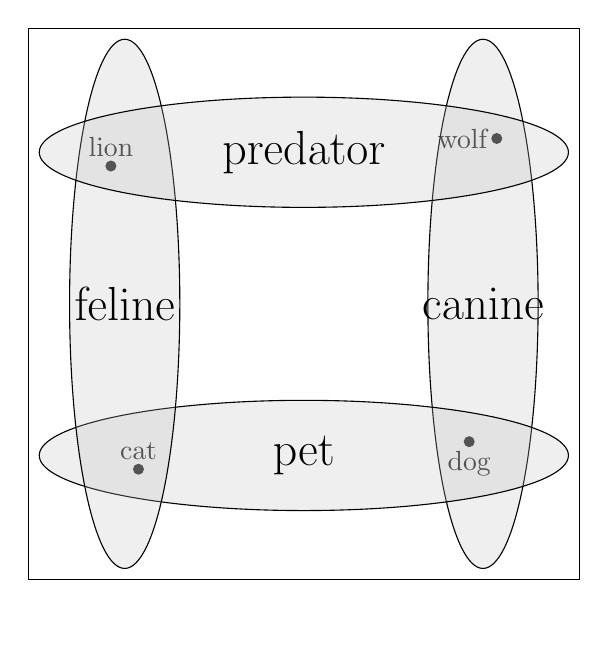
\begin{tikzpicture}[scale=0.07,baseline]
		\draw (0,0)--(-100,0)--(-100,-100)--(0,-100)--(0,0);
    	\draw (-15,-20) [left] node {wolf};
        \fill (-15,-20) circle[radius=1];
        \draw (-20,-75) [below] node {dog};
        \fill (-20,-75) circle[radius=1];
        \draw (-80,-80) [above] node {cat};
        \fill (-80,-80) circle[radius=1];
        \draw (-85,-25) [above] node {lion};
        \fill (-85,-25) circle[radius=1];
        \draw[fill=lightgray, fill opacity=0.25] (-17.5,-50) ellipse (10 and 48);
        \node at (-17.5,-50) {\LARGE canine};
        \draw[fill=lightgray, fill opacity=0.25] (-50,-77.5) ellipse (48 and 10);
        \node at (-50,-77.5) {\LARGE pet};
        \draw[fill=lightgray, fill opacity=0.25] (-82.5,-50) ellipse (10 and 48);
        \node at (-82.5,-50) {\LARGE feline};
        \draw[fill=lightgray, fill opacity=0.25] (-50,-22.5) ellipse (48 and 10);
        \node at (-50,-22.5) {\LARGE predator};
        \node at (-50,-102.5) [single arrow,draw,rotate=90,minimum height=40,minimum width=40,inner sep=15,opacity=0] {};
    \end{tikzpicture}
    \caption{a lexical space}
    \label{fig:bland}
    \end{subfigure}
    \begin{subfigure}[t]{0.5\textwidth}
    \centering
	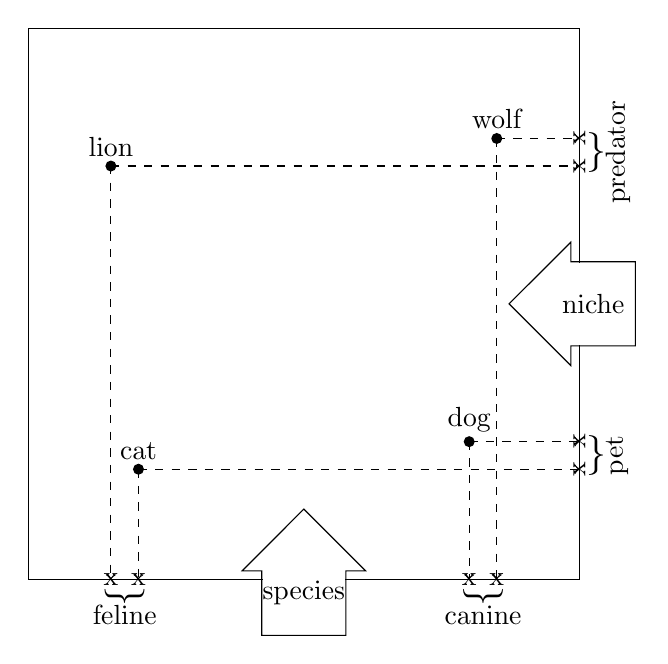
\begin{tikzpicture}[scale=0.07,baseline]
    	\draw (0,0)--(-100,0)--(-100,-100)--(-57.5,-100);
        \draw (-42.5,-100)--(0,-100)--(0,-57.5);
        \draw (0,-42.5)--(0,0);
    	\draw (-15,-20) [above] node {wolf};
        \fill (-15,-20) circle[radius=1];
        \draw[dashed,->] (-15,-20)--(-15,-100);
        \draw (-15,-100) node {x};
        \draw[dashed,->] (-15,-20)--(0,-20);
        \draw (0,-20) node [rotate=90] {x};
        
        \draw (-20,-75) [above] node {dog};
        \fill (-20,-75) circle[radius=1];
        \draw [dashed,->] (-20,-75)--(-20,-100);
        \draw (-20,-100) node {x};
        \draw [dashed,->] (-20,-75)--(0,-75);
        \draw (0,-75) node [rotate=90] {x};
        
        \draw (-80,-80) [above] node {cat};
        \fill (-80,-80) circle[radius=1];
        \draw [dashed,->] (-80,-80)--(-80,-100);
        \draw (-80,-100) node {x};
        \draw [dashed,->] (-80,-80)--(0,-80);
        \draw (0,-80) node [rotate=90] {x};
        
        \draw (-85,-25) [above] node {lion};
        \fill (-85,-25) circle[radius=1];
        \draw [dashed,->] (-85,-25)--(-85,-100);
        \draw (-85,-100) node {x};
        \draw [dashed,->] (-85,-25)--(0,-25);
        \draw (0,-25) node [rotate=90] {x};
        
        \node at (3,-22.5) [below,rotate=90] {predator};
        \node at (3,-22.5) {\Large\}};
		
        \node at (3,-77.5) [below,rotate=90] {pet};
        \node at (3,-77.5) {\Large\}};
		
        \node at (-17.5,-103) [below] {canine};
        \node at (-17.5,-103) [rotate=-90] {\Large\}};

        \node at (-82.5,-103) [below] {feline};
        \node at (-82.5,-103) [rotate=-90] {\Large\}};
        
        \node at (-50,-102.5) [single arrow,draw,rotate=90,minimum height=40,minimum width=40,inner sep=15] {};
        \node at (-50,-102.5) {species};
        \node at (2.5,-50) [single arrow,draw,rotate=180,,minimum height=40,minimum width=40,inner sep=15] {};
        \node at (2.5,-50) {niche};
    \end{tikzpicture}
    \caption{a contextual projection}
    \label{fig:perspective}
    \end{subfigure}
  \caption{In the two-dimensional space depicted in (a), the conceptual vagary of four words maps to overlapping, elongated and indeterminate spaces.  In (b), two different perspectives on the lexical space, represented by the arrows labelled \emph{niche} and \emph{species}, offer contextualised projections in one-dimensional clusters which remit conceptual clarity.}
\end{figure}

Furthermore, the high dimensionality of vector space models of distributional semantics in particular should afford precisely these types of contextual vistas on potential relationships between words.  Rather than depending on \emph{a priori} disambiguation based on clustering or observations of context in the form of existing combinations of words, I propose that a technique for defining subspaces \emph{in situ} will capture the momentary and situated way in which concepts come about in the course of a cognitive agent's entanglement with the world.  The way that relationships between words coalesce and then dissolve as we change our perspective on the space of this model is designed to reflect the way that concepts 

This description of a process of perspective taking has thus far been quite high-level: that high dimensional spaces afford different vantage points on data is evident, but this begs the question of the actual mechanism for defining perspectives in such spaces.  The next section will focus on answering this question by outlining a method for 

\section{Literal Dimensions of Co-Occurrence}
The model presented here is grounded within the paradigm of distributional semantics, which means that the conceptual geometries that it constructs are the product of observations of word co-occurrences in a large-scale corpus of textual data represented statistically.  Two procedurally distinct methodological regimens have emerged from the recent study of distributional semantics.  The first, and more established, approach involves tabulating word co-occurrence frequencies and then using some function over these to build up word-vector representations.  With roots in the frequentist analysis described by \cite{SaltonEA1975}, recent research has typically involved matrix factorisation techniques presented as either (or both) an optimisation technique \citep{BullinariaEA2012} or a noise reducing mechanism \citep{KielaEA2014}.\footnote{\cite{BullinariaEA2012}, \cite{LapesaEA2013}, and \cite{KielaEA2014} have all reported that dimensional reduction techniques including SVD, random indexing, and top frequency feature selection generally do not improve results on word similarity and composition tests, with some notable parameter specific exceptions.}  A more recent approach, which has received a great deal of attention with the increasing availability of large-scale data and the corresponding advent of complex neural network architectures, involves using non-linear regression techniques to iteratively learn word-vector representations in an online, stepwise traversal of a corpus \citep{BengioEA2003,CollobertEA2008,KalchbrennerEA2014}.  \cite{BaroniEA2014} have described the former as \emph{counting} and the latter as \emph{predicting}, but it must be noted that both methods are very much grounded in observations about the co-occurrence characteristics of vocabulary words across large bodies of text.

Another important similarity between these two approaches is that they each in their own way move towards a representation of relationships between word-vectors which is to some extent optimally informative, and, by the same token, abstract.  In the instance of neural network approaches, this is clearly the case due to the fundamental nature of the system: the dimensions of this variety of model exist as basically arbitrary handles for gradually adjusting the relative positions of vectors, slightly altering every dimension of each vector each time the corresponding word is observed in the corpus.  And, as far as models based on explicit co-occurrence counts are concerned, the favoured technique tends to involve starting with a large, sparse space of raw co-occurrence statistics (frequencies, or, more typically, a mutual information type metric) and then factorising this matrix using a linear algebraic technique such as singular value decomposition.  The result, in either case, is a space of vectors which exists just for the sake of placing words in a relationship where distance corresponds to a semantic property, consisting of dimensions which can only be interpreted in terms of the way that they allow the model to relate words, not in terms of their relationship to the underlying data.  In fact, \cite{LevyEA2014b} have argued that recently developed neural networks approaches just exactly do recapitulate the process of matrix factorisation, and that a careful tuning of hyperparameters will generate commensurable results from either type of model.

A key feature of the model proposed in this thesis is that it maintains a space of highly sparse co-occurrence statistics, which, despite their anchoring in the relatively abstract realm of word positions in a digitised corpus, I will describe as \emph{literal} in the sense that they can be interpreted as corresponding to actual relationships between words in the world.  I don't wish to claim that there is scope for completely or even mainly recapitulating a nuanced conceptual model from the data available in a purely textual environment; to do so would be to move towards claims that intentionality can emerge from rule-based operations on symbols, and the problems with this have been explored by \citepos{Searle1980} Chinese room argument and a subsequent generation of philosophers \citep{PrestonEA2002}.  But I would like to suggest that by building a base model that maintains the accessibility of unreduced co-occurrence information, we likewise maintain the ability to manipulate this base model extemporaneously, in reaction to the ongoing emergence of new contextual information.  The idea is that such a base model would essentially represent the superset of all possible dimensions available for \emph{ad hoc} selection in the course of a 

So the proper framework for describing the model to be examined in this thesis is not so much a single space of word-vectors as a Grassmannian lattice consisting of the power set of all possible combinations of the dimensions characterising the base space.  At the top of this lattice -- the \emph{join} -- sits a single $k$-dimensional space consisting of every available one of the $k$ co-occurrence terms observed throughout the underlying corpus.  At the bottom of the lattice -- the \emph{meet} -- sit $k$ different one-dimensional spaces, each space corresponding to a single co-occurrence term.  If the meet is considered $layer-1$ of the lattice, and the join is considered layer $k$, then any given interstitial $layer-j$ consists of every possible combination of $j$ dimensions of co-occurrence statistics.  A diagram of a very simple example of one such model is presented in Figure~\ref{fig:lattice}, illustrating the possible subspaces projected from a vastly simplified model consisting of just three co-occurrence dimensions (these particular spaces will be explored in the next section, as illustrated in Figure~\ref{fig:instruments}.

\begin{figure}
\centering
\begin{tikzpicture}[node distance=3cm,every node/.style={draw=black,thick,circle,inner sep=0pt}]
  \footnotesize
  \node[minimum size=2cm](join) {\begin{tabular}{c}
    \emph{cantata} \\
    \emph{sopranos} \\
    \emph{funk}
  \end{tabular}};
  \node[minimum size=2cm](two2) [below of=all] {\begin{tabular}{c}
    \emph{cantata} \\
    \emph{funk}
  \end{tabular}};
  \node[minimum size=2cm](two1) [left of=two2] {\begin{tabular}{c}
    \emph{cantata} \\
    \emph{sopranos}
  \end{tabular}};
    \node[minimum size=2cm](two3) [right of=two2] {\begin{tabular}{c}
    \emph{sopranos} \\
    \emph{funk}
  \end{tabular}};
  \node[minimum size=2cm](one2) [below of=two2] {\begin{tabular}{c}
    \emph{sopranos}
  \end{tabular}};
  \node[minimum size=2cm](one1) [left of=one2] {\begin{tabular}{c}
    \emph{cantata}
  \end{tabular}};
  \node[minimum size=2cm](one3) [right of=one2] {\begin{tabular}{c}
    \emph{funk}
  \end{tabular}};
  \draw (two1)--(join);
  \draw (two2)--(join);
  \draw (two3)--(join);
  \draw (one1)--(two1);
  \draw (one1)--(two2);
  \draw (one2)--(two1);
  \draw (one2)--(two3);
  \draw (one3)--(two2);
  \draw (one3)--(two3);
\end{tikzpicture}
\caption{A lattice of three dimensions, including the two-dimensional subspaces which are used for analysing the conceptual geometry of a small set of word-vectors in Figure~\ref{fig:instruments}}
\label{fig:lattice}
\end{figure}

An important distinction must be drawn, however, between the representation of my model as a lattice and the use of manifolds as an inferential mechanism.  Formal concept analysis in particular has made a productive discipline out of applying lattice type structures to conceptual modelling, using the semi-hierarchical properties of lattices to capture logical relationships of entailment \citep{Wille1982}.  That body of work takes as given that concepts are ``the basic units of thought formed in dynamic processes within social and cultural environments,'' \citep[][p. 2]{Wille2005}.  \cite{Widdows2004} offers a broad overview of how this approach might be pursued through corpus linguistic techniques, while \cite{GeffetEA2005} and, more recently, \cite{KartsaklisEA2016} have proposed statistical techniques using \emph{feature inclusion} metrics to assess the potential entailment relationship between candidate words and corresponding concepts.  The assumption inherent in this interesting work is that words are in some sense supervenient upon the concepts they denote, and that the statistical features of a language will by and large recapitulate the conceptual structure upon which it sits.

As \cite{Rimell2014} has pointed out, however, it is problematic to assume that a spectrum of co-occurrence alone can indicate relationships of hyponymy and hypernymy.  It stands to reason, for instance, that a word with a taxonomically specific referent such as \emph{bulldog} should probably have a co-occurrence profile including words omitted from the corresponding profile of a word like \emph{lifeform}, which has an ostensibly more general extent.  Rimell has proposed a measure of change in \emph{topic coherence} as word-vectors are combined algebraically in order to detect entailment relationships.  This measuring is achieved specifically through a process of dimension-by-dimensions comparison between potentially related word-vectors, in particular the \emph{vector negation} method described by \cite{Widdows2003}, combined with topic modelling techniques to analyse the coherence of features distilled by the selectional process.

The model proposed in this thesis adheres to the same principle of fine-grained cross-dimensional analysis described by Rimell.  In addition to the practical issues raised by Rimell, my model is also designed to remain pointedly uncommitted to any idea that concepts are atomic or elementary to thought, or that language and concepts are involved in any kind of strictly hierarchical relationships.  Instead, the model operates through an analytical traversal of a lattice of subspaces in search for a combination of dimensions that captures a conceptually \emph{salient} profile of co-occurrence features.  If a consequence of this stance is that the model can't be understood in terms of nested ordered relationships, though, then the question of how conceptual relationships do emerge situationally from the model remains.  The next section of this methodological overview will examine how the actual geometry of a projected subspace itself is expected to do this conceptual work.

\section{Interpretable Geometry}
It is important at this point to distinguish between two different modes of interpretability at play within the operation of the model I'm proposing.  On the one hand, we have the mechanism for selecting subspaces described above: this mechanism requires a model composed of tractable dimensions of statistics that can be interpreted based on expectations generated from an analysis of some sort of contextually relevant information.  Some specific mechanisms for this process will be discussed in the next section.  Then on the other hand, once this selectional process has taken place, we find ourselves with a subset of dimensions defining a specific subspace.  My claim is that, given the correct selectional criteria for performing this projection -- this traversal of our lattice of vector spaces -- we should be able to generate a subspace in which the projected word-vectors will be interpretable in terms of the actual geometric features of this subspace.

The idea of exploiting the geometry of a transformed space of word statistics is not new.  Indeed, seminal work on latent semantic analysis (LSA) was motivated by precisely the insight that a singular value decomposition of a high-dimensional, sparse matrix of statistical data about word co-occurrences would result in a dense lower dimensional matrix in which dimensions characterise \emph{latent semantics} rather than literal word co-occurrences \citep{DeerwesterEA1990}.  Thus the linear algebraic methodology of generating a lower dimensional matrix of optimally informative dimensions arguably transforms a space of specific co-occurrence events into a space of more general conceptual relationships.  In fact, \cite{LandauerEA1997} have subsequently argued that the dimensional reduction by way of factorisation itself might directly mirror cognitive conditioning, modelling the way that the mind can ``correctly infer indirect similarity relations only implicit in the temporal correlations of experience,'' (p. 212).

Of course the dimensions of a factorised matrix are still not interpretable in themselves.  They are, rather, an optimal abstraction of the underlying data, in which each dimension is maximally informative -- and, accordingly, orthogonal -- in comparison to the other dimensions.  What we desire in a model, however, is a mechanism for actually interpreting directions and regions within a subspace projected by the model.  This objective is motivated by \cite{Gardenfors2000} insight into the inferential power of \emph{conceptual spaces}: by building spaces in which the dimensions themselves correspond to \emph{properties}, G\"{a}rdenfors has illustrated how features of points and regions within these spaces such as convexity and betweeness can be interpreted as corresponding to conceptual membership and can accordingly be used to reason about relationships between concepts.  In more recent work, motivated by psycholinguist insight into the significance of the \emph{intersubjectivity} by which language facilitates the mutual ascription of cognitive content between interlocutors, \cite{Gardenfors2014} has proposed that semantics are derived from a communicative alignment of conceptual spaces.

A classic example of a G\"{a}rdenforsian conceptual space is the space of colors, which can be defined in terms of, for instance, hue, brightness, lightness, and colourfulness: any colour can be specified as a point corresponding to coordinates along each of these dimensions.  Moreover, regions within the space of colours can be defined geometrically: the concept \textsc{red} will correspond to a convex region within the space, and any point lying between two points known to be labelled \emph{red} will likewise be considered \emph{red}.  \cite{Jager} has devised an experiment mapping linguistic descriptions to conceptual regions precisely within the domain of colours.  Taking a large set of multi-lingual data regarding colour naming conventions, treating each of 330 different colours as an initially independent dimension, J\"{a}ger demonstrated how an extrapolation of optimally informational dimensions via a principle component analysis revealed clusterings of color names into convex regions.\footnote{The cross-cultural universality of colour naming conventions presented by \cite{KayEA1999}, which J\"{a}ger takes as a basis for his research, is controversial to say the least -- see \cite{Levinson2001} for an alternative point of view -- but J\"{a}ger's work remains a good example of a computational technique for extrapolating conceptual spaces from quantitative linguistic data.}

Similarly motivated by G\"{a}rdenfors's model of conceptual spaces, \cite{DerracEA2015} have built vectors of domain specific documents, associating word frequencies within documents with document labels.  A multi-dimensional scaling procedure is then used to project these document-vectors into a Euclidean space in which the authors predict that properties such as \emph{parallelness} and \emph{betweeness} will correspond to conceptual relationships between documents.  The authors demonstrate that geometry in their projected spaces does indeed afford conceptual interpretation: the word \emph{bog} is found to be more or less between \emph{heath} and \emph{wetland}, for instance, and the vector for the film \emph{Jurassic Park} lies in a direction associated with \textsc{dinosaurs} and \textsc{special effects}.  This work is particularly notable in that \citeauthor{DerracEA2015} appreciate the significance of projecting spaces which are interpretable in terms of Euclidean distances rather than simply the cosine similarity of vectors extending from the origin of a space: Euclidean metrics provide a platform for more nuanced considerations of the relationships between points.

The type of space exemplified by the research of J\"{a}ger and \citeauthor{Derrac} is moving towards being a conceptual space in the way that its geometry offers itself up to semantic interpretation, but importantly these remain static spaces comprised of abstract dimensions, albeit dimensions generated in order to optimise the interpretability of the spaces they delineate.  The objective of my model is to emulate the geometric interpretability of these other spaces in an extemporaneous, contextually dynamic way.  To illustrate this point, consider the two spaces illustrated in Figure~\ref{fig:instruments} (taken from real co-occurrence data, as described in the next section, and based on the lattice of subspaces illustrated in Figure~\ref{fig:lattice}).  Here co-occurrence statistics are used to define three different dimensions, from which two different two-dimensional subspaces are selected with word-vectors plotted into each subspace.  In each subspace, a particular conceptual geometry emerges, oblique to the axes of each subspace but nonetheless indicating distinct conceptual regions in which words cluster in an interpretable way.

\begin{figure}[t]
	\begin{subfigure}[t]{0.5\textwidth}
    \centering
	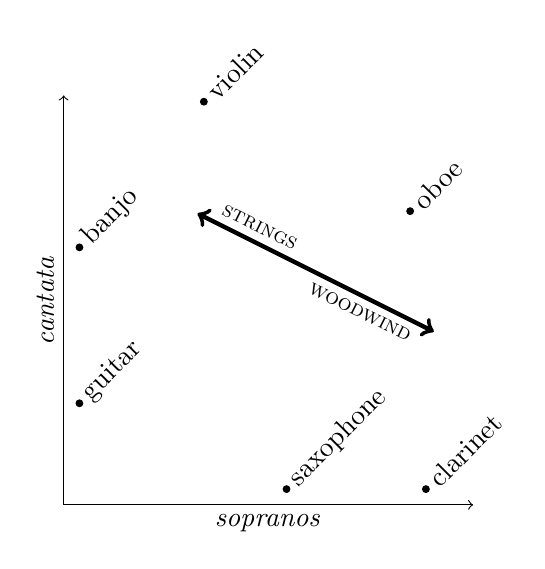
\begin{tikzpicture}[scale=1,baseline]
		\draw [->] (-0.2,-0.2)--(5,-0.2);
		\draw [->] (-0.2,-0.2)--(-0.2,5);
		\node at (2.4,-0.2) [below] {\emph{sopranos}};
		\node at (-0.2,2.4) [above,rotate=90] {\emph{cantata}};
		\draw [<->,ultra thick] (1.5,3.5)--(4.5,2);
		\node at (2.2,3.15) [above,rotate=-26.57] {\footnotesize \textsc{strings}};
		\node at (3.65,2.425) [below,rotate=-26.57] {\footnotesize \textsc{woodwind}};
		\node at (0.0,1.09) [right,rotate=45] {guitar};
		\fill (0.0,1.09) circle[radius=0.05];
		\node at (0.0,3.07) [right,rotate=45] {banjo};
		\fill (0.0,3.07) circle[radius=0.05];
		\node at (1.58,4.92) [right,rotate=45] {violin};
		\fill (1.58,4.92) circle[radius=0.05];
		\node at (2.63,0.0) [right,rotate=45] {saxophone};
		\fill (2.63,0.0) circle[radius=0.05];
		\node at (4.40,0.0) [right,rotate=45] {clarinet};
		\fill (4.40,0.0) circle[radius=0.05];
		\node at (4.20,3.53) [right,rotate=45] {oboe};
		\fill (4.20,3.53) circle[radius=0.05];
    \end{tikzpicture}
    \caption{\textsc{strings} vs \textsc{woodwind}}
    \label{fig:svsw}
    \end{subfigure}
    \begin{subfigure}[t]{0.5\textwidth}
    \centering
	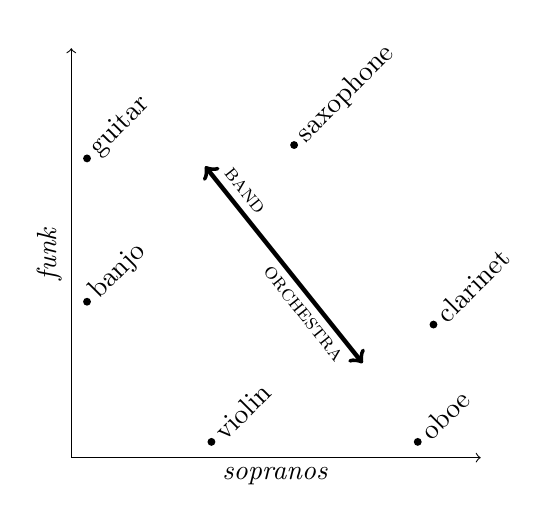
\begin{tikzpicture}[scale=1,baseline]
		\draw [->] (-0.2,-0.2)--(5,-0.2);
		\draw [->] (-0.2,-0.2)--(-0.2,5);
		\node at (2.4,-0.2) [below] {\emph{sopranos}};
		\node at (-0.2,2.4) [above,rotate=90] {\emph{funk}};
		\draw [<->,ultra thick] (1.5,3.5)--(3.5,1);
		\node at (1.85,3.0625) [above,rotate=-51.35] {\footnotesize \textsc{band}};
		\node at (2.9,1.75) [below,rotate=-51.35] {\footnotesize \textsc{orchestra}};
		\node at (0.0,3.60) [right,rotate=45] {guitar};
		\fill (0.0,3.60) circle[radius=0.05];
		\node at (0.0,1.78) [right,rotate=45] {banjo};
		\fill (0.0,1.78) circle[radius=0.05];
		\node at (1.58,0.0) [right,rotate=45] {violin};
		\fill (1.58,0.0) circle[radius=0.05];
		\node at (2.63,3.77) [right,rotate=45] {saxophone};
		\fill (2.63,3.77) circle[radius=0.05];
		\node at (4.40,1.49) [right,rotate=45] {clarinet};
		\fill (4.40,1.49) circle[radius=0.05];
		\node at (4.20,0.0) [right,rotate=45] {oboe};
		\fill (4.20,0.0) circle[radius=0.05];
    \end{tikzpicture}
    \caption{\textsc{band} vs \textsc{orchestra}}
    \label{fig:bvso}
    \end{subfigure}
  \caption{Based on real co-occurrence data, swapping one dimension in a two-dimensional subspace reveals two different conceptual geometries.}
  \label{fig:instruments}
\end{figure}

The first thing to note about these spaces is the way that swapping a single dimension in a two dimensional subspace can have a significant impact on the conceptual affordances of the subspace's geometry.  Realigning the relationships between terms along a single axis leads to a complete shift in the clusterings of terms, and, correspondingly, to the interpretation of regions and directions.  If these are conceptually sound subspaces, then we might expect word-vectors found within the area of the triangle described by the points labelled \emph{guitar}, \emph{banjo}, and \emph{violin} in Figure~\ref{fig:svsw} to be the names of other string instruments, or other conceptually relevant terms.  This is possibly asking too much of a subspace consisting of data regarding co-occurrences with just two terms across a large scale corpus, but as we scale up the dimensionality of the space -- as we ascend the lattice of subspaces of a fully realised model -- we can expect proper conceptual spaces to begin to coalesce.

The next thing to note is that the dimensions themselves are not especially interpretable.  While these dimensional profiles are explicable -- and indeed the ability to trace these statistics back to the corpus might turn out to be a desirable property for some applications -- the dimensions themselves do not conform to \citepos{Gardenfors2000} notion of dimensions as representing the properties that compose a concept.  It might be surprising, for instance, that the word \emph{cantata} has a higher propensity for co-occurrence with the word \emph{banjo} than with the word \emph{clarinet}, given that cantatas have traditionally included parts for the latter but not the former.  An examination of the underlying data, extracted, as described in the next section, from English language Wikipedia, reveals that the term \emph{cantata} has been adopted, perhaps somewhat figuratively, by some bluegrass musicians, and so co-occurrences with \emph{banjo} are indeed observed.

Rather than consider such usage as anomalous or attempt some sort of \emph{a priori} word sense disambiguation, I propose that we embrace the haphazardness of language and use it as a tool for projecting conceptually productive geometries.  In fact it would be surprising if it turned out that in anything other than the most specialised cases we could simply pick dimensions based on their labels and then expect co-occurrence statistics to play out in a conceptually coherent way, as this would contradict the Relevance Theoretic thesis that language in use is always significantly underspecified.  With this in mind, I suggest that we consider some set of dimensions, delineating a subspace and the corresponding geometry of word-vectors, to map precisely to a given context, and to effectively serve as the connective structure between language and conceptualisation.  Under this regimen, the dimensions themselves become the constitutive substance of a context, but they do not compositionally define any context in which they participate; rather, the contextualisation is an emergent property of the combination of dimensions underwriting it, corresponding to \emph{a way of speaking} about things.

The spaces illustrated in Figure~\ref{fig:instruments} are the product of a lattice consisting of combinations of just three dimensions, and as such the conceptual affordances of this toy model are highly limited.  As we add dimensionality to the model, however -- as we observe more terms co-occurring with our vocabulary of word-vectors -- we can expect an exponential growth in the combinatory possibilities of subspace construction.  With enough dimensions from which to choose, and with an appreciable degree of variance between the profiles of each dimensions, there should be scope for projecting more or less any constellation of word-vectors we desire.  The next question, then, is how to go about actually extracting a high dimensional base model of co-occurrence statistics from a large scale textual corpus.  The next section will answer this question.

\section{A Computational Process}
In this final section of this chapter, a technical implementation of the model described throughout the preceding three sections will be explained in detail.

\subsection{A Large Scale Textual Corpus}
The first step in a corpus based approach to natural language processing is the selection of the data which will provide the basis for our model.  I've picked the English language portion of Wikipedia as my data source, a choice which is in accordance with a good deal of work done in the field.  Some authors 

In the case of the model used throughout this thesis, the November 2014 dump of English language Wikipedia has been used.\footnote{Accessible at XXX}  A data cleaning process has been implemented, the first step of which is the chunking of the corpus into individual sentences.  Next parenthetical phrases are removed from each sentence, as these can potentially skew co-occurrence data, and all other punctuation is subsequently removed.  All characters are converted into lowercase to avoid words capitalised at the beginning of sentences, quotations, and other places from being considered as unique types.  Finally, the articles \emph{a}, \emph{an}, and \emph{the} are removed as they can distort co-occurrence windows (consider, for instance, how these terms affect the proximity of the other words in the phrase ``a mouse, an owl, and a dog sat on the moon'').  The cleaned corpus contains about

-WORD, SENTENCE COUNTS

As is generally the case with data cleaning, these measures are prone to error: for instance, due to the removal of punctuation, the contraction \emph{we're} will be considered identical to the word \emph{were}.  One of the strengths of the subspace projection technique that my model uses is its resilience to noise.  So, for instance, misspellings will be categorised as highly anomalous co-occurrence dimensions and are therefore unlikely to be contextually selected -- or, if they are regularly encountered enough to be contextually significant, there may well be useful information in the co-occurrence profile of such mistakes -- and essentially ubiquitous words are unlikely to provide context specific information, so the ambiguity between \emph{we're} and \emph{were} is unlikely to be drawn into any of the subspaces actually projected by the model.

From the cleaned corpus, the model's vocabulary is defined as the top 200,000 most frequently occurring word types.  This cut-off point is very close to the point where the total number of word tokens included -- that is, occurrences of any word of any type -- included by selecting all instances of all vocabulary words equals the total number of word types -- that is, unique word forms -- excluded.  Given the Zipfian distribution of word frequencies as observed throughout the corpus, this means that more than 95\% of the co-occurrence data available from the corpus will be taken into account by the model, while the number of word-vectors used to express this data represents less than 5\% of the potential vocabulary---a fairly efficient way of extrapolating statistics from the corpus.

- human vocabulary size

\subsection{Mutual Information of Word Co-Occurrences}
The critical event in the 

Here, following the example of almost all distributional semantic work, co-occurrence between a word $w$ and another word $c$ will be considered in terms of the number of other words between $w$ and $c$.  In the case of my model, again in accord with the a great deal of work within the field, a statistic for word $w$ in terms of its co-occurrence with $c$ will be derived from the consideration of all the times that $c$ is observed within $k$ words of $w$, where $k$ is one of the primary model parameters that will be considered in the experiments reported in later chapters of this thesis.  Based on these co-occurrence events, a matrix $M$ is defined, where rows consist of word-vectors, one for each of the 200,000 words in the vocabulary, and columns correspond to terms with which these vocabulary words co-occur.  These column-wise co-occurrence dimensions include the words in the vocabulary, including the possible co-occurrence of a word with itself (``a \emph{rose} is a \emph{rose} is a \emph{rose}'', for instance) as well as many, many words that are not in the vocabulary, to the extent that every word type in the corpus is considered as a dimension of co-occurrence.

In this last respect, my model diverges from the typical approach, which usually seeks to limit not only the vocabulary but also the dimensionality of the underlying co-occurrence matrix.  This has typically involved a curtailing of the number of co-occurrence terms at both ends of the frequency spectrum, based on the assumption that both high frequency so-called function words (the prepositions, conjunctions, and so forth) and low frequency terms such as obscure proper names will muddy a model with either general flattening or highly topical skewing.  In the case of my model, however, these problems are irrelevant, as dimensions will be selected on a case-by-case, context specific basis, and there is no good reason to discard information which may in some possibly unforeseen circumstance prove relevant.  The result is a 200,00 by \approx 7.5 million matrix $M$ where a scalar corresponding to co-occurrences between $w$ and $c$ is defined in terms of this equation:

\begin{equation}\label{eq:MI}
M_{w,c} = \log_2 \left(\frac{n_{w,c} \times W}{n_w \times \left(n_c + a\right)} + 1\right)
\end{equation}

Here $n_{w,c}$ represents the total number of times that that $c$ is observed as co-occurring in a sentence within $k$ words on either side of $w$, $n_w$ is the independent frequency of occurrences of $w$, and $c$ is likewise the overall frequency of $c$ being observed as a co-occurrence term throughout the corpus.  $W$ is the overall occurrence of all words throughout the corpus---and it should be noted that, excluding the term $a$, the ratio in Equation~\ref{eq:MI} is equivalent to the joint probability of $w$ and $c$ co-occurring.  The application of a logarithm to this ratio, again a common practice, is in the spirit of \citepos{Shannon} information theory, and is 

The term $a$ is a skewing constant used to prevent highly specific co-occurrences from dominating the analysis of a word's profile, set for the purposes of the work reported here at 10,000.\footnote{Anecdotally, the first combination of input words analysed during an early stage of the development of this model that didn't use a smoothing constant was the phrase ``musical creativity'', and the very first dimension indicated by the analysis was labelled \emph{gwiggins}---my primary supervisor's email handle.  Prof. Wiggins's deep connection with music and creativity meant that every instance of \emph{gwiggins} occurring throughout Wikipedia was in the vicinity of both \emph{musical} and \emph{creativity}, and so the dimension was indicated by the combination of these terms, which makes sense, but it was still a bit eerie to have such a personally relevant result generated by a model based on such general data.}

Finally, the entire ratio is skewed by 1 so that all values returned by the logarithm will be greater than 0, with a value of zero therefore indicating that two words have never been observed to co-occur with one another.  This is again a departure from standard practice, where, in word counting models, a \emph{pointwise mutual information} mechanism involving not skewing the ratio and instead treating any ratio of frequencies less than 1 -- that is, any co-occurrence that is observed less than often than balance of the mean values for all occurrences of $w$ and all co-occurrences with $c$ -- as being equivalent to 0, or no co-occurrence at all.  The motivation for this more typical technique is again to avoid incorporating unnecessary and potentially confounding information into a model, but, again, in the case of my model, the dimensional selection process will tend to ignore such information, and at the same time, as will be seen, data regarding relatively unlikely co-occurrences can sometimes also be quite informative.  In support of my technique, it is worth mentioning that the vast majority of potential co-occurrences will never be observed, and, at the same time, a comprehensive language model should maintain at least the possibility of any co-occurrence

\cite{Brown}

so there seems to be wisdom in the idea of not throwing away information about even relatively unlikely linguistic events.

\subsection{Dimensional Selection Techniques}
Having established a base model of co-occurrence statistics, the 

\begin{equation}\label{eq:oldNorm}
w^j_i = \frac{w^j_i}{\sqrt{\sum_{k=1}^{b} \left(w^k_i\right)^2}}
\end{equation}

\begin{equation}\label{eq:Norm}
w^j_i = \frac{w^j_i}{\sum_{k=1}^{b} abs\left(w^k_i\right)}
\end{equation}

\begin{equation}\label{eq:Arg}
\mu_c =  \frac{1}{n} \sum_{w=1}^{n}N_{w,c}
\end{equation}

\begin{equation}\label{eq:Trans}
M_{w,c} \Rightarrow S_{w,c'}
\end{equation}
\subsection{Extracting Semantics from Geometric Features}

%\chapter{Context Sensitive Distributional Semantics} \label{chap:method}
In the previous chapter, I laid down the theoretical groundwork for a distributional semantic methodology for dynamically establishing perspectives on statistical data about language use.  In this chapter, I'll describe the technical details for building a computational implementation of such a methodology.  The objective of this implementation is to establish a rigorous procedure for generating subspaces of word-vectors, based on observations of word co-occurrences in an underlying corpus, the geometries of which are semantically productive in particular contexts.  This will involve three steps:

\begin{enumerate}
\item The selection, processing, and analysis of a large scale textual corpus in order to create a high dimensional base space of co-occurrence statistics;
\item The development of techniques for selecting lower dimensional subspaces based on some sort of contextualising input;
\item The exploration of the geometry of the projected subspaces in search of semantic correlates.
\end{enumerate}

The following three sections will pursue each of these aspects of a technical implementation in turn.  The end result is effectively a mapping from text as raw data to geometry as semiotic generator.  A fourth section will describe an alternative, general interpretation of the statistical data which underwrites my models and additionally offer a brief overview of another distributional semantic methodology, both to be used as a point of comparison in the empirical results which will be discussed in subsequent chapters.

\section{Establishing and Analysing a Large Scale Corpus}
The first step in a corpus based approach to natural language processing is the selection of the data which will provide the basis for our model.  I've picked the English language portion of Wikipedia as my data source, a choice which is in accordance with a good deal of work done in the field.  For instance, \cite{GabrilovichEA2007} and \cite{CollobertEA2008}, to name just a couple, use Wikipedia as their base data for training distributional semantic models designed to perform tasks similar to the ones explored in subsequent chapters, while \cite{BaroniEA2014}, \cite{PenningtonEA2014}, and \cite{GutierrezEA2016} use amalgamated corpora that include Wikipedia as a major component.  Wikipedia provides a very large sample of highly regular language, meaning that we can expect a certain syntactic and semantic consistency as well as language which, if not always overtly literal, is likewise not typically abstruse or periphrastic.  This should supply a source of linguistic data in which, to revisit the central dogma of the distributional hypothesis, words which occur in a particular syntactic and lexical setting can be expected to be semantically similar.

In the case of my implementations, the November 2014 dump of English language Wikipedia has been used.\footnote{Relatively recent Wikipedia dumps are available at \url{https://dumps.wikimedia.org/}.}  A data cleaning process has been implemented, the first step of which is the chunking of the corpus into individual sentences.  Next parenthetical phrases are removed from each sentence, as these can potentially skew co-occurrence data, and all other punctuation other than hyphenation is subsequently removed.  All characters are converted into lowercase to avoid words capitalised at the beginning of sentences, quotations, and other places being considered as unique types.  Finally, the articles \emph{a}, \emph{an}, and \emph{the} are removed as they can distort co-occurrence distance counts, and then all sentences containing less than five words are discarded.  The cleaned corpus contains nearly 1.1 billion word tokens, consisting of almost 7.5 million unique word types spread across about 61 million sentences.  The distribution of these types is predictably Zipfian: over 10 million occurrences of each of the top nine word types are observed, while the least frequent 4.27 million words -- more than half of all types -- only occur once.  The top end of this distribution is populated by conjunctions, prepositions, and pronouns, while the bottom end is characterised by obscure place names, one-off abbreviations, unicode representing non-Latin alphabet spellings, and a good many spelling errors.

As is generally the case with data cleaning, these measures are prone to error: for instance, due to the removal of punctuation, the contraction \emph{we're} will be considered identical to the word \emph{were}.  One of the strengths of the subspace projection technique that my methodology uses is its resilience to noise.  So, for instance, misspellings will be categorised as highly anomalous co-occurrence dimensions and are therefore unlikely to be contextually selected -- or, if they are encountered regularly enough to be contextually significant, there may well be useful information in the co-occurrence profile of such mistakes -- while, at the other end of the spectrum, essentially ubiquitous words are unlikely to provide context specific information, so the ambiguity between \emph{we're} and \emph{were} is unlikely to be drawn into any of the subspaces actually projected by the model.

From the cleaned corpus, a model's vocabulary is defined as the top 200,000 most frequently occurring word types.  This cut-off point is very close to the point where the total number of word tokens included by selecting all instances of all vocabulary words equals the total number of word types excluded.  Given the Zipfian distribution of word frequencies as observed throughout the corpus, this means that more than 95\% of the co-occurrence data available from the corpus will be taken into account by the model, while the number of word-vectors used to express this data represents less than 5\% of the potential vocabulary---a fairly efficient way of extrapolating statistics from the corpus.  The selection of this as a cut-off point means that the least frequent words in the vocabulary occur 83 times throughout the corpus.

Having processed the corpus and established the target vocabulary, the next step of this methodology is to build up a base space of co-occurrence statistics.  Here, following the example of the majority distributional semantic work, co-occurrence between a word $w$ and another word $c$ will be considered in terms of the number of other words between $w$ and $c$.  In the case of my methodology, and again in accord with the a great deal of work within the field, a statistic for word $w$ in terms of its co-occurrence with $c$ will be derived from the consideration of all the times that $c$ is observed within $k$ words to either side of $w$ within the boundary of a sentence, where $k$ is one of the primary model parameters that will be considered in the experiments reported in later chapters of this thesis.  Based on these co-occurrence events, a matrix $M$ is defined, where rows consist of word-vectors, one for each of the 200,000 words in the vocabulary, and columns correspond to terms with which these vocabulary words co-occur.  These column-wise co-occurrence dimensions include the words in the vocabulary as well as many, many words that are not in the vocabulary, to the extent that every word type in the corpus is considered as a candidate for co-occurrence.  A \emph{pointwise mutual information} metric gauging the unexpectedness associated with the co-occurrence of two words is calculated in terms of this equation:

\begin{equation}\label{eq:MI}
M_{w,c} := \log_2 \left(\frac{f_{w,c} \times W}{f_w \times \left(f_c + a\right)} + 1\right)
\end{equation}

Here $f_{w,c}$ represents the total number of times that $c$ is observed as co-occurring in a sentence within $k$ words on either side of $w$, $f_w$ is the independent frequency of occurrences of $w$, and $f_c$ is likewise the overall frequency of $c$ being observed as a co-occurrence term throughout the corpus.  $W$ is the overall occurrence of all words throughout the corpus--and it should be noted that, excluding the term $a$, the ratio in Equation~\ref{eq:MI} is equivalent to the joint probability of $w$ and $c$ co-occurring.  The term $a$ is a skewing constant used to prevent highly specific co-occurrences from dominating the analysis of a word's profile, set for the purposes of the work reported here at 10,000.\footnote{Anecdotally, the first combination of input words analysed during an early stage of the development of this model that didn't use a smoothing constant was the phrase \emph{musical creativity}, and the very first dimension indicated by the analysis was labelled \emph{gwiggins}---the email handle of one of my supervisors.  Prof. Wiggins's deep connection with music and creativity meant that every instance of \emph{gwiggins} occurring throughout Wikipedia was in the vicinity of both \emph{musical} and \emph{creativity}, and so the dimension was indicated by its very high PMI value for each of these terms, which makes sense, but it was still a bit eerie to have such a personally relevant result generated by a model based on such general data.}  Finally, the entire ratio is skewed by 1 so that all values returned by the logarithm will be greater than 0, with a value of zero therefore indicating that two words have never been observed to co-occur with one another.

This last step of incrementing the ratio of frequencies in order to avoid values tending towards negative infinity in the case of very unlikely co-occurrences is again a departure from standard practice, where, in word counting models, a \emph{positive pointwise mutual information} mechanism involving not skewing the ratio and instead treating any ratio of frequencies less than 1 -- that is, any co-occurrence that occurs with a lower probability than the combined joint probability of independently observing $w$ and $c$ -- as being equivalent to zero \citep[][have considered a more general variable ratio shifting parameter]{LevyEA2014b}.  The motivation for this more typical technique is again to avoid incorporating unnecessary and potentially confounding information into a model, but, again, in the case of my model, the dimensional selection process will tend to ignore such information, and at the same time, as will be seen, data regarding relatively unlikely co-occurrences can sometimes also be quite informative.  Other variations on the distributional semantic approach include alternative treatments of the co-occurrence window, where some researchers have taken weighted samples or considered word order \citep{SocherEA2013b}, and also the processing of corpora, where part-of-speech and dependency tagging have been applied to positive effect \citep{PadoEA2007}.  \cite{LapesaEA2014} and \cite{MilajevsEA2016} offer comparative overviews of the effects of parameter variations on the performance of distributional semantic techniques.

The net result of my methodology is a matrix of weighted co-occurrence statistics, where higher values indicate a high number of observations of word $w$ co-occurring with word $c$ relative to the overall independent frequencies of $w$ and $c$.  Values of zero indicate words which have never been observed to co-occur in the corpus, and, as most words never co-occur with one another, the matrix is highly sparse.  The weighting scheme results in a kind of semi-normalisation of the matrix: infrequent words will tend to correspond to more sparse dimensions, but the non-zero values along these dimensions will for the same reason tend to be higher due to the lower value of the word's frequency in the denominator.  So far this technique sits comfortably within the scope of existing work in the field.  It is what I propose to do with this base matrix that will begin to distinguish my methodology, and this next step in the process of projecting context sensitive spaces of word-vectors will be discussed in the following section.

\section{Selecting Dimensions from a Sparse Co-Occurrence Matrix}
Context has thus far remained a somewhat abstract concept in this thesis.  In principle, the context in which conceptualisation occurs for a cognitive agent is its environment with all its affordances, linguistic and semantic but also more generally perceptual: in a word, the agent's \emph{umwelt} \citep{VonUexkull1957}.  In the world of physical entanglements, language presents itself with precisely the same open-ended opportunities for action as other modes of cognition \citep{Gibson1979,Clark1997}---and, in the case of language, the action afforded is meaning making.  In practice, however, context will be specified lexically, in terms of a word or set of words which are fed to a model, analysed in terms of their co-occurrence profiles, and then used to generate a subspace of conceptually relevant co-occurrence dimensions.  The intuition behind this approach is that there should be a set of dimensions which collectively represent a semantic tendency which can be mapped to a context, and this tendency should be discoverable in an analysis of the co-occurrence statistics of words which are exemplary of this way of talking about things.

%In practice, however, for the purposes of my methodology, context will be defined lexically, as a word or set of words which are fed to a model, analysed in terms of their co-occurrence profiles, and then used to generate a subspace of conceptually relevant co-occurrence dimensions.  The intuition behind this approach is the idea that there should be a set of words which collectively selects a set of dimensions that are conceptually relevant to some conceptual context, and the geometry of the word-vectors of my model vocabulary as projected into the subspace delineated by this set of dimensions should reveal the semantics of this context.

So, notwithstanding interesting work on multi-modal approaches to distributional semantics from, for instance, \cite{HillEA2014} and \cite{BruniEA2014}, with regard to the present technical description, I will treat \emph{contextual input} as meaning some set of words $T$ which have been selected for the purpose of performing some type of semantic evaluation and act as input to a context sensitive distributional semantic model.  The exact mechanisms for specifying $T$ will be discussed in subsequent chapters with regard to each of the individual experiments to be performed using my methodology; for now, I offer a general outline.  Each component of $T$ points to a word-vector in the matrix $M$ described in the previous section, and the collection of word-vectors corresponding to $T$ serve as the basis for an analysis leading to the projection of a context specific subspace $S$.  I propose three basic techniques for generating these projections, with the model parameter $d$ indicating the specified dimensionality of the subspace to be selected:

\begin{description}
\item[Joint] A subspace of $d$ dimensions with non-zero values for all elements of $T$ and the highest mean PMI values across all elements of $T$ is selected;
\item[Indy] The top $d/|T|$, where $|T|$ is the cardinality of $T$, dimensions are selected for each element of $T$ regardless of their values for other elements of $T$, and then these dimensions are combined to form a subspace with dimensionality $d$;
\item[Zipped] The top dimensions for each element of $T$ are selected as in the \textsc{indy} technique, with the caveat that all selected dimensions must have non-zero values for all elements of $T$ and no dimension is selected more than once.
\end{description}

These techniques are used for the purpose of analysis, and, once this analysis has been performed, the subset of dimensions returned is used to project the entire model vocabulary onto a $d$ dimensional subspace.  The \textsc{joint} technique requires the greatest finesse, as there is an element of cross-dimensional comparison at play.  As such, for the purposes of this technique, the word-vectors selected by $T$ are merged, dimensions with non-zero values for any of the word-vectors are discarded, and the resulting truncated word-vectors, each consisting of an equal number of non-zero dimensions, are normalised.  This ensures that certain elements of $T$ won't dominate the analysis: because the frequency of each word in $T$ applies a deflationary pressure on the PMI values associated with the corresponding word-vectors, very infrequent words would be liable to dominate the analysis with the associated high PMI values in their profile.  This effect is illustrated in Table~\ref{tab:norms}, where PMI values for the top dimensions selected using the \textsc{joint} type subspace by the words \emph{guitar}, which at 88,285 occurrences is ranked 1541 in frequency, are compared with those for the word \emph{dulcimer}, which occurs 516 times and is ranked 62,313 (the base model here was constructed using a 5x5 word co-occurrence window).  Among the dimensions with non-zero values for both words, normalisation brings the high end of the respective co-occurrence profiles more in line with one another, facilitating the selection of a subspace which is jointly characteristic of the input terms.

\begin{table}
\centering
\begin{tabular}{llrrlrrlrr}
\hline
& \multicolumn{3}{c}{\emph{guitar}} & \multicolumn{3}{c}{\emph{dulcimer}} \\
& dimension & PMI & normalised & dimension & PMI & normalised \\
\hline
\parbox[t]{2mm}{\multirow{5}{*}{\rotatebox[origin=c]{90}{\textsc{high}}}} & \emph{mandolin} & 8.30964 & 0.10719 & \multicolumn{1}{|l}{\emph{hammered}} & 13.97749 & 0.09354 \\
& \emph{bass} & 8.08501 & 0.10429 & \multicolumn{1}{|l}{\emph{dulcimer}} & 12.73992 & 0.08526 \\
& \emph{12-string} & 8.07679 & 0.10418 & \multicolumn{1}{|l}{\emph{autoharp}} & 11.50399 & 0.07699 \\
& \emph{acoustic} & 7.99076 & 0.10308 & \multicolumn{1}{|l}{\emph{appalachian}} & 11.23224 & 0.07517 \\
& \emph{banjo} & 7.96400 & 0.10057 & \multicolumn{1}{|l}{\emph{zither}} & 10.98302 & 0.07350 \\
\hline
\parbox[t]{2mm}{\multirow{5}{*}{\rotatebox[origin=c]{90}{\textsc{low}}}} & \emph{\emph{attacked}} & 0.05222 & 0.00067 & \multicolumn{1}{|l}{\emph{him}} & 0.25698 & 0.00172 \\
& \emph{report} & 0.04768 & 0.00062 & \multicolumn{1}{|l}{\emph{school}} & 0.25340 & 0.00170 \\
& \emph{country} & 0.04418 & 0.00057 & \multicolumn{1}{|l}{\emph{would}} & 0.23825 & 0.00159 \\
& \emph{champions} & 0.02644 & 0.00034 & \multicolumn{1}{|l}{\emph{into}} & 0.21336 & 0.00143 \\
& \emph{regions} & 0.02538 & 0.00033 & \multicolumn{1}{|l}{\emph{there}} & 0.21320 & 0.00143 \\
\hline
\end{tabular}
\caption[Highest and Lowest PMI Values]{The top five and bottom five dimensions by PMI value for the words \emph{guitar} and \emph{dulcimer}, out of all the dimensions with non-zero values for both words, with scores tabulated independently for each word.}
\label{tab:norms}
\end{table}

The intuition behind the construction of \textsc{joint} subspaces is that their dimensions should represent a profile of co-occurrences capturing the collective semantic characteristics of the contextual input.  By focussing on the terms that have strong co-occurrence tendencies for all of the word-vectors indicated by the input, the expectation is that these words will occupy a central region near the perimeter of the projected subspace, and other words in this region should be likewise conceptually associated with the input.  Expressed formulaically, a \textsc{Joint} subspace is delineated by a set $J$ of $d$ dimensions generated by the contextual input $T$ consisting of $k$ input terms mapping to word-vectors $\{t_1, t_2... t_k\}$.  These word-vectors are analysed to establish a $k \times j$ matrix $N$ consisting of $\{n_1, n_2... n_k\}$, the vectors of $T$ truncated such that they contain only the $j$ dimensions with non-zero values across $T$:

\begin{equation} \label{eq:subset}
%t_{h,i} \in m_h: \prod_{g=1}^{k} t_{g,i} > 0
n_h := \left \{t \in t_h: \prod_{g=1}^{k} t_{g,i} > 0\right \}
\end{equation}

\noindent $J$ is then composed by taking the $d$ dimensions with the highest mean values across a row-wise normalisation of $M$:

\begin{equation}
J := \left \{ f_{1...d} \in \argmax_{f}\left(\sum_{g=1}^{k} \frac{M_{g,f}}{||m_g||}\right)\right \}
\end{equation}-

\noindent In the cases of the \textsc{indy} and \textsc{zipped} techniques, the selectional process is more straightforward, since mean values between features of word-vectors are not being considered.  Where the \textsc{joint} technique is intended to discover subspaces that represent an amalgamation of the input terms, the \textsc{indy} technique is expected to produce a subspace where individual conceptual characteristics of the input terms, captured as collections of co-occurrence dimensions, are distilled into distinct geometric regions.  So the set of $d$ dimensions $I$ returned by the \textsc{indy} technique will delineate a subspace in which the relative geometry of contextual input word-vectors will reflect the degree to which the independent co-occurrence profiles of those word-vectors overlap.  So, given the set $B$ of all dimensions and the input word-vectors $\{t_1, t_2... t_k\}$, $I$ can be selected from this base set of dimensions:

\begin{equation}
I := \left \{b in B: t_{h,b} \geq \max_{d/k} t_h \right \}
\end{equation}

\noindent The \textsc{zipped} technique might be seen as something of a hybrid of the \textsc{joint} and \textsc{indy} techniques, since it used the \textsc{indy} approach to make selections from the intermediary space of non-zero dimensions available to the \textsc{joint} technique.  Here we know there will be some information about every co-occurrence dimensions for each word-vector associated with the contextual input, and so we might expect a subspace that offers a more nuanced interpretation of semantic relationships between the contextual input in particular.  The set of dimensions $Z$ delineating this space is selected from the same set $N$ described in Equation~\ref{eq:subset}, in this case simply selecting the dimensions with the highest values for each input word-vector, as they have non-zero values for all the input word-vectors:

\begin{equation}
Z := \left \{n \in N: t_{h,n} \geq \max_{d/k} t_h \right \}
\end{equation}

\noindent An import feature of the \textsc{indy} and \textsc{zipped} techniques is that in these subspaces, rare co-occurrence dimensions of the input terms are liable to have an impact on their geometric situation when these dimensions are selected by another input word-vector, so the preservation of all co-occurrence information in my methodology might be expected to prove valuable in these cases.  In each instance, these techniques are formulated to return a set of dimensions which, with varying degrees of cohesion, delineate a space that is in some sense salient to the contextual terms $T$ serving as the basis for the analysis.  In all cases, these techniques are used for the purpose of analysis, and, once this analysis has been performed, the subset of dimensions returned is used to project the entire model vocabulary onto a $d$ dimensional subspace.

In order to offer a sense of what's happening with these dimension selection techniques, a preliminary and intuitively motivated case study of dimension selection is outlined in Table~\ref{tab:dims}, again derived from a base space generated through observations made within a 5x5 word co-occurrence window over the course of the corpus.  The top dimensions selected by each technique are presented for two different three term sets of input words: \emph{lion}, \emph{tiger}, and \emph{bear}, on the one hand, which are taken to represent in their union exemplars of wild animals, and on the other hand \emph{dog}, \emph{hamster}, and \emph{goldfish}, which are prototypical pets.  The dimensions selected by the \textsc{joint} technique in response to the \textsc{wild animal} type input include the names of other wild animals, as well as \emph{paw}, a component of many wild animals, \emph{mauled}, an activity performed by wild animals, and, interestingly, \emph{mascot}, presumably because many sports teams take these types of animals as their mascot: while this connection may not be immediately intuitive, it seems likely that this word would probably select for other wild animals in terms of salient features of its co-occurrence profile.  The dimensions returned by the \textsc{indy} technique, on the other hand, are, as expected, more independently characteristic of each of the input terms, with culturally referential words like \emph{cowardly} (presumably from many mentions of the Cowardly Lion character from \emph{The Wizard of Oz}) and \emph{crouching} (indicating the context of the popular Chinese movie \emph{Crouching Tiger, Hidden Dragon}), as well as other species-specific terms such as \emph{sumatran} and \emph{grizzly}.  Notably, the term \emph{stearns} pops up here, certainly because of prolific references on Wikipedia to the defunct investment bank Bear Stearns, illustrating ways in which the \textsc{indy} technique might allow for dimensions indicative of underlying polysemy in some of their input terms.

\begin{table}
\centering
\begin{tabular}{llllll}
\hline
\multicolumn{3}{c}{\emph{lion, tiger, bear}} & \multicolumn{3}{c}{\emph{dog, hamster, goldfish}} \\
\textsc{joint} & \textsc{indy} & \textsc{zipped} & \textsc{joint} & \textsc{indy} & \textsc{zipped} \\
\hline
leopard & cowardly & cowardly & \multicolumn{1}{|l}{pet} & sled & dog \\
cub & crouching & sumatran & \multicolumn{1}{|l}{hamster} & hamster & hamster \\
hyena & localities & grizzly & \multicolumn{1}{|l}{goldfish} & goldfish & goldfish \\
sloth & rampant & tamer & \multicolumn{1}{|l}{hamsters} & hound & pet \\
lion & sumatran & leopard & \multicolumn{1}{|l}{domesticated} & djungarian & hamsters \\
mascot & grizzly & teddy & \multicolumn{1}{|l}{breed} & koi & fancy \\
paw & wardrobe & tamarin & \multicolumn{1}{|l}{fancy} & nassariidae & breed \\
tiger & leopard & tiger & \multicolumn{1}{|l}{pets} & ovary & siberian \\
rhinoceros & stearns & polar & \multicolumn{1}{|l}{bred} & carp & domesticated \\
mauled & teddy & passant & \multicolumn{1}{|l}{robotic} & ednas & cat \\
\hline
\end{tabular}
\caption[Top Dimensions for Wild Animals]{The top 10 dimensions returned using three different dimensional selection techniques, featuring one set of input terms collectively referring to wild animals and another set collectively referring to pets.}
\label{tab:dims}
\end{table}

Similar effects are observed in response to the \textsc{pet} type input.  The word \emph{pet}, two of the three input terms themselves, and the names of other types of pets appear in the output from the \textsc{joint} technique, as well as descriptive terms such as \emph{domesticated}, \emph{breed}, and, amusingly but not irrelevantly, \emph{robotic}, presumably because of the phenomenon of robotic pets, which has its own page on Wikipedia.  The \textsc{indy} technique, on the other hand, returns some very term specific dimensions, again indicating a degree of ambiguity, such as \emph{djungarian} (a breed of hamster popular as a house pet), \emph{nassariidae} (in fact a species of snail, known colloquial as the \emph{dog whelk}), and \emph{ednas} (Edna's Goldfish was a short-lived but often cited American punk rock band).  In the cases of both \textsc{pets} and \textsc{wild animals}, the dimensions returned by the \textsc{zipped} technique represent something of an intermediary between the two other techniques, tending to include some of the terms generated using the \textsc{joint} technique but also some more word-specific terms.  The actual geometry of these spaces will be discussed generally in the next section, and will be explored in detail in relation to specific semantic applications in subsequent chapters.

A very broadly similar approach to distributional semantics has been proposed by \cite{PolajnarEA2014}, who describe a \emph{context selection} methodology for generating word-vectors, involving building a base space of co-occurrence statistics and then transforming this space by preserving only the highest values for each word-vector up to some parametrically determined cut-off point, setting all other values to zero.  Setting the cut-off point relatively stringently -- generating a base space of more sparse word-vectors, followed by various dimension reduction techniques -- led to improvements in results on both word similarity and compositionality tests.  This suggests that allowing word-vectors to shed some of their more obscure co-occurrence statistics leads to a more sharply defined semantic space, and indeed there may be an element of disambiguation at play here, as well, with vectors dropping some of the features associated with less frequent alternate word senses.

In the end, though, the method described by \citeauthor{PolajnarEA2014} results in a space which, while the information contained in the representation of a particular word is to a certain extent focused on the most typical co-occurrence features of that word, is still fundamentally general and static.  To the extent that any contextualisation takes place here, it happens \emph{a priori} and is cemented into a fixed spatial relationship between word-vectors.  This is anathema to the theoretical grounding of my methodology, which holds that conceptual relationships arise situationally, and that semantic representations should therefore likewise come about in an \emph{ad hoc} way.  The novelty, and, I will argue, the power of my approach lies in its capacity to generate bespoke subspaces in reaction to semantic input as it emerges, and the expectation is that these subspaces will have a likewise context specific geometry which can be explored in order to discover situationally significant relationships between the projected semantic representations.  The next section will begin to examine how these geometries might look.

\section{Exploring the Geometry of a Context Specific Subspace}
Before delving into the question of the types of geometries my method might be expected to generate, I would like to raise a point regarding the typical application of the term \emph{geometry} to vector space models of distributional semantics in the first place.  \cite{Widdows2004} makes an enthusiastic and compelling case for the representational power of geometry, while \citeauthor{Clark2015} has pointed out that treating words as geometric features endows lexical representations with ``significant internal structure'' \citep[][p. 509]{Clark2015} which can be applied towards modelling the meaning making compositionality of language.  \cite{BaroniEA2014b} go so far as to suggest that their distributional semantic model effectively instantiates the abstract principles of Frege's work on the logic of natural languages \citep{Dummett1981} in a geometric mode.  These are powerful points touching on the essence of semiotics, and the idea that representations that map from data to interpretable features in a space are core to my own methodology, as discussed in Chapter~\ref{chap:lexsem}.

The point I would like to make now, though, is that there are different degrees of geometry that can be in principle accessed in a vector space of real valued dimensions.  The great majority of approaches surveyed here, taken to be representative of the historical and ongoing trend in the field, present models consisting of spaces of normalised word-vectors, in which there is a monotonic correlation between the distance and the angle between two word-vectors.  In the case of models built using a principal component analysis, this is because when the eigenvectors of a matrix factorisation are used as dimensions of maximal variance, there is no meaningful interpretation of the actual values along these dimensions; in fact, mean values along a dimension will tend towards zero and the signs of values along any dimension discovered through a singular value decomposition can be reversed without any degradation of the information available from analysis \citep{AbdiEA2010}.  So, while Euclidean distance is strictly meaningful in such a dimensional reduction, there is no sense of a centre of the space other than the centre of gravity of the data as projected onto the selected number of eigenvectors, and cosine similarity is in practice the measure used to determine the similarity between two word-vectors.  And in the case of models built using neural networks, there is no meaningful interpretation of dimensions to begin with, so the resulting space is a \emph{de facto} hypersphere of word vectors that are only relative in terms of their relationship to one another, not their relationship to any objective features of the space.

In the case of my methodology, however, precise values along dimensions, and, correspondingly, overall Euclidean distances are significant: because base dimensions are preserved in the spaces projected through any of the dimension selection techniques described above, the actual position of word-vectors in space, not just their relative situations on the surface of a normal hypersphere, are significant, with a number of potentially desirable effects.  The first effect to note is that in my subspaces distance from the origin is expected to be a meaningful feature.  In a subspace of contextually selected dimensions, word-vectors with strong co-occurrence tendencies for that set of dimensions should have high PMI values across all dimensions, and so a relatively high norm of a word-vector is anticipated to correspond to semantic saliency within that context.

The second effect is that there is a notion of centre and periphery in my subspaces.  Since all values are positive, a word-vector with high scores across all or most dimensions in a subspace will be far from the origin and in the central region of the space.  A further consequence of the positivity of these subspaces is that word-vectors with mainly low or null PMI values will be far from the centre, so in the end two word-vectors may be both close to the centre of a subspace, or at the periphery of a subspace but close to one another, or at the periphery and far from each other, at two different edges of the positively valued space, and each of these situations can be predicted to have a particular semantic interpretation.  The third effect, which follows from the first two points, is that a subspace can be characterised in terms of a set of key points based on an analysis of the collective profiles of the dimensions delineating the subspace, by which I mean some straightforward assessments of the statistical distribution of each dimension involved.  This aspect of my subspaces will be examined in more detail in Chapter~\ref{chap:replete}; first, though, I'll consider a couple basic measures for analysing word-vectors in context.

\begin{figure}%[!ht]
  \centering%\vspace*{-2cm}
  \begin{subfigure}[]{0.45\textwidth}
  \centering
  \small
  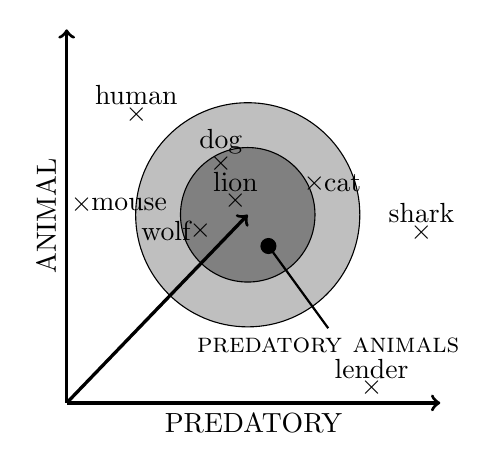
\begin{tikzpicture}
%    \begin{axis}[disabledatascaling,scale=1.75,axis equal,hide axis]
    \begin{axis}[disabledatascaling,scale=1,axis equal,hide axis]
%      \draw [fill = lightgray,fill opacity = 1.00] (3,3) circle [radius = 1.5];
%      \draw [fill = gray,fill opacity = 1.00] (3,3) circle [radius = 0.9];
      \draw [fill = lightgray,fill opacity = 1.00] (2.423,2.518) circle [radius = 1.5];
      \draw [fill = gray,fill opacity = 1.00] (2.423,2.518) circle [radius = 0.9];
      \node at (4.7477,2.2786) [above] {shark};
      \node at (4.7477,2.2786) {$\times$};
      \node at (2.0626,3.2008) [above] {dog};
      \node at (2.0626,3.2008) {$\times$};
      \node at (3.3145,2.9414) [right] {cat};
      \node at (3.3145,2.9414) {$\times$};
      \node at (4.0803,0.2) [above] {lender};
      \node at (4.0803,0.2) {$\times$};
      \node at (2.258,2.7022) [above] {lion};
      \node at (2.258,2.7022) {$\times$};
%      \draw [dotted] (3,3)--(2.258,2.7022) node [midway,above] {$a$};
      \node at (1.7883,2.3021) [left] {wolf};
      \node at (1.7883,2.3021) {$\times$};
      \node at (0.9311,3.8643) [above] {human};
      \node at (0.9311,3.8643) {$\times$};
%      \draw [dotted] (3,3)--(0.9311,3.8643) node [midway,above] {$b$};
      \node at (0.2,2.6516) [right] {mouse};
      \node at (0.2,2.6516) {$\times$};
      
      \addplot [->,very thick] coordinates{
      	(0,0)
        (2.423,2.518)
      };
      \node at (3.5,1.0) [below] {\textsc{predatory animals}};
      \addplot [thick] coordinates{
        (3.5,1.0)
        (2.7,2.1)
      };
      \draw [fill=black] (2.7,2.1) circle [radius = 0.1];
%      \addplot [->,dashed] coordinates{
%        (3,3)
%        (3.7,2.4343)
%      } node [midway,below] {$r_1$};
%      \addplot [->,dashed] coordinates{
%        (3,3)
%        (2.1,4.2)
%      } node [midway,above] {$r_2$};
      \addplot [->,very thick] coordinates{
        (0,0)
        (0,5)
      } node [midway,above,sloped] {ANIMAL};
      \addplot [->,very thick] coordinates{
        (0,0)
        (5,0)
      } node [midway,below] {PREDATORY};
    \end{axis}
  \end{tikzpicture}
  \caption{Word-vectors measured by proximity to a central point.}\label{fig:geo1-dist}
  \end{subfigure}
  \hspace*{0.05\textwidth}
  \begin{subfigure}[]{0.45\textwidth}
  \centering
  \small
  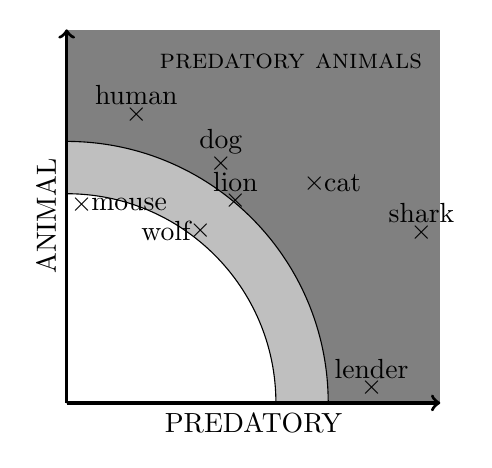
\begin{tikzpicture}
    \begin{axis}[disabledatascaling,scale=1,axis equal,hide axis]
      \draw [white,fill = gray,fill opacity = 1.00] (0,0) rectangle (5,5);
      \draw [fill = lightgray,fill opacity = 1.00] (0,0) -- (3.5,0) arc (0:90:3.5);
      \draw [fill = white,fill opacity = 1.00] (0,0) -- (2.8,0) arc (0:90:2.8);
      \node at (4.7477,2.2786) [above] {shark};
      \node at (4.7477,2.2786) {$\times$};
      \node at (2.0626,3.2008) [above] {dog};
      \node at (2.0626,3.2008) {$\times$};
      \node at (3.3145,2.9414) [right] {cat};
      \node at (3.3145,2.9414) {$\times$};
      \node at (4.0803,0.2) [above] {lender};
      \node at (4.0803,0.2) {$\times$};
      \node at (2.258,2.7022) [above] {lion};
      \node at (2.258,2.7022) {$\times$};
%      \draw [dotted] (0,0)--(2.258,2.7022) node [midway,above] {$a$};
      \node at (1.7883,2.3021) [left] {wolf};
      \node at (1.7883,2.3021) {$\times$};
      \node at (0.9311,3.8643) [above] {human};
      \node at (0.9311,3.8643) {$\times$};
%      \draw [dotted] (0,0)--(0.9311,3.8643) node [midway,above] {$b$};
      \node at (0.2,2.6516) [right] {mouse};
      \node at (0.2,2.6516) {$\times$};
      
      \node at (3,4.8) [below] {\textsc{predatory animals}};
%      \addplot [->,dashed] coordinates{
%        (0,0)
%        (2.8723,2.0)
%      } node [midway,below] {$r_1$};
%      \addplot [->,dashed] coordinates{
%        (0,0)
%        (2.6153,1.0)
%      } node [midway,above] {$r_2$};
      \addplot [->,very thick] coordinates{
        (0,0)
        (0,5)
      } node [midway,above,sloped] {ANIMAL};
      \addplot [->,very thick] coordinates{
        (0,0)
        (5,0)
      } node [midway,below] {PREDATORY};
    \end{axis}
  \end{tikzpicture}
  \caption{Word-vectors meansured in terms of distance from origin.}\label{fig:geo1-norm}
  \end{subfigure}
  \caption[Two Methods for Probing a Subspace]{Co-occurrence statistics for a small vocabulary construed along two hand-picked dimensions.  Darker regions are expected to be more conceptually prototypical for the context captured by these dimensions.}\label{fig:geo1}
\end{figure}

\subsection{Two Measures for Probing a Subspace} \label{sec:twomeasures}

In order to take a first pass at examining these robustly Euclidean features of my contextualised subspaces, I propose two geometric measures for exploring the conceptual geometry of a subspace, illustrated in Figure~\ref{fig:geo1}.  The first is a distance metric, which defines a central point in a subspace and then considers the relationship of words to the semantic context of the subspace in terms of the distance of the corresponding word-vectors from this central point.  The central point is defined as the mean point between the input word-vectors used to generate the subspace, or, for the purposes of Figure~\ref{fig:geo1-dist}, the central point of the eight word-vectors being analysed in this context.  In this subspace featuring two hand picked co-occurrence dimensions selected from a base model built from a 5x5 word co-occurrence window traversal of Wikipedia, word-vectors relatively closely associated with the concept \textsc{predatory animal} turn up near this central point.\footnote{Here it happens to be the case that choosing dimensions which actually nominate a concept likewise delineate a space where, at least in terms of the restricted vocabulary evoked in Figure~\ref{fig:geo1}, conceptual membership plays out in a geometrically predictable way, but I will not generally presume this to be the case.}  So, for instance, cats (certainly in their taxonomical sense), more specifically lions, dogs, and, again more specifically, wolves all fall close to the central point, while sharks (certainly predators, and also animals, but perhaps less prototypically so), mice, humans, and lenders are more distant.

The second measure deployed here will be to analyse the norms of the word-vectors projected into the contextualised subspace, with my hypothesis being that word-vectors that are relatively far from the origin will be correspondingly relevant to the conceptual context from which the subspace has been generated.  This prediction does not entirely play out in the subspace depicted in Figure~\ref{fig:geo1-norm}, where words like \emph{human} and \emph{lender} are about as far from the origin as \emph{cat} and \emph{shark}, and have higher norms than more prototypical denotations such as \emph{lion} and \emph{wolf}.  As will be seen in subsequent results, beginning here and extending into the experiments described in the next chapter, in higher dimensional subspaces selected using the techniques outlined above, norm does prove to be a predictive measure of semantic relevance.  Here again, the preponderance of co-occurrence statistics associated with a word over the course of a set of dimensions gives a higher dimensional subspace an advantage: if the selected dimensions are appropriately aligned, there will be a tendency for those word-vectors with some consistency of co-occurrence across all dimensions to extend towards the central fringe of the space, while those with inconsistent co-occurrence profiles will move towards the edges while remaining closer to the origin.

In the cases of both the distance from mean and norm measures, a threshold could, in principle, be established in order to determine a cut-off point for conceptual membership, either in terms of an absolute geometric measure -- a radius from either the central point or the origin -- or in terms of a set of nearest neighbours.  This move would begin to move these subspaces towards \citepos{Gardenfors2000} notion of a region within a conceptual space, particularly in the case of the distance based metric illustrated in Figure~\ref{fig:geo1-dist}: here a clear sense of convexity as a criterion for a conceptual region exists, and likewise of betweeness as an indicator of conceptual inclusion.  Importantly, though, these spaces as they stand lack the dimensional interpretability that characterises G\"{a}rdenfors's spaces, in that it is not possible to say that there is a dimension of size, or strength, or ferocity, or so forth along which a boundary for inclusion in the concept of \textsc{predatory animal} can be identified.

%\begin{table}
%\centering
%\small
%\begin{tabular}{ll|ll|ll|ll}
%\hline
%\multicolumn{4}{c}{\emph{lion, tiger, bear}} & \multicolumn{4}{|c}{\emph{dog, hamster, goldfish}} \\
%\multicolumn{2}{c}{\textsc{joint}} & \multicolumn{2}{c}{\textsc{indy}} & \multicolumn{2}{|c}{\textsc{joint}} & \multicolumn{2}{c}{\textsc{indy}} \\
%\hline
%norm & distance & norm & distance & norm & distance & norm & distance \\
%\hline
%leopard & cat & leopard & wild & hamsters & cat & dogs & cat \\
%langur & wild & dhole & cat & gerbils & pet & hamsters & giant \\
%hyena & wolf & hyena & giant & rabbits & monkey & sheepdog & animal \\
%dhole & elephant & rhinoceros & elephant & chinchillas & pig & terrier & wild \\
%boar & animals & leopards & lions & pet & rabbit & canine & animals \\
%tapir & giant & tapir & wolf & ferrets & rat & kennel & like \\
%macaque & animal & passant & animals & pigs & animal & akc & rabbit \\
%chital & bears & langur & tigers & rats & dogs & spaniel & include \\
%civet & dog & sumatran & cats & pets & giant & poodle & pig \\
%sloth & panther & gules & golden & chickens & cats & jerboa & cats \\
%\hline
%\end{tabular}
%\caption{The top word-vectors in spaces selected by input terms characteristic of \textsc{wild animals} and \textsc{pets}, for the \textsc{joint} and \textsc{indy} dimension selection techniques, measured in terms of top norms within each subspace and also word-vectors closest to the mean point between the input word-vectors.}
%\label{tab:tops}
%\end{table}

\begin{table} \label{tab:wild}
\centering
\begin{tabular}{lll|lll}
\hline
\multicolumn{6}{c}{\emph{lion, tiger, bear}} \\
\multicolumn{3}{c}{\textsc{joint}} & \multicolumn{3}{c}{\textsc{indy}} \\
\hline
norm & distance & angle & norm & distance & angel \\
\hline
leopard & cat & and & leopard & wild & and \\
langur & wild & like & dhole & cat & as \\
hyena & wolf & also & hyena & giant & which \\
dhole & elephant & as & rhinoceros & elephant & like \\
boar & animals & such & leopards & lions & also \\
tapir & giant & well & tapir & wolf & be \\
macaque & animal & including & passant & animals & more \\
chital & bears & include & langur & tigers & including \\
civet & dog & from & sumatran & cats & been \\
sloth & panther & which & gules & golden & one \\
\hline
\end{tabular}
\caption[Top Wild Animal Word-Vectors]{The top word-vectors in subspaces selected by input terms characteristic of \textsc{wild animals}, for the \textsc{joint} and \textsc{indy} dimension selection techniques, measured in terms of top norms within each subspace (\emph{norm}), word-vectors closest to the mean point between the input word-vectors (\emph{distance}), and also the smallest angle with this mean vector regardless of actual position in the subspace (\emph{angle}).}
\label{tab:tops-wild}
\end{table}

Examples of the tendencies of both norms and relative distances are explored in Table~\ref{tab:tops-wild} and Table~\ref{tab:tops-pet}, where, as with the examples offered earlier in this chapter, input terms denoting things exemplary of the respective concepts \textsc{wild animals} and \textsc{pets} are used to generate subspaces, in this case using both the \textsc{joint} and \textsc{indy} dimension selection techniques, once again using a base space built using a 5x5 word co-occurrence window.  In these cases, the top 200 dimensions derived using each technique have been used to project subspaces, and then within those subspaces, the top ten word-vectors based on their norm and their distance from the mean point between the input word-vectors are reported.  In addition to the two geometric measures described above, as a point of comparison, I also present results using an angular measure, where the word-vectors with the highest cosine similarity with the vector of the mean point between the input word-vectors are returned.  This is offered as an approximation of what would be a typical approach in a standard static distributional model, to demonstrate why this measure doesn't work for the context sensitive spaces built using my methodology and also as a mechanism for further exploration of what's happening in these subspaces.

\begin{table} \label{tab:pet}
\centering
\begin{tabular}{lll|lll}
\hline
\multicolumn{6}{c}{\emph{dog, hamster, goldfish}} \\
\multicolumn{3}{c}{\textsc{joint}} & \multicolumn{3}{c}{\textsc{indy}} \\
\hline
norm & distance & angle & norm & distance & angle \\
\hline
hamsters & cat & and & dogs & cat & also \\
gerbils & pet & also & hamsters & giant & as \\
rabbits & monkey & as & sheepdog & animal & in \\
chinchillas & pig & of & terrier & wild & which \\
pet & rabbit & in & canine & animals & and \\
ferrets & rat & such & kennel & like & like \\
pigs & animal & well & akc & rabbit & is \\
rats & dogs & - & spaniel & include & called \\
pets & giant & called & poodle & pig & of \\
chickens & cats & which & jerboa & cats & has \\
\hline
\end{tabular}
\caption[Top Pet Word-Vectors]{The top word-vectors in subspace, as in Table~\ref{tab:tops-wild} but selected by input terms characteristic of \textsc{pets}.}
\label{tab:tops-pet}
\end{table}

Notably, in the case of the norm measure, word-vectors that are exemplary of the conceptual category suggested by the intersection of the input terms seem to rise to the top of the subspace, so to speak: for both dimension selection techniques for the \textsc{wild animal} type inputs, a list of wild animals, some rather exotic, are returned.  A similar outcome is observed for the norm measure in the case of the \text{pet} inputs, with some admittedly disputable admissions such as \emph{rats} coming up in the \textsc{joint} output; jerboas, which are indicated in the \textsc{indy} output, are apparently a somewhat popular pet, and \emph{akc} presumably refers to the American Kennel Club, so, not a pet, but an institution related to pet keeping.  An interesting side effect of the \textsc{indy} technique in particular is that it returns a list including names of various dog breeds.  It would seem that the co-occurrence dimensions of the word-vectors for \emph{hamster} and \emph{goldfish} are characteristic enough of these more specialised words relating to particular types of pets that the corresponding word-vectors are pushed towards the outer fringe of the subspace.  It's also interesting that \emph{passant} and \emph{gules}, terms associated with the depiction of animals in heraldry, have high norms in the \textsc{indy} subspace for \textsc{wild animal} input in particular---of course all three of the input terms here are denotations of animals typical of heraldic devices, so it is not particularly surprising that some of their independently strong co-occurrence features combine to select for these word-vectors.

The distance measure returns roughly similar results, including a number of denotations of appropriate animals.  Here it is interesting to observe that other semantic types -- in particular, adjectives in addition to nouns -- begin to creep into the output: \emph{wild}, \emph{giant}, and \emph{golden} are returned in the \textsc{joint} and \textsc{indy} subspaces for the \textsc{wild animal} input, and \emph{giat} again comes up in response to the \textsc{pets} input, along with, perplexingly, the verb \emph{include}.  It makes sense that the region near the mean point between the input vectors, where consistently high but perhaps not absolutely maximal PMI scores across these contextually characteristic dimensions are to be found, feature some of the descriptors and predicates associated with the concept being modelled, while the region at the outer fringe of the space, where the words with the highest overall PMI values across the dimensions of the subspace, would be pointed denotations of instances of the concepts in question.  The word-vectors corresponding to some of the more esoteric animals in particular are likely to have high co-occurrence frequencies with the same dimensions selected by the combination of the input terms relative to low independent frequencies precisely because of their rareness.

Turning to the angular results, where words that are closest to the line extending through the mean point are returned, a sharp contrast to the other two geometric measures is observed.  Here, very generic words which serve as the structural components of language, contributing little in terms of specific meaning but crucial to the functional cohesion of an utterance, are found in abundance.  This is completely logical: these types of words are liable to have a very consistent, albeit relatively low, profile of PMI scores across all dimensions in a subspace, since they are likely to have a high frequency of co-occurrences with any given word mitigated by a correspondingly high independent frequency across the corpus influencing the denominator of the PMI calculation.  The result is a word-vector populated by relatively low but also relatively consistent PMI values, situated not far from the origin and also very close to the centre line of the subspace.  This phenomenon highlights the discrepancy between the Euclidean, positively valued subspaces generated by my context sensitive methodology and the normalised, hyperspherical spaces built by conventional static distributional semantic models.  Because my subspaces have a sense of centre and periphery, as well as a sense of distance from the origin, it is possible to make both semantic and functional predictions about the types of words that will be found in different regions of a subspace, and accordingly to predict where to look -- and where not to look -- to discover geometries mapping to desired conceptual properties.

\subsection{Replete Geometric Analysis} \label{chap:replete}
I will now propose a general method for a replete geometric analysis of a contextually projected subspace, based on the position of word-vectors in a space as well as the relationship between those word-vectors and points based on a more general analysis of the dimensions delineating the subspace which I will characterise as \emph{generic points}.  For the purposes of explicating this method, I will presume a subspace projected from an analysis of two input word-vectors $A$ and $B$ using one of the dimension selection techniques described earlier in this chapter, a presumption in line with the experiments to be described in Chapters~\ref{chap:literal} and~\ref{chap:figurative}.  The premise is that these word vectors are to be analysed in terms of their semantic relationship; the precise nature of the relationship being analysed could be more or less anything, and in the next two chapters this method will be applied to the assessment of lexical similarity, relatedness, metaphor, and metonymy.  The objective of this analytic method will be first to test the hypothesis that the geometry of contextually projected subspaces should be semantically informative, and second to compare the aspects of the geometry that are most informative for different semantic phenomena.

\begin{figure}
\centering
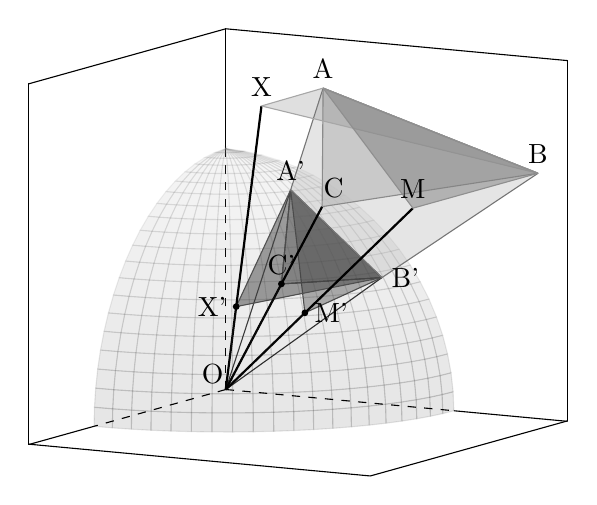
\begin{tikzpicture}
\begin{axis}[axis line style=white,view={120}{10},xmin=0,xmax=1.5,ymin=0,ymax=1.5,zmin=0,zmax=1.5,colormap/blackwhite,ticks=none]
\addplot3[color=black,thick] coordinates {(0,0,1.5) (0,1.5,1.5)};
\addplot3[color=black,thick] coordinates {(0,0,1.5) (1.5,0,1.5)};
\addplot3[color=black,thick] coordinates {(0,1.5,0) (0,1.5,1.5)};
\addplot3[color=black,thick] coordinates {(0,1.5,0) (1.5,1.5,0)};
\addplot3[color=black,thick] coordinates {(1.5,0,0) (1.5,0,1.5)};
\addplot3[color=black,thick] coordinates {(1.5,0,0) (1.5,1.5,0)};
\addplot3[color=black,dashed] coordinates {(0,0,0) (0,0,1)};
\addplot3[color=black,dashed] coordinates {(0,0,0) (0,1,0)};
\addplot3[color=black,dashed] coordinates {(0,0,0) (1,0,0)};
\addplot3[color=black] coordinates {(0,0,1) (0,0,1.5)};
\addplot3[color=black] coordinates {(0,1,0) (0,1.5,0)};
\addplot3[color=black] coordinates {(1,0,0) (1.5,0,0)};
\addplot3[patch,patch type=triangle,color=gray,fill opacity=0.0] coordinates {(0.0,0.0,0.0) (0.5774,0.5774,0.5774) (0.2,0.4,0.8944)
};
\addplot3[patch,patch type=triangle,color=gray,fill opacity=0.0] coordinates {(0.0,0.0,0.0) (0.5774,0.5774,0.5774) (0.2,0.8,0.5657)
};
\addplot3[patch,patch type=triangle,color=darkgray,fill opacity=0.25] coordinates {(0.5774,0.5774,0.5774) (0.2,0.4,0.8944) (0.2,0.8,0.5657)
};
\addplot3[patch,patch type=triangle,color=darkgray,fill opacity=0.4] coordinates {(0.5709,0.6766,0.4651) (0.2,0.4,0.8944) (0.2,0.8,0.5657)
};
\addplot3[patch,patch type=triangle,color=darkgray,fill opacity=0.5] coordinates {(0.7309,0.4678,0.4970) (0.2,0.4,0.8944) (0.2,0.8,0.5657)
};
\addplot3 [color=black,thick] coordinates {(0,0,0) (0.5774,0.5774,0.5774)};
\addplot3 [color=black,thick] coordinates {(0,0,0) (0.7309,0.4678,0.4970)};
\addplot3 [color=black,thick] coordinates {(0,0,0) (0.5709,0.6766,0.4651)};
\addplot3[opacity = 0.1,surf,z buffer = sort,samples = 21,variable = \u,variable y = \v,domain = 0:90,y domain = 0:90,]
    ({1*cos(u)*sin(v)}, {1*sin(u)*sin(v)}, {1*cos(v)});
\addplot3 [patch,patch type=rectangle,color=lightgray,fill opacity=0.4] coordinates{(0.2,0.4,0.8944) (0.3,0.6,1.35) (0.4,1.6,1.1) (0.2,0.8,0.5657)};
\addplot3 [color=black,thick] coordinates {(0.5774,0.5774,0.5774) (1.0,1.0,1.0)};
\addplot3 [color=black,thick] coordinates {(0.7309,0.4678,0.4970) (2.5,1.6,1.7)};
\addplot3 [color=black,thick] coordinates {(0.5709,0.6766,0.4651) (1.35,1.6,1.1)};
\addplot3 [patch,patch type=triangle,color=lightgray,fill opacity=0.75] coordinates{(0.3,0.6,1.35) (1.0,1.0,1.0) (0.4,1.6,1.1)};
\addplot3 [patch,patch type=triangle,color=gray,fill opacity=0.25] coordinates{(0.3,0.6,1.35) (2.5,1.6,1.7) (0.4,1.6,1.1)};
\addplot3 [patch,patch type=triangle,color=gray,fill opacity=0.5] coordinates{(0.3,0.6,1.35) (1.35,1.6,1.1) (0.4,1.6,1.1)};
\node [anchor=south] at (axis cs: 0.1,0.0,0.0) {O};
\node [anchor=south] at (axis cs: 0.3,0.6,1.35) {A};
\node [anchor=south] at (axis cs: 0.4,1.6,1.1) {B};
\node [anchor=south] at (axis cs: 0.2,0.4,0.8944) {A'};
\node [anchor=west] at (axis cs: 0.2,0.8,0.5657) {B'};
\node [anchor=south] at (axis cs: 0.5774,0.5774,0.5774) {C'};
\draw plot [mark=*, mark size=1] coordinates{(axis cs: 0.5774,0.5774,0.5774)};
\node [anchor=south] at (axis cs: 1.0,1.05,1.0) {C};
\node [anchor=east] at (axis cs: 0.7309,0.4678,0.4970) {X'};
\draw plot [mark=*, mark size=1] coordinates{(axis cs: 0.7309,0.4678,0.4970)};
\node [anchor=south] at (axis cs: 2.5,1.6,1.7) {X};
\node [anchor=west] at (axis cs: 0.5709,0.6766,0.4651) {M'};
\draw plot [mark=*, mark size=1] coordinates{(axis cs: 0.5709,0.6766,0.4651)};
\node [anchor=south] at (axis cs: 1.35,1.6,1.1) {M};
\end{axis}
\end{tikzpicture}
\caption[Geometric Features of Contextualised Subspaces]{The geometric features of a subspace contextually projected based on an analysis of two input word-vectors.}
\label{fig:geofull}
\end{figure}

Figure~\ref{fig:geofull} illustrates a generic three dimensional subspace, with point $O$ as the origin.  Points $A$ and $B$ are the two word-vectors that have been used to select the dimensions which define this subspace, and are likewise the word-vectors which will be analysed through the geometry of the subspace.  In addition to these two points explicitly defined in terms of the values of projected word-vectors, two points are established based on an overall analysis of the dimensionality of the subspace: the \emph{mean point} $M$ and the \emph{maximal point} $X$.  $M$ is defined as the vector of all the mean values for all the dimensions $J$ delineating the subspace, so, if the dimensionality of $J$ is $d$, M can be defined formally as follows:

\begin{equation}
M := \{\mu(J_{1}),\ \mu(J_{2})...\ \mu(J_{d})\}
\end{equation}

\noindent And likewise, $X$ can be expressed in terms of an equation:

\begin{equation}
X := \{max(J_{1}),\ max(J_{2})...\ max(J_{d})\}
\end{equation}

\noindent Finally, a generic central point $C$, a vector with all dimensions set to the same value, is defined.  The universal value chosen to define the dimensions of this vector is the mean value of the mean point $M$, so, formally, this point is the vector of that mean value repeated $d$ times:

\begin{equation}
C := \{\mu(M),\ \mu(M)... \mu(M)\}
\end{equation}

\noindent In the analysis of the semantic relationship between $A$ and $B$ in a given projection, these three vectors will be used as anchor points to establish the situation of $A$ and $B$ relative to the subspace overall: where $C$ is an objectively central point in the subspace, $M$ is in a sense central to a subspace relative to its particular dimensional constitution, and $X$ is similarly indicative of the outermost possible extent of a particular subspace.  The underlying intuition here is that, due to the frequentist components of the information theoretic co-occurrence statistics used to build the base space, different dimensions have different distributional profiles.  To demonstrate this point, Table~\ref{tab:profiles} presents the mean values and standard deviations for the distribution of mean and maximum points from the top 20,000\footnote{less frequent dimensions tend to have higher PMI values overall, and also tend to be products of co-occurrences observed in quite obscure passages of the base corpus---it's worth recalling that a little more than half of the co-occurrence dimensions are observed only once.} most frequent co-occurrence dimensions, as well as the top five and bottom five values for each of these statistics for illustrative purposes.

\begin{table}
\centering
\begin{tabular}{lr|r}
\hline
& \multicolumn{1}{c}{\textsc{mean}} & \multicolumn{1}{c}{\textsc{max}} \\
\hline
\parbox[t]{2mm}{\multirow{5}{*}{\rotatebox[origin=c]{90}{\textsc{top}}}} & \emph{sofla:} 6.984 & \emph{nico:} 15.690 \\
& \emph{olya:} 6.326 & \emph{yeah:} 15.610 \\
& \emph{non-families:} 6.035 & \emph{superfamily:} 15.598 \\
& \emph{gmina:} 5.364 & \emph{eel:} 15.483 \\
& \emph{crambidae:} 5.485 & \emph{kermanshah:} 15.455 \\
\hline
\parbox[t]{2mm}{\multirow{5}{*}{\rotatebox[origin=c]{90}{\textsc{bottom}}}} & \emph{it:} 0.748 & \emph{he:} 3.903 \\
& \emph{they:} 0.812 & \emph{in:} 3.449 \\
& \emph{you:} 0.804 & \emph{of:} 3.379 \\
& \emph{this:} 0.789 & \emph{to:} 3.120 \\
& \emph{he:} 0.719 & \emph{and:} 2.993 \\
\hline
mean & 2.312 & 11.066 \\
std & 0.396 & 1.607 \\
\hline
\end{tabular}
\caption[Mean and Maximum PMI Values]{Dimensional profiles in terms of mean and maximum PMI values along dimensions, including mean values and standard deviation as well as the top five and bottom five dimensions for each statistic.}
\label{tab:profiles}
\end{table}

The co-occurrence dimensions that tend to have lower mean and maximum values are clearly quite frequent words, and this is to be expected, given that the high frequency of independent observations of the word will drive PMI scores down for that word across the board.  The emergence of relatively infrequent words at the top end of the spectrum is then also to be expected.\footnote{The appearance of \emph{yeah} as one of the dimensions with a particular high maximum value is interesting, and perhaps surprising, though it should be noted that this is a particularly un-Wikipedian word, and is likely to occur in the context of things like quotations and band names, where co-occurrence with likewise obscure terms is more likely.}  The main point to note here, though, is that there is a broad range of possible mean and maximum values for a given dimension, and so the points $M$ and $X$ might be expected to vary considerably from subspace to subspace.  Moreover, this variance may in turn correspond to semantic features of a given subspace: it may be the case that a given type of relationship between input terms -- terms which are similar or dissimilar, literal or figurative in relationship to one another -- select for a subspace which has a particular orientation in terms of its dimensional profile.  A final observation here regards the way that the distribution of mean and maximum dimensional values skew, with means tending to clump towards the low end of the spectrum while maximums are more dense at the high end of the spectrum.  More specific conjectures and results will be presented throughout the next two chapters.

In addition to the situation of the points $A$, $B$, $C$, $M$, and $X$ in a subspace, a normalised version of the subspace is considered, in which each vector is effectively measured at its intersection with a hypersphere of radius 1 emanating from the origin.  These points are represented as $A'$, $B'$, $C'$, $M'$, and $X'$ respectively in Figure~\ref{fig:geofull}.  The purpose of considering these points is to take measure of the way in which the various vectors in a given subspace relate to the subspace as a whole, regardless of the extent of these vectors.  So, for instance, the vectors $A$ and $B$ might have very different norms, but the distances $A'$, $B'$, $C'$, $M'$, and $X'$ might still be very small---and, even then, the angle $\angle A'M'B'$ might be very large, suggesting that $A$ and $B$ both pass through the central region of the subspace but on different sides of the generic central point of the subspace.  One of the objectives of this analytical method is to test whether this kind of information, which can be captured through a robust geometric description of a subspace, is semantically indicative.

So finally the various geometric features available for the analysis of a subspace are systematically outlined in Table~\ref{tab:features}.  The points to be found in the space are broken down into three types, namely, the word-vectors themselves (points $A$ and $B$), the generic points that emerge from an analysis of a subspace (points $C$, $M$, and $X$), and the normalised versions of all these points ($A'$, $B'$, $C'$ $M'$, and $X'$).  The relationships between these points are construed across five categories as follows:

\begin{description}
\item[Distances] Euclidean distances, such as the distance between the two word-vectors $A$ and $B$ as well as the norms of the generic points, and, additionally, the mean distance of $A$ and $B$ from the origin;
\item[Angles] The angles at the vertexes of the generic points of a subspace, so for instance $\angle ACB$ formed by lines $\overline{AC}$ and $\overline{BC}$, as well as the normalised versions of these angles, and also the angles formed between the vectors of the generic points such as $\angle COM$;
\item[Means] The average norms of the word-vectors and the average distances from the word-vectors to generic points as well as the average distances of the normalised versions of these points;
\item[Ratios] The ratio of the norms of the word-vectors and of the distances from the word-vectors to generic points, taking the lower of the two distances as the denominator, as well as the normalised version of the same measures;
\item [Fractions] The ratio of the mean distance from the origin of $A$ and $B$ to each of the three generic points, as well as the ratios of the generic points to one another.
\end{description}

\begin{table}
\centering
\begin{tabular}{ll}
\hline
\multicolumn{2}{c}{\textsc{distances}} \\
word-vectors & $\overline{AB}$ \\
generic points & $C$, \quad $M$, \quad $X$ \\
\hline
\multicolumn{2}{c}{\textsc{angles}} \\
word-vectors & $\angle AOB$, \quad $\angle ACB$, \quad $\angle AMB$, \quad $\angle AXB$ \\
normalised & $\angle A'C'B'$, \quad $\angle A'M'B'$, \quad $\angle A'X'B'$ \\
generic points & $\angle COM$, \quad $\angle COX$, \quad $\angle MOX$ \\
\hline
\multicolumn{2}{c}{\textsc{means}} \\
word-vectors & $\mu (A,B)$, \quad $\mu (\overline{AC},\overline{BC})$, \quad $\mu (\overline{AM},\overline{BM})$, \quad $\mu (\overline{AX},\overline{BX})$ \\
normalised & $\mu (\overline{A'C'},\overline{B'C'})$, \quad $\mu (\overline{A'M'},\overline{B'M'})$, \quad $\mu (\overline{A'X'},\overline{B'X'})$ \\
\hline
\multicolumn{2}{c}{\textsc{ratios}} \\
word-vectors & $A:B$, \quad $\overline{AC}:\overline{BC}$, \quad $\overline{AM}:\overline{BM}$, \quad $\overline{AX}:\overline{BX}$ \\
normalised & $\overline{A'C'}:\overline{B'C'}$, \quad $\overline{A'M'}:\overline{B'M'}$, \quad $\overline{A'X'}:\overline{B'X'}$ \\
\hline
\multicolumn{2}{c}{\textsc{fractions}} \\
word-vectors & $\mu (A,B)/C$, \quad $\mu (A,B)/M$, \quad $\mu (A,B)/X$ \\
generic points & $C/M$, \quad $C/X$, \quad $M/X$ \\
\hline
\end{tabular}
\caption[Schematic of Geometric Features]{Geometric features extrapolated from a subspace projected based on an analysis of two two input terms $A$ and $B$.}
\label{tab:features}
\end{table}

\noindent These features have been selected as indicative of the overall comportment of the subspaces from which they are extracted, and, both independently and in conjunction, are expected to serve as indicators of the semantic phenomena characteristic of the word-vectors used to generate the subspace into which they are projected.  So, for instance, I will predict (incorrectly, it turns out) that the distance $\overline{AB}$ will be one of the strongest indicators of semantic relatedness.  Furthermore, the extrapolation of the generic features of a subspace is expected to indicate more general patterns of co-occurrence that are associated with semantic phenomena such as similarity and metaphor.  When dimensions with similar mean value are jointly selected by a pair of words, a (more correct) expectation will be that this indicates a high degree of conceptual overlap between the words' referents, and therefore a high degree of similarity.

As a more general hypothesis, I surmise that different sets of geometric features will collectively be predictive of different semantic phenomena.  One of the primary objectives of the empirical work described in the next two chapters will be to establish a methodology for mapping features to phenomena and then using these correspondences as a mechanism for understanding the statistical characteristics that allow for the computational extraction of semantically and contextually useful information from large scale corpora.  It will therefore ultimately be the comparison of the groupings of features corresponding to specific semantic phenomena that will provide the most significant outputs of the research reported here, and so the arrangement of features in terms of types and categories as outlined in Table~\ref{tab:features} is in this regard a schematic for the computational experimentation and corresponding evaluation and analysis at the core of this thesis.

\section{A Mathematical Justification for Geometric Analysis} \label{sec:math}
The application of geometry as a productive analytical tool for extrapolating semantic information from contextualised co-occurrence statistics has been, thus far, presented as a somewhat intuitive decision.  There is a certain elegance to using quantifiable distances and angles as the analytical representation of choice, and this approach will, it will be seen, assist in the visualisation of what's happening statistically in the subspaces produced by my model.  Notwithstanding these benefits, this section will offer a more mathematically thorough explanation of why a geometric approach is the right one for the types of statistics that are being used here, and in probabilistic models in general.

In order to understand the usefulness of geometry, it is worthwhile to consider again the information theoretical nature of the statistics being used here, and more generally in a plethora of distributional semantic models.  Specifically, revisiting and restating Equation~\ref{eq:MI}, the scalars of the base model are defined by considering a ratio of frequencies approximately equivalent to a ratio of probabilities:

\begin{equation}
PMI(w,c) \approx \log\left(\frac{p(w,c)}{p(w) \times p(c)}\right)
\end{equation}

\noindent In other words, PMI values are logarithms of probabilities, and logarithms have the natural property of translating products and ratios into sums and differences.  So, for instance, if we have an operation such as $PMI(w_1,c)-PMI(w_2,c)$, we can express this as a log of a ratio of products of probabilities:

\begin{equation}
PMI(w_1,c)-PMI(w_2,c) \approx \log\left(\frac{p(w_1,c) \times p(w_2) \times p(c)}{p(w_2,c) \times p(w_1) \times p(c)} \right)
\end{equation}

\noindent This, in turn, actually just reduces to a ratio of conditional probabilities:

\begin{equation} \label{eq:logdif}
PMI(w_1,c)-PMI(w_2,c) \approx \log\left(\frac{p(c|w_1)}{p(c|w_2)}\right)
\end{equation}

\noindent Next it must be noted that the geometry of the features described in Table~\ref{tab:features} are in large part derived from the vectors between the various points of interest -- word-vectors as well as generic features -- in a contextualised subspace.  These vectors can now be understood as concatenations of logarithms of ratios of the pointwise conditional probabilities of the dimensions delineating a $d$ dimensional context:

\begin{equation}
\overrightarrow{w_1}-\overrightarrow{w_2} \approx \left\{ \log\left(\frac{p(c_1|w_1)}{p(c_1|w_2}\right), \log\left(\frac{p(c_2|w_1)}{p(c_2|w_2)}\right)... \log\left(\frac{p(c_d|w_1)}{p(c_d|w_2)}\right)\right\}
\end{equation}

\noindent So from this perspective, the various features used to analyse the semantic situation of lexical representations in a contextualised subspace are, in fact, operations on conditional probabilities derived from observations of co-occurrence dimensions in the vicinity of target words.  This then becomes a recapitulation of my hypothesis, namely, that there should be a mechanism for exploring how the semantic context in which word meaning comes about can be captured in terms of a way of talking about things, with this way of talking mapping more specifically to a set of conditional probabilities relating to the chances of finding a particular context term in the vicinity of a target word (or, indeed, the average or maximal probability of finding that context term, as with the non word-vector features of a subspace).  Then the dimensional selection techniques proposed earlier in this chapter are now effectively three postulates about methods for discovering the set of co-occurrence terms which should be considered in the context of the conditions of target word-vectors and generic points in a subspace.

Furthermore, when we consider the various geometric features of a contextualised subspace as the independent variables of a model designed to classify or quantify a semantic phenomenon, we are in fact looking for weighted linear combinations of operations on conditional probabilities that maximise the correlation between those statistics and a set of dependent variables generally based on human observations.  In Chapter~\ref{chap:literal}, for instance, a linear regression will be used to try to learn to predict human ratings of relatedness and similarity based on geometric features of subspaces, and in Chapter~\ref{chap:figurative} a logistic regression will be used to similarly classify binary judgements of metaphoricity.  At this point, the geometry of the subspaces generated by my methodology becomes not only a convenient mechanism for humans to use to visualise the relationships between various statistical spaces, but actually also a handle for an algorithm to selectively learn rather complex combinations of probabilistic features.  A machine learning approach to analysing the geometry of a contextualised subspace then becomes a mechanism for iterating through inferential expressions formulated as operations on conditional probabilities, and an effective model will extrapolate an interpretable treatment of these probabilities directly from the geometry of a subspace.

This more or less sets the stage for the empirical section of the thesis.  The only outstanding issue is the establishment of the models which will serve as consistent points of comparison for my methodology.

\section{Comparing to Alternative Approaches}
In order to evaluate the effectiveness of my methodology, it will naturally be necessary to compare the performance of the models I develop against other models.  One way of doing this will, of course, be to compare to results other researchers have obtained experimenting with the data which will serve as the foundation for the results reported in the next two chapters.  In the cases of results reported by other researchers, though, similar but variously different corpora have been used to train other models described in the literature.  This is to be expected, and the results for large scale corpora should be fairly generalisable assuming a sensible choice of data (and the use of Wikipedia as all or a large portion of base data is quite common in the field), but nonetheless it will be useful to establish a baseline of results generated using models trained on the exact corpus to which I apply my methodology.  And in the cases of metaphor and semantic type coercion in particular, which will be examined in Chapter~\ref{chap:figurative}, the datasets explored are relatively new and have not been approached by many researchers in the field, so any additional point of comparison will be valuable in evaluating my methodology.

Moreover, in most cases, other models have been designed in a task specific way: so, for instance, \cite{SchwartzEA2015} have developed a syntactic heuristic for identifying semantic similarity as compared to relatedness in particular, and \cite{GutierrezEA2016} describe a model that generates compositional adjective-noun representations geared towards metaphor detection.  One of the key features of my models is that they are intended to be \emph{general}: the geometries generated by my methodology are expected to be replete with semantic interpretability, allowing for the same potential for diverse and often surprising conceptualisation corresponding to the infinitely combinatory characteristic of natural language in use.  For this reason, it is desirable to have a base case of a generic model that can be compared across the board to all the different tasks handled by my methodology.

With all this in mind, I propose two different points of comparison that, in addition to results extracted from existing literature, will be applicable to all subsequent experiments described here.  The first involves factorising my base space using singular value decomposition (SVD), abstracting the space into a smaller set of abstract dimensions representing axes of maximum variance between PMI values.  The second is an application of a well known and highly productive neural network model to the same underlying data that I've used.  This will serve as a mechanism for comparing my results to what has proved to be another very effective methodology for the statistical modelling of semantics in general.

\subsection{Static Interpretations of the Base Space}
Using the dimension reduction techniques described by, for instance, \cite{DeerwesterEA1990} in the context of latent semantic analysis, it is possible to directly transform the same base spaces used for my context sensitive projections into a static model consisting of word-vectors defined along dimensions abstracted away from co-occurrence statistics in order to instead represent maximal axes of variance across the underlying data.  The mathematical technique applied here is a low rank approximation of a singular value decomposition of the full blown co-occurrence matrix.  To revisit this linear algebraic procedure, a $c \times d$ co-occurrence matrix $M$ can be decomposed into three separate matrices, two orthonormal matrices $U$ of shape $c \times r$ and $V$ of shape $d \times r$ and a diagonal $r \times r$ matrix $\sigma$ of eigenvalues, where $r$ is the rank of $M$, such that $M$ is the product of the decomposition:

\begin{equation}
M = U \Sigma V^{T}
\end{equation}

\noindent In order to find an approximation of the variance between word vectors, a $k$ dimensional matrix $U\hat{\Sigma}U'$ can be derived by setting all but the top $k$ values in $\Sigma$ to zero in $\hat{\Sigma}$.  Since the highest eigenvalues in $\Sigma$ will correspond to the orthonormal decomposition of dimensions with the highest variance between word-vectors, the resulting lower dimensional matrix will contain maximal information about interrelationships between word-vectors.  Some authors, including \citeauthor{DeerwesterEA1990} and, more recently, \cite{TurneyEA2010} have argued that the dimensions of such an approximation can be understood to correspond to conceptual axes across the data.

Of course, as mentioned in Chapter~\ref{sec:litdims}, the matrices derived through such a process of factorisation and recomposition effectively abstract away from any interpretability in terms of their dimensions, which now just represent orthogonal axes of maximal variance, and so they are insusceptible to my methodology for contextual dimensional reduction.  My case is that, when it comes to deriving spaces where the conceptual underpinnings of semantics play out in terms of geometric relationships between lexical representations, the geometries necessarily must be supplied in a context specific, online manner.  Gauging the difference in performance between the SVD decomposition of my base spaces and the contextualised subspaces generated using the dimension selection techniques described above will provide a basis for comparing the extent to which each approach really does manage to extract conceptually significant relationships from the underlying co-occurrence data.

Because my base spaces are sparse and positive, the dense matrix resulting from the operation of an SVD approximation is skewed from the centre of the resulting lower dimensional space.  To compensate for this, I take a final step in order to facilitate the calculation of semantic relationships between words in terms of the angular situations of the corresponding word-vectors: I translate and then scale the matrix by performing mean zero, standard deviation one normalisation across all dimensions of the reduced matrix.  This means the reduced space resembles something very much like the hyperspheres derived from the neural network approach to distributional semantics which will be described in the next section, and, as will be seen in the experiments carried out over the next three chapters, it has an interesting impact on model output.

%In cases where the geometry being explored involves just target word-vectors and generic points of a space -- so, for all the features described in Table~\ref{tab:features} -- it is computationally tractable to treat the sparse base matrix from which subspaces are projected as a semantically interpretable space in its own right.  This is because universal generic points (the mean point for all dimensions, the maximum point for all dimensions, and the central point based on the average value of the mean point) can be discovered through a one-off calculation, and the word-vectors themselves will be relatively sparse.  In the most onerous case of comparing two orthogonal word-vectors using the \textsc{indy} technique, the total number of scalars involved in the computations of geometric features would be the sum of the number of non-zero dimensions for each word-vector, so something on the order of thousands to tens of thousands of values---not that bad, computationally speaking.

%Of course, the norms of the generic points in such a general space will be extremely high compared to any given actual word-vector, since these generic points will have non-zero values in several million dimensions.  With this in mind, a second and more typical approach to building a general and computable distributional semantic space out of my base space of co-occurrence statistics is to through matrix factorisation: using singular value decomposition, I project the base space onto the top most informational eigenvectors up to a dimensionality to match the parameters tested using my context specific dimensional selection techniques.\footnote{In practice, the \texttt{sklearn} python module's PCA method is used to do this.}  Because of computability constraints, I take the top 100 to 50,000 most frequent word types as the vocabulary for this model, and consider the top 10,000 most frequent co-occurrence terms as the dimensions of the matrix to be factorised.  This means that 1,979 of the 1,998 word tokens in the SimLex999 dataset \citep[][discussed in detail in Chapter~\ref{chap:concepts}]{HillEA2014} are included in the vocabulary, and almost 90\% of the co-occurrence observations tabulated in the base space are represented in the decomposed model.

%Because SVD produces a space in which dimensions are characterised by variance rather than extent (meaning that signs can be reversed along a given dimension, and the barycentre is typically at the origin), the factorised model is not suitable for generating the generic points which are key features of my contextual models.  In order to make the most fair comparisons possible, this factorised model will be shifted in the case of each analysis of a set of word-vectors $W$ such that those word-vectors have the highest possible value along a dimension $D$ in the set of top eigenvectors, with the value furtherest from the mean of the word-vectors being reset to zero:

%\begin{equation}
%d_i' = |d_i-\argmax_{d \in D}(\mu\{d_w:w \in W\}-d)|
%\end{equation}

%This shifting procedure in practice introduces a degree of context to the generic dimension reduction technique, allowing for new geometric relationships between word-vectors and emergent generic points of the model to be established for each set of inputs; the distances between the word-vectors themselves, meanwhile, are unaffected.  In the end this will simply re-enforce the point that the difficulty of systematically applying context using more typical dimension reduction techniques is one of the strengths of my methodology.

\subsection{A Model Trained Using a Neural Network} \label{sec:w2v}
In addition to the interpretations of the statistical base space described above, the neural network based models outlined by \cite{MikolovEA2013b} under the rubric \texttt{word2vec} will be used as a point of comparison.  These models have received a remarkable degree of attention in the NLP literature since their introduction a few years ago, so much so that the software was mentioned by name in 116 out of the 230 long papers published in the 2016 Proceedings of the Meeting for the Association for Computational Linguistics \citep{ErkEA2016}.  The models have been taken, sometimes in modified form, as a source for representations of words \emph{embedded} in vector spaces trained on large scale textual data, applied to tasks ranging from word relatedness and similarity ratings \citep{KielaEA2015} to analogy completion \citep{MikolovEA2013}, and have also been applied to multimodal tasks such as image labelling \citep{KotturEA2016}.

The \texttt{word2vec} framework includes two different neural network architectures for generating word-vector representations based on traversals of large scale corpora.  The \emph{contextual bag of words} (CBOW) technique treats the terms in a co-occurrence window surrounding a target word $w$ as input and attempts to learn a representative word-vector $\overrightarrow{w}$ that is predicted by processing the input word-vectors through a recursive neural network.  The \emph{skip-gram} technique, on the other hand, treats the representation $\overrightarrow{w}$ itself as input to a network which learns to predict word-vectors representing words on either side of the target word.  In both cases, the model updates the scalars of the target word vectors in order to move them closer to the vectors representing each co-occurrence in which they're observed through backpropagation.  In the case of the CBOW model, the terms co-occurring within a given window of the target word are combined into an average vector for the purpose of each training observation; with the skip-gram model, the selection of target output word-vectors is weighted based on their distance from the input word-vectors, and the model optimises the probability of two word vectors interpreted via the softmax function \citep[see][for more details]{MikolovEA2013c}.

In addition to the size of the co-occurrence window, model parameters include the number of iterations of the corpus, the architecture of the single-layer network connecting input to output vectors, and, in the case of the skip-gram model, a rate of negative sampling by which random sets of words are taken as instances of non-co-occurrences and used to push the corresponding word-vectors away from the input word-vector.  The skip-gram model, with its sensitivity to word order, has been reported to perform particularly well on analogy completion task involving semantic similarity, so for instance in discovering the relationship \emph{king:queen::man:woman}.  The CBOW model, on the other hand, has performed better on what the authors have described as \emph{syntactic} analogies such as \emph{good:better::bad:worse}.

Here, the skip-gram and CBOW techniques of \texttt{word2vec} will be taken as exemplars of general-purpose distributional semantic modelling.  For the purposes of a fair comparison, I've trained instances of both models using the same cleaned corpus described in the previous chapter and used to train my own model.  The presumption, corroborated by the wide applications found for the models and described by various authors over the past three years, is that this approach provides a general framework for generating a space in which word-vectors relate to one another in conceptually productive ways.  A primary difference between the vectors learned by \texttt{word2vec} and the vectors representing word co-occurrence statistics derived by my model is that \texttt{word2vec} produces dense vectors whose dimensions cannot be individually interpreted as corresponding to any specific set of observations across a corpus, whereas my model generates a base space of sparse vectors for which each dimension maintains its status as an indication about a tendency of co-occurrences with a specific term.  This dimensional interpretability gives my model its power of contextualisation.

Following from this, it should also be noted that in the \texttt{word2vec} models, as is likewise typically the case with models generated using principle component analysis, semantic relationships are measured in terms of cosine similarity between word-vectors, which means that the models are treated as effectively normalised vector spaces centered at the origin.  A consequence of this normalisation and centering is that these spaces lack a sense of perimeter and extent, which means that they can't be interpreted in terms of the relationship between word-vectors and generic points characteristic of a contextual subspace, as described above.  These two features of my methodology, its ability to generate subspaces contextually and its capacity for nuanced geometric interpreation, are the two essential points that will be examined in the experiments described in the next two chapters.

\section{A Proof of Concept}{\label:sec:pof}
In this section, I present a preliminary experiment performed using my contextually dynamic distributional semantic model.  This experiment, conceived as a proof of concept, involves using multi-word phrases as input and evaluating my methodology's capacity for building subspaces where words associated with the conceptual category denoted by the input term can be reliably discovered.  The experiment expands upon the notion of proto-conceptual spaces outlined in Section~\ref{sec:twomeasures}, examining whether the word-vectors that populate regions of subspaces are characterised by a certain categorical coherence.  In the case of the data explored here, the experiment is specifically set up to feel out the contextual capacity of my methodology and compare it to a standard generic semantic space.  The question asked is whether the shifts from subspace to subspace based on particular input yield productive alterations in the way that words both cluster and emerge from the melange of word-vectors that circulate around my base model.

The gist of this experiment is to take a word pair representing a compound noun -- for instance, \emph{body part} -- and see if my methodology can use the word pair to contextually generate a space where other words conceptually related to that compound noun can be found in a systematic way.  This is conceived of as an entailment task, in that I will attempt to find phrases considered to be categorical constituents of the concept represented by the word pair, taking the WordNet lexical taxonomy as a ground truth.  There is a scholastic back story here.

An early version of this experiment was reported in \cite{AgresEA2015}.  That first effort arose out of a question posed by a colleague regarding the feasibility of using a statical NLP technique for generating categorical labels that could be used to evaluate computational creativity in a domain specific way \citep[for a psychological perspective on the difficulty of generating such terms in an objective way using human subjects, see][]{VanDerVeldeEA2015}.  So, for instance, given a creative domain such as \textsc{musical creativity}, could a distributional semantic model generate terms that are reliably relevant to the concept denoted by that phrase, rather than the potentially disparate properties independently associated with \textsc{music} and \textsc{creativity}?  Intuitively there seems to be little reason to hope that the space halfway between these points in a general semantic space would somehow adequately represent the properties of the overall concept.  The early work explored the dimensions contextually selected by analysing the co-occurrence features of word-vectors corresponding to inputs along the lines of the expository results presented anecdotally in Chapter~\ref{chap:method}, but without any rigorous evaluation.

Reviewer responses to a subsequent journal article \citep{McGregorEA2015c}, designed as a more thorough introduction of the methodology, inspired a computationally oriented mode of evaluation.  The experiment that has emerged involves attempting to recapitulate taxonomical conceptual relationships from the WordNet database \citep{Fellbaum1998}.  Wordnet is a lexical taxonomy of \emph{synsets}, basically semantic word senses, arranged into a hierarchy of entailment relationships, with each synset associate with a number of \emph{lemmas}, word types indexed by that synset according to human annotators.  There is precedent for the construction of \emph{ad hoc} datasets from WordNet, with for instance \cite{BaroniEA2012}, \cite{RiedlEA2013}, and \cite{MelamudEA2014} all mining the extensive lexical taxonomy for gold standard entailment relationships.  My experiment takes as input instances of synsets labelled by compound noun phrases and seeks to output as many of the lemmas listed associated with synsets that are hyponyms of the input synset.  So, for instance, the synset \text{body part} has a hyponym \textsc{external body part}, which has a hyponym \textsc{extremity}, which has a synset \textsc{limb}, which has a synset \textsc{leg} associated with the lemma \emph{leg}, and so \emph{leg} would be considered a positive output for the input \emph{body part}.\footnote{In keeping with the convention used elsewhere in this thesis, synset labels will be presented in small caps and lemmas will be presented in italics.}

\subsection{Experimental Set-Up}
12 of the top synset labels consisting of compound noun phrases are extracted from WordNet.  These labels are extracted through a breadth first traversal of the tree of noun synsets, selecting the highest 12 synsets with multi-word labels with the constraint that none of the 12 can be parent nodes of any of the others: in this way, 12 distinct, non-overlapping conceptual categories are choosen.  The experimental vocabulary is considered to be the intersection of the list of all WordNet noun lemmas associated with the vocabulary of my model (the 200,000 most frequent word types in Wikipedia), resulting in a total vocabulary of 32,155 words.  The lemmas associated with all the hyponyms of each synset are extracted and grouped, and these words become the target words for my models' output.  The 12 synset labels are itemised in Table~\ref{tab:wnitems}.

With the target output established, the terms labelling a given synset are passed to my model as contextual input, with the corresponding word-vectors serving as the basis for dimensional selection using the \textsc{joint}, \textsc{indy}, and \textsc{zipped} techniques as outlined in Chapter~\ref{chap:method}.  Here, the base space generated using a 5x5 word co-occurrence window is used, and 200 dimensional subspaces are returned; variations of these parameters will be tested in subsequent experiments.  The subspaces returned by each of these techniques are explored to return the top terms using both of the procedures outlined in Chapter~\ref{sec:twomeasures}: the terms closes to the mean point between the input word-vectors in a subspace are returned, and the terms furthest from the origin -- the terms with the largest norm -- in a given subspace are returned.  The top 50 terms found in a subspace each according to each measure are returned, as well as the top terms up to a limit $n$ where $n$ is the total number of lemmas associated with the target multi-word label.  Accuracy scores for each of these sets of output are computed, so the total number of positive matches for hyponyms of the input synset out of the top 50 and top $n$ terms returned.

As a point of comparison, results are likewise returned from two different \texttt{word2vec} models, one using the skip-gram methodology and one using the bag-of-words methodology, as described in Chapter~\ref{sec:w2v}.  In line with the subspaces generated using my methodology, 200 dimensional models are used, and these models are built across 10 iterations of the corpus, using a 5x5 word co-occurrence window, applying a negative sampling rate of 10 and an initial learning rate of 0.025, as discussed in Chapter~\ref{sec:w2v}.  Here the top terms in terms of proximity by cosine similarity to the mean point between the word-vectors associated with the input terms are returned, again taking the top 50 and top $n$ for each input.

\subsection{Results and Analysis}
Results for the set-up described in the previous section can be found in Table~\ref{tab:wordnet}, with both the average accuracy scores and the average ratio of model accuracy to baseline reported.  Results for both the norm and distance from mean point methods are reported for subspaces derived using the \textsc{joint}, \textsc{indy}, and \textsc{zipped} dimension selection techniques, followed by results for the skip-gram and bag-of-words \texttt{word2vec} techniques.  The first thing to note about these results is that all of the results are substantially above the baseline: the average ratios of model accuracy to the baseline (the likely accuracy achieved by randomly choosing words from the vocabulary for each input) are all above 2.5, and are above 3.2 for all of my methodologies.  So it is clear that all these techniques are generating semantically significant relationships between word-vectors.

\begin{table}
\centering
\begin{tabular}{llrrrrrrrrrrrr|rr}
\hline
&& \multicolumn{2}{c}{\textsc{joint}} & \multicolumn{2}{c}{\textsc{indy}} & \multicolumn{2}{c}{\textsc{zipped}} & \multicolumn{2}{c}{} \\
&& norm & dist & norm & dist & norm & \multicolumn{1}{r}{dist} & \textsc{SG} & \textsc{BoW} \\
\hline
\multirow{2}{*}{top-50} & accuracy & 0.292 & 0.208 & 0.240 & 0.189 & 0.273 & \multicolumn{1}{r|}{0.199} & 0.247 & 0.270 \\
& ratio & 10.304 & 6.129 & 7.731 & 5.270 & 8.625 & \multicolumn{1}{r|}{5.719} & 6.733 & 7.168 \\
\hline
\multirow{2}{*}{full} & accuracy & 0.235 & 0.160 & 0.198 & 0.149 & 0.210 & \multicolumn{1}{r|}{0.153} & 0.081 & 0.079 \\
& ratio & 4.967 & 3.525 & 3.967 & 2.997 & 4.290 & \multicolumn{1}{r|}{3.221} & 2.397 & 2.551 \\
\hline
\end{tabular}
\caption[Accuracy Scores for WordNet Recapitulation]{Average accuracy scores and average ratio of accuracy to baseline for reconstructing the lemmas entailed by 12 different multi-word WordNet synsets, for both the top 50 terms returned by models and the full set of terms returned up to the number of lemmas associated with each input.}
\label{tab:wordnet}
\end{table}

Results across the board are strongest for the \textsc{joint} dimension selection technique applying the norm measure for returning output: in these subspaces selected by choosing dimensions with high PMI values across all contextual inputs, word-vectors that are far from the orgins -- and that therefore likewise tend to have high values across all these dimensions -- are most characteristic of the conceptual category indicated by the input.  This is not surprising.  Results for the norm measure applied to \textsc{zipped} and \textsc{indy} type subspaces follow in kind, with intermediary performance from the in-between \textsc{zipped} technique, where all dimensions bear at least some tendency for co-occurrence with the input terms, and then another step down for the \textsc{indy} subspaces.  In all cases the norm measure outperforms the two \texttt{word2vec} results.

More surprising is the distinction between the strong performance of the norm measures and the less impressive performance of the mean point measure.  In the case of accuracy among the top 50 terms returned by each model, my methodologies results using this Euclidean measure consistently fall short of the \texttt{word2vec} techniques.  It would seem, then, that in the subspaces returned by my models, proximity to the input word-vectors is not in itself an indicator of categorical inclusion in the conceptual space traced by the intersection of the correspond contextual input terms.  Upon further consideration, there is a plausible explanation for this: revisiting the outputs for subspaces projected using denotations of animals as input, reported last chapter in Tables~\ref{tab:wild} and~\ref{tab:pet}, the norm measure produced specialised terms such as \emph{chital} and \emph{poodle}, while the distance measure generated relevant but not always categorical terms such as \emph{wild}, \emph{giant}, and \emph{golden}.  To give an example from the data used for this experiment, top-50 results from the \textsc{joint} distance measure returned for the input (\emph{body, part}) include words like \emph{portion}, \emph{upper}, \emph{shape}, and \emph{whole}, while the results from \textsc{physical process} include \emph{method}, \emph{complex}, and \emph{affect}---so, terms that are conceptually relevant to the target domain but are not strictly part of the category \textsc{body part}.  We might characterise this trend in terms of a distinction between words which denote semantic \emph{relatedness} versus \emph{similarity}, a topic which will be addressed in depth in the next section.

Focusing on the accuracy of the results returned by the models up to the full length of each target set of lemmas, here results are weaker all around, which is not particularly surprising: as we move away from the regions where we expected to see the highest degree of conceptual consistency, mismatched terms begin to creep into the results.  It is notable, though, that my methodologies outperform the neural network based models across the board, especially for the norm based measures but also in the case of this larger sample of the respective semantic spaces for the distance based measures.  In fact, the stronger relative performance for the distance measure in these expanded regions of each type of subspace makes sense, since, as the norms measure moves closer to the origin in search of output and the distance measure likewise expands from the locus of its mean point, the results output by each measure will increasingly overlap (an overlaying of Figures~\ref{fig:geo1-dist} and~\ref{geo1-norm} will illustrate this phenomenon).  But the main point to take here is that, in the case of my methodologies, there is clearly a more persistent conceptual organisation to the space.  As we expand from any point in the static type of semantic model generated by \texttt{word2vec}, we will undoubtedly begin to encounter the vagary and the messiness inherent in language and problematic for fixed lexical relationships.  My methodologies, on the other hand, afford the \emph{ad hoc} construction of semantic spaces which afford the situational corralling of the looseness and ambiguity inherent in a dynamic lexicon.

\begin{table}
\centering
\begin{tabular}{lr|rrr|rrr}
\hline
\multicolumn{2}{c}{} & \multicolumn{3}{c}{top-50} & \multicolumn{3}{c}{full} \\
& \multicolumn{1}{r}{baseline} & norm & dist & \multicolumn{1}{r}{\textsc{BoW}} & norm & dist & \textsc{BoW} \\
\hline
\emph{psychological feature} & 2.39 & 0.240 & 0.660 & 0.400 & 0.401 & 0.417 & 0.102 \\
\emph{causal agency} & 0.177 & 0.000 & 0.140 & 0.180 & 0.125 & 0.170 & 0.043 \\
\emph{human action} & 0.156 & 0.180 & 0.460 & 0.480 & 0.300 & 0.346 & 0.116 \\
\emph{animate being} & 0.044 & 0.020 & 0.060 & 0.020 & 0.030 & 0.031 & 0.006 \\
\emph{cognitive content} & 0.043 & 0.360 & 0.260 & 0.300 & 0.168 & 0.188 & 0.050 \\
\emph{mental object} & 0.043 & 0.120 & 0.240 & 0.180 & 0.130 & 0.188 & 0.053 \\
\emph{physical process} & 0.035 & 0.520 & 0.260 & 0.200 & 0.205 & 0.138 & 0.065 \\
\emph{social group} & 0.031 & 0.080 & 0.220 & 0.380 & 0.075 & 0.114 & 0.064 \\
\emph{body part} & 0.025 & 0.760 & 0.120 & 0.220 & 0.407 & 0.080 & 0.087 \\
\emph{taxonomic category} & 0.024 & 0.460 & 0.180 & 0.540 & 0.147 & 0.026 & 0.164 \\
\emph{physiological condition} & 0.020 & 0.640 & 0.160 & 0.280 & 0.365 & 0.099 & 0.139 \\
\emph{woody plant} & 0.012 & 0.120 & 0.060 & 0.060 & 0.143 & 0.127 & 0.062 \\
\hline
\end{tabular}
\caption[WordNet Accuracy Scores for Two Techniques]{Item-by-item accuracy results for the entailment experiment run on WordNet synsets, reported for the norm and distance metrics using the \textsc{joint} technique as well as \texttt{word2vec's} bag-of-words method.}
\label{tab:wnitems}
\end{table}

Table~\ref{tab:wnitems} presents accuracy rsults for each of the 12 conceptual categories targeted by this experiment, focusing on the two measures applied to \textsc{joint} type subspaces as well as the bag-of-words version of the \texttt{word2vec} methodology.  It's particularly pleasing to see my methodology handling the ambiguity inherent in the inputs (\emph{body, part}) and (\emph{physical, process}) so well as it finds the relevant terms very far from the origin, while, as discussed above, the distance measure falls short here, presumably because it is finding terms that are related to the input rather than terms that are entailed by it.  On the other hand, the distance measure does quite well for inputs such as (\emph{psychological, feature}) and (\emph{human, action}).  A pitfall for the norm measure and the bag-of-words method is that they both seem to have identified a region of \textsc{psychological [thriller] feature [film]}, yielding outputs such as \emph{slasher}, \emph{offbeat}, and \emph{blockbuster}, so there is clearly still scope for ambiguity here even with a degree of context.  It's interesting to observe how the norm measure manages to recover from this category error as it returns more results, whereas the bag-of-words method evidently wanders further off topic.  That said, the bag-of-words results are impressive, at least in the top 50 outputs, for the inputs (\emph{social, group}) and (\emph{taxonomic, categories}), arguably instances where the context is already somewhat evident with one of the two inputs.

These are, on the whole, promising results for my methodology.  They illustrate its ability to delineate a context specific subspace based on a conceptually targeted input and then discover regions within this space that evidence a degree of conceptual inclusion.  Furthermore, the regions discovered seem to be relatively well defined, with a lesser degree of dithering away from the top or centre of the regions compared to a standard static semantic model.  On the other hand, the outputs from these regions are marked by an different kind of ambiguity than polysemous word senses: there is a confusion between words which denote entities entailed by the input, and words which simply relate to the input.  The next section will expose the methodology to a group of datasets that have already been broadly reported in the computational linguistic literature, with the objective of establishing precisely the ability of context sensitive models to make distinctions between similarity and relatedness.


%\chapter{Similarity and Relatedness}
In this chapter, I present the first stage of empirical results using the methodology described in the previous chapter.

\section{A Neural Network for Learning Word Vectors}
For the experiments described here and throughout the rest of this thesis, the neural network based models outline by \cite{Mikolov} under the rubric \texttt{word2vec} will be used as a point of comparison.  These models have received a remarkable degree of attention in the NLP literature since their introduction a few years ago, so much so that the system was mentioned by name in 116 out of the 230 long papers published in the 2016 Proceedings of the Meeting for the Association for Computational Linguistics

The system is comprised of two different neural network architectures for generating word-vector representations based on traversals of large scale corpora.  The \emph{contextual bag of words} (CBOW) technique treats the terms in a co-occurrence window surrounding a target word $w$ as input and attempts to learn a representative word-vector $\overrightarrow{w}$ that is predicted by processing the input word-vectors through a recursive neural network.  The \emph{skip-gram} technique, on the other hand, treats the representation $\overrightarrow{w}$ itself as input to a network which learns to predict a sequence of word-vectors representing words on either side of the target word.

In both cases, the model 

Here, the skip-gram and CBOW techniques of \texttt{word2vec} will be taken as exemplars of general-purpose distributional semantic modelling.

\section{A Proof of Concept}

\begin{table}
\begin{tabular}[lrrrrrrrrr]
\hline
& \multicolumn{2}{c}{\textsc{joint}} & \multicolumn{2}{c}{\textsc{indy}} & \multicolumn{2}{c}{\textsc{zipped}} & \multicolumn{2}{c}{\textsc{w2v}} \\
& \multicolumn{1}{c}{high} & \multicolumn{1}{c}{full} & \multicolumn{1}{c}{high} & \multicolumn{1}{c}{full} & \multicolumn{1}{c}{high} & \multicolumn{1}{c}{full} & \multicolumn{1}{c}{sg} & \multicolumn{1}{c}{cbow} \\
\hline
psychological feature 
\end{tabular}
\end{tabular}
\end{table}

\section{Word Similarity in Context}

\begin{table}
\begin{tabular}{lrrrr|rrrr}
\hline
& \multicolumn{4}{c|}{wordsim353} & \multicolumn{4}{c}{simlex999} \\
& \multicolumn{2}{c}{2x2} & \multicolumn{2}{c|}{5x5} & \multicolumn{2}{c}{2x2} & \multicolumn{2}{c}{5x5} \\
& \multicolumn{1}{c}{20} & \multicolumn{1}{c}{200} & \multicolumn{1}{c}{20} & \multicolumn{1}{c|}{200} & \multicolumn{1}{c}{20} & \multicolumn{1}{c}{200} & \multicolumn{1}{c}{20} & \multicolumn{1}{c}{200} \\
\hline
\textsc{Joint} & 0.372 & 0.387 & 0.403 & 0.393 & 0.138 & 0.179 & 0.128 & 0.155 \\
\textsc{Indy} & 0.371 & 0.400 & 0.410 & 0.440 & 0.134 & 0.173 & 0.111 & 0.149 \\
\textsc{Zipped} & 0.326 & 0.386 & 0.347 & 0.384 & 0.140 & 0.165 & 0.147 & 0.147 \\
\textsc{Merged} & 0.386 & 0.456 & 0.437 & 0.485 & 0.160 & 0.191 & 0.138 & 0.163 \\
\hline
\end{tabular}
\end{table}

\begin{table}
\begin{tabular}{lrrrrrrrrrr}
\hline
\textsc{space} & dis & v-cos & c-cos & n-cos & $n_1,n_2$ & $m_1,m_2$ & $c_1,c_2$ & c-dis & m-rat & n-rat \\
\hline
\textsc{Joint} & -0.353 & 0.484 & 0.594 & 0.283 & 0.597 & 0.485 & -0.486 & 0.227 & 0.205 & 0.274 \\
\textsc{Indy} & -0.249 & 0.597 & 0.607 & 0.252 & 0.341 & 0.170 & -0.583 & 0.131 & 0.084 & 0.115 \\
\textsc{Zipped} & -0.247 & 0.511 & 0.561 & 0.262 & 0.563 & 0.444 & -0.493 & 0.306 & 0.089 & 0.129 \\
\textsc{Merged} & -0.250 & 0.413 & 0.550 & -0.065 & 0.565 & 0.150 & -0.415 & 0.114 & -0.169 & 0.613 \\
\hline
\end{tabular}
\caption{Wordsim353, 20 dimensions, 2x2 co-occurrence window.}
\end{table}

\begin{table}
\begin{tabular}{lrrrrrrrrrr}
\hline
\textsc{space} & dis & v-cos & c-cos & n-cos & $n_1,n_2$ & $m_1,m_2$ & $c_1,c_2$ & c-dis & m-rat & n-rat \\
\hline
\textsc{Joint} & -0.203 & 0.480 & 0.603 & 0.399 & 0.626 & 0.453 & -0.449 & 0.231 & -0.041 & 0.121 \\
\textsc{Indy} & -0.213 & 0.598 & 0.667 & 0.495 & 0.373 & 0.135 & -0.571 & 0.103 & 0.032 & 0.089 \\
\textsc{Zipped} & -0.181 & 0.464 & 0.592 & 0.442 & 0.628 & 0.436 & -0.423 & 0.297 & -0.041 & 0.056 \\
\textsc{Merged} & -0.180 & 0.435 & 0.603 & 0.140 & 0.599 & 0.086 & -0.417 & 0.067 & -0.318 & 0.643 \\
\hline
\end{tabular}
\caption{Wordsim353, 200 dimensions, 2x2 co-occurrence window.}
\end{table}

\begin{table}
\begin{tabular}{lrrrrrrrrrr}
\hline
\textsc{space} & dis & v-cos & c-cos & n-cos & $n_1,n_2$ & $m_1,m_2$ & $c_1,c_2$ & c-dis & m-rat & n-rat \\
\hline
\textsc{Joint} & -0.467 & 0.558 & 0.644 & 0.383 & 0.577 & 0.461 & -0.560 & 0.185 & 0.200 & 0.284 \\
\textsc{Indy} & -0.300 & 0.644 & 0.639 & 0.287 & 0.329 & 0.159 & -0.627 & 0.086 & 0.045 & 0.066 \\
\textsc{Zipped} & -0.393 & 0.589 & 0.593 & 0.346 & 0.498 & 0.371 & -0.570 & 0.307 & 0.027 & 0.059 \\
\textsc{Merged} & -0.290 & 0.431 & 0.608 & -0.050 & 0.547 & 0.123 & -0.458 & 0.056 & -0.184 & 0.664 \\
\hline
\end{tabular}
\caption{Wordsim353, 20 dimensions, 5x5 co-occurrence window.}
\end{table}

\begin{table}
\begin{tabular}{lrrrrrrrrrr}
\hline
\textsc{space} & dis & v-cos & c-cos & n-cos & $n_1,n_2$ & $m_1,m_2$ & $c_1,c_2$ & c-dis & m-rat & n-rat \\
\hline
\textsc{Joint} & -0.343 & 0.574 & 0.651 & 0.525 & 0.599 & 0.447 & -0.552 & 0.239 & -0.029 & 0.183 \\
\textsc{Indy} & -0.241 & 0.650 & 0.696 & 0.555 & 0.366 & 0.121 & -0.626 & 0.069 & -0.003 & 0.074 \\
\textsc{Zipped} & -0.290 & 0.557 & 0.628 & 0.587 & 0.588 & 0.430 & -0.520 & 0.334 & -0.067 & 0.050 \\
\textsc{Merged} &-0.208 & 0.445 & 0.675 & 0.071 & 0.583 & 0.083 & -0.464 & 0.037 & -0.325 & 0.692 \\
\hline
\end{tabular}
\caption{Wordsim353, 200 dimensions, 5x5 co-occurrence window.}
\end{table}

\begin{table}
\begin{tabular}{lrrrrrrrrrr}
\hline
\textsc{space} & dis & v-cos & c-cos & n-cos & $n_1,n_2$ & $m_1,m_2$ & $c_1,c_2$ & c-dis & m-rat & n-rat \\
\hline
\textsc{Joint} & -0.216 & 0.284 & 0.334 & 0.159 & 0.299 & 0.255 & -0.296 & 0.078 & 0.115 & 0.128 \\
\textsc{Indy} & -0.204 & 0.351 & 0.359 & 0.176 & 0.107 & 0.006 & -0.343 & -0.027 & 0.070 & 0.088 \\
\textsc{Zipped} & -0.263 & 0.333 & 0.348 & 0.201 & 0.259 & 0.159 & -0.331 & 0.087 & 0.078 & 0.111 \\
\textsc{Merged} & -0.206 & 0.267 & 0.350 & -0.020 & 0.274 & -0.002 & -0.261 & -0.025 & -0.035 & 0.376 \\
\hline
\end{tabular}
\caption{Simlex999, 20 dimensions, 2x2 co-occurrence window.}
\end{table}

\begin{table}
\begin{tabular}{lrrrrrrrrrr}
\hline
\textsc{space} & dis & v-cos & c-cos & n-cos & $n_1,n_2$ & $m_1,m_2$ & $c_1,c_2$ & c-dis & m-rat & n-rat \\
\hline
\textsc{Joint} & -0.213 & 0.331 & 0.368 & 0.291 & 0.308 & 0.215 & -0.317 & 0.019 & -0.015 & 0.064 \\
\textsc{Indy} & -0.179 & 0.357 & 0.388 & 0.318 & 0.117 & -0.009 & -0.335 & -0.044 & 0.051 & 0.117 \\
\textsc{Zipped} & -0.214 & 0.312 & 0.357 & 0.304 & 0.292 & 0.138 & -0.296 & 0.048 & -0.025 & 0.102 \\
\textsc{Merged} & -0.144 & 0.247 & 0.363 & 0.079 & 0.278 & -0.013 & -0.234 & -0.082 & -0.061 & 0.364 \\
\hline
\end{tabular}
\caption{Simlex999, 200 dimensions, 2x2 co-occurrence window.}
\end{table}

\begin{table}
\begin{tabular}{lrrrrrrrrrr}
\hline
\textsc{space} & dis & v-cos & c-cos & n-cos & $n_1,n_2$ & $m_1,m_2$ & $c_1,c_2$ & c-dis & m-rat & n-rat \\
\hline
\textsc{Joint} & -0.243 & 0.295 & 0.325 & 0.185 & 0.229 & 0.176 & -0.314 & 0.058 & 0.093 & 0.122 \\
\textsc{Indy} & -0.168 & 0.311 & 0.307 & 0.158 & 0.083 & 0.004 & -0.301 & -0.033 & 0.053 & 0.082 \\
\textsc{Zipped} & -0.296 & 0.338 & 0.326 & 0.201 & 0.180 & 0.080 & -0.338 & 0.108 & 0.054 & 0.108 \\
\textsc{Merged} & -0.182 & 0.208 & 0.343 & -0.063 & 0.218 & -0.014 & -0.228 & -0.030 & -0.064 & 0.350 \\
\hline
\end{tabular}
\caption{Simlex999, 20 dimensions, 5x5 co-occurrence window.}
\end{table}

\begin{table}
\begin{tabular}{lrrrrrrrrrr}
\hline
\textsc{space} & dis & v-cos & c-cos & n-cos & $n_1,n_2$ & $m_1,m_2$ & $c_1,c_2$ & c-dis & m-rat & n-rat \\
\hline
\textsc{Joint} & -0.252 & 0.324 & 0.339 & 0.314 & 0.228 & 0.139 & -0.307 & 0.025 & 0.030 & 0.085 \\
\textsc{Indy} & -0.145 & 0.307 & 0.342 & 0.307 & 0.087 & -0.005 & -0.282 & -0.053 & 0.068 & 0.104 \\
\textsc{Zipped} & -0.259 & 0.317 & 0.330 & 0.337 & 0.204 & 0.065 & -0.298 & 0.061 & 0.030 & 0.112 \\
\textsc{Merged} & -0.117 & 0.170 & 0.332 & 0.050 & 0.212 & -0.008 & -0.167 & -0.078 & -0.015 & 0.329 \\
\hline
\end{tabular}
\caption{Simlex999, 200 dimensions, 5x5 co-occurrence window.}
\end{table}

So, for instance, the ostensibly conceptually compatible pair (\emph{reality,fantasy}) scores quite low at 1.03, while (\emph{door,gate}) are considered somewhat similar at 5.25, and (\emph{business,company}) are rated, notwithstanding the considerable ambiguity of either lexical form outside of the context of one another, at 9.02.

reality, fantasy = 1.03
door, gate = 5.25
business, company = 9.02

S\chapter{Metaphor and Coercion} \label{chap:figurative}
In this chapter, I will extend the empirical work on exploring the application of my context sensitive distributional semantic models to two semantic phenomena which involve the application of words in situations where their meanings are in some sense conceptually altered: \emph{metaphor} and \emph{semantic type coercion}.  The precise definitions of these terms, which are not without nuance, was explored in Chapter~\ref{sec:figurative} and will be reintroduced in subsequent sections.  As an overview, the distinguishing characteristic of these phenomena is that they involve cases where what might be thought of as the stable, encyclopedic understanding of some word sense -- a \emph{dictionary definition} of a word, so to speak -- is in some way appropriated or subverted in order to, among other things, transfer information via the attributional conduits connecting figurative source to literal target.

My hypothesis is that, because figurative language always involves the contextual specification of word meaning, context sensitive geometries of lexical representations should provide an appropriate framework for identifying when this type of semantic phenomenon is in effect.  \cite{Fraser1993} demonstrates empirically that metaphor interpretation is, when a metaphor is presented to a subject out of context, an ambiguous exercise, and, to the extent that interpretations of de-contextualised metaphors can be predicted, the predicting factors are themselves culturally relative.  Along similar lines, \cite{BouveretEA2009} propose that metaphor production involves the contextual alignment of overlapping semantic frames, and that this alignment likewise imports structure associated with one frame into the domain of another, evident in, for instance, the additional transposition of syntactic constraints from source to target.  From a cognitive perspective, this coordinates a contextual theory of metaphor with the work on conceptual frames from \cite{Barsalou1992,Barsalou1993} discussed at the end of the previous chapter in the context of judgements of semantic similarity.  From a modelling perspective, this suggests that a methodology for projecting semantic spaces where context specific perspectives can reveal \emph{ad hoc} perspectives on semantic relationships should be a productive approach to identifying figurative language.

The idea that metaphor and metonymy are both instances of ``a connection between two things where one term is substituted for another,'' \citep[][p. 260]{Gibbs1993} will quickly call to mind the premise of distributional semantics: if the motivation for building vector space models of word co-occurrence statistics is that related words have similar co-occurrence tendencies, then figurative language might be construed as a special case in which unrelated or at least conceptually divergent words are likewise found in similar sentential situations.  The question, then, is whether statistical characteristics of the particular co-occurrences profiles selected by words with different meanings are predictive of figurativeness.  A naive hypothesis might be that word combinations that are figurative should simply be further apart in a semantic space than word combination that are literal.  If related words have similar co-occurrence profiles, then maybe unrelated words, for instance words with different conceptual entailments, should have less similar co-occurrence profiles.  This conjecture, however, is belied first of all by the fact that, in the type of corpus containing a broad range of examples of language use necessary for building distributional semantic models, figurative language will already be built into the data (and at the end of this chapter I will argue, in line with, for instance, \cite{Gibbs1994}, that figurative language is going to built into any sample of language no matter how small or basic).  A second problem is that, specifically to overcome the problems with modelling semantic relationships merely in terms of collocations, distributional semantics compares the co-occurrence profiles of words rather than their direct relationships, and it seems likely that word combinations prone to metaphoric interpretation might very well have at least overlapping profiles.

So the objective of the experiments reported in this chapter will be to explore the ways in which and the degrees to which a more fleshed out statistical description of contextually selected distributional semantic subspaces can reveal figurative language.  As with the experiments on relatedness and similarity reported in the previous chapter, in addition to the relationship between target word-vectors in the subspaces they select, the statistical properties of the selected dimensions themselves will also be examined.  And, again as with previous results, the instrument of analysis will be the geometric features of the subspaces in question, with, again, particular attention paid to the way in which the sets of features can collectively indicate figurative language.  The two primary datasets explored represent binary decisions about metaphoricity and coercion respectively, and so my models will be applied to classification tasks here.  In the case of metaphor, I test whether a model learned based on classification data is generalisable to graduated human ratings of metaphoricity.  With the coercion data, I will examine whether the addition of information about sentential context enhances the classification of word pairs.  I will conclude the chapter with a reflection on some of the theoretical implications of the strongly positive results described here.

\section{An Experiment on Metaphor} \label{sec:metperiment}
As pointed out by \cite{ShutovaEA2013}, statistical approaches to metaphor identification and interpretation have generally been formulated in the context of the \emph{conceptual metaphor} theory of \cite{LakoffEA2003}.  This model is founded on the principle that ``we systematically use inference patterns from one conceptual domain to reason about another conceptual domain,'' (ibid, p. 246).  Metaphors are then the mechanism for performing the mapping between these domains, and as such cut right to the core of cognitive processes.  Statistical models of metaphor have accordingly treated metaphors as transformations of lexical representations, and vector space models of distributional semantics have naturally leant themselves to this type of approach.  The construction of representations with the potential to interact with one another in semantically productive ways has in turn lent itself to the development of models that consider the compositional nature of metaphor, effectively treating the metaphor itself as a transformation of the underlying representations.  So \cite{Utsumi2011} constructs candidate metaphor-vectors by calculating the centroid of a number of vectors derived from an analysis of a noun-vector and a predicate-vector learned through latent semantic analysis, and then uses the spatial relationships between these composed vectors to analyse the metaphoricity of certain phrases.  \cite{HovyEA2013} similarly consider composition in their approach to metaphor classification, in this case by combining word-vector type representations with a model trained to identify metaphor based on dependency trees of sentences labelled for metaphoricity.

In the tradition of work on compositional distributional semantics explored by the likes of \cite{MitchellEA2010}, \cite{BaroniEA2010}, and \cite{CoeckeEA2011}, among others, semantic types such as adjectives and verbs are modelled as tensors which perform transformations on nouns, which are modelled as vectors.  In the normal run of things, compositional models therefore represent, for instance, noun phrases modified by adjectives as the product $A\overrightarrow{n}$, where $A$ is a matrix representing an adjective learned from observations of attested instances of the adjective with other noun word-vectors.  So the phrase \emph{black dog} becomes a word-vector in the same space as the representation of just \emph{dog}, and can be compared quantitatively and geometrically with other phrases such as \emph{white dog} or \emph{big cat} and so forth.  In the case of metaphor, these transformations are expected to map the word-vector representing metaphoric phrases into a region corresponding to the semantic domain of the original noun-vector modified by a metaphoric interpretation of the word associated with the tensor of a modifier or a predicate.  So, for instance, in a model that effectively captures metaphoricity, the composition of the vector space representations corresponding to \emph{brilliant light} would map to a region of space where comparisons between phrases like \emph{dark illumination} and \emph{red glow} are productive, while \emph{brilliant child} might be expected to map into the proximity of \emph{stupid boy} and \emph{boring girl}.\footnote{It should be noted that such a methodology at this point begins to assume dim shades of \citepos{Gardenfors2000} conceptual spaces, with different compositions inherently defining different regions of the space.}

The data that I will use in this section to test my methodology was originally presented by \cite{GutierrezEA2016}, along with an accompanying experiment on a novel model.  It consists of 8,592 adjective-noun pairs, spanning 23 adjectives chosen for their membership in six different broad semantic categories that are prone to both literal and metaphoric use: so, for instance, \emph{bitter}, \emph{sour}, and \emph{sweet} are considered constituents of the category \textsc{taste}.  There are 3,473 different noun types used, with only 141 types, represented by 640 tokens, occurring in both literal and metaphoric phrases.  Each pair has been rated as either literal or metaphoric by a pair of human annotators, with inter-annotator agreement measuring at Cohen's $\kappa = 0.80$; 4,593 of the pairs have been judged metaphorical.  This dataset was conceived as something of an expansion of the similar but smaller corpus of adjective-noun phrases annotated with binary metaphoricity classifications presented by \cite{TsvetkovEA2014} (and those authors tested their own data with an assortment of models, achieving highest f-scores by applying a random forest classifier to the features of an existing library of distributional semantic word-vectors).

In their own experimental treatment of the data, \citeauthor{GutierrezEA2016} constructed a pair of compositional models in the mode of \cite{BaroniEA2010}, learning adjective matrixes $A$ to map from noun-vectors to noun-adjective phrase-vectors extracted from observations of co-occurrences of both nouns and phrases in a corpus.  By creating separate tensor representations for literal and metaphoric instances of a given adjective, the authors can then compare the relationships between the vectors resulting from a noun-vector composed with literal and metaphoric senses of an adjective-vector to try to determine whether a given phrase would generally be classified as a metaphor or a literal expression by comparing the respective compared vectors to the phrase-vector as observed in the corpus.  In a further attempt to generalise the method, and, notably, to apply the conceptual metaphor theory of \cite{LakoffEA1980} to their computational model, the authors learn matrices performing linear transformations from literal to metaphoric adjective-noun compositions and then compare the similarity between observed phrase-vectors and literal composed vectors versus transformed literal composed vectors to determine whether a given phrase is metaphoric or not.

The data described by \citeauthor{GutierrezEA2016} will serve as the basis for testing my own context sensitive distributional semantic methodology's ability to classify phrases as literal or metaphoric, and the results of this experiment will be described in the following section.  My hypothesis is that metaphor, and indeed all figurative language, is fundamentally entangled with the context mutually indicated by the representations of the words participating in the composition being analysed.  In fact, I think that part of what is captured by the model described by \citeauthor{GutierrezEA2016}, and indeed a number of other researchers investigating statistical methods for metaphor classification, is precisely that there is a context inherent in the linear algebraic dynamics of composable lexical representations, and this is something which many researchers explicitly recognise.  But I also think that the explicit projection of context specific semantic subspaces, the mainstay of my methodology, should provide an ideal testing ground to discover the way in which statistical geometry can directly broadcast the presence or absence and even potentially the degree of metaphor inherent in a given phrase.  The following sections will test this hypothesis using a similar methodology to that applied to semantic relatedness and similarity in the previous chapter.

%The section after that will explore the geometry of a particularly successful model learned using my methodology.  Finally, in Section~\ref{sec:genafor}, I will address the question of whether a classification model learned from the impressively large dataset contributed by \citeauthor{GutierrezEA2016} can be generalised to handle graduated human ratings of metaphoricity on a different type of metaphoric construction.

\subsection{Methodology and Results} \label{sec:metameth}
My own methodology is clearly less committed to maintaining distinct representations for different semantic types than the compositional models described above, instead modelling all words as untagged word-vectors based on their co-occurrences as observed across a large scale corpus.  This feature of my research is in part theoretically motivated: in line with \cite{Langacker1991}, and \emph{contra} the grammatic nativism or exceptionalism that has been a mainstay in theoretical linguistics \citep{Chomsky}, I would like to investigate the possiblity that ``grammar is fully and appropriately describable using only symbolic units, each having both semantic and phonological import,'' (ibid, p. 290).  In other words, the syntactic component of a natural language might be described in terms of the entanglements of the meaning-making structures -- the lexical semantic representations -- that arise in the course of language use, or maybe even as emergent properties of these entanglements.

With this in mind, I will approach the problem of metaphor classification with a similarly statistical and geometric methodology as was applied to relatedness and similarity in the previous chapter, outside of any prima fascie model of syntax or compositionality.  For every pair of words in the data produced by \cite{GutierrezEA2016}, I generate subspaces of 20, 50, 200, and 400 dimensions using the \textsc{joint}, \textsc{indy}, and \textsc{zipped} techniques, projected from 2x2 and 5x5 word co-occurrence window base spaces.  This data specifies a distince role for each word, one being a metaphoric source (the adjective) and the other being a target (the noun): so, for instance, a \emph{bitter loss} is a loss, but presumably not one with an actual taste, and so the noun \emph{loss} co-opts something of the quality of bitterness into its own conceptual domain.
%SOMETHING ABOUT SALIENT PROJECTION?
As such, it might be useful to generate subspaces based simply on an anlysis of the word-vectors corresponding to the adjective and the noun respectively.  I do this by simply selecting the top $d$ dimensions, in line with the dimensionality parameter for each model, for the term in question, and these spaces are labelled \textsc{adjective} and \textsc{noun} in the results that follow.

In each subspace, I extrapolate the same 34 geometric features described in Table~\ref{tab:features} and applied in the previous chapter in the semantic relatedness and similarity experiments.  Again because of the semantic asymmetry of the relationship between the input terms, an additional seven features are also available in these spaces: the adjective-vector norm divided by the noun-vector norm ($A/B$), likewise the lengths of the vectors between the adjective and the generic points divided by the lengths for the noun-generic-point vectors ($\overline{AC}/\overline{BC}$, $\overline{AM}/\overline{BM}$, and $\overline{AX}/\overline{BX}$), and the corresponding fractions of the normalised versions of these points ($\overline{A'C'}/\overline{B'C'}$, $\overline{A'M'}/\overline{B'M'}$, and $\overline{A'X'}/\overline{B'X'}$).  These additional measures might offer a sense of wehther there are statistical tendencies that are specific to the semantic role being played by a word moving from literal to metaphorical relationships, and we might expect this to be particularly evident in the spaces selected by either the noun or the adjective on their own.  As with the subspaces of relatedness and similarity, I normalise each feature across all word pairs to have means of 0 and standard deviations of 1.

\begin{table}
\centering
\begin{tabular}{lrrrr|rrrr}
\hline
\emph{window} & \multicolumn{4}{c}{2x2} & \multicolumn{4}{c}{5x5} \\
\emph{dimensions} & 20 & 50 & 200 & \multicolumn{1}{c}{400} & 20 & 50 & 200 & 400 \\
\hline
\textsc{joint} & 0.839 & 0.860 & 0.878 & 0.881 & 0.840 & 0.862 & 0.880 & 0.886 \\
\textsc{indy} & 0.821 & 0.839 & 0.855 & 0.860 & 0.817 & 0.840 & 0.858 & 0.867 \\
\textsc{zipped} & 0.839 & 0.864 & 0.876 & 0.878 & 0.833 & 0.854 & 0.873 & 0.880 \\
\textsc{adjective} & 0.771 & 0.860 & 0.828 & 0.845 & 0.781 & 0.804 & 0.828 & 0.837 \\
\textsc{noun} & 0.819 & 0.861 & 0.843 & 0.847 & 0.806 & 0.821 & 0.838 & 0.843 \\
\textsc{SVD} & 0.685 & 0.703 & 0.703 & 0.697 & 0.677 & 0.694 & 0.687 & 0.684 \\
\textsc{SG} & 0.679 & 0.676 & 0.679 & 0.673 & 0.664 & 0.665 & 0.672 & 0.656 \\
\textsc{CBOW} & 0.669 & 0.681 & 0.677 & 0.672 & 0.669 & 0.673 & 0.677 & 0.671 \\
\hline
\end{tabular}
\caption[Context Sensitive and Static Model F-Scores for Metaphor Classification]{F-scores for metaphor identification based on a stratified ten-fold cross-validated logistic regression taking geometric features of various subspace types as input.}
\label{tab:metaphor}
\end{table}

In order to test the capacity of the geometric features of my subspaces to identify metaphor, I perform a stratified ten-fold cross-validated logistic regression taking these features as independent variables and learning to predict the classifications assigned to the word pairs in the dataset.  Balanced f-scores based on the precision and recall of my various dimensional selection techniques as well as static SVD factorisations of my base spaces and the \texttt{word2vec} models are reported in Table~\ref{tab:metaphor}.  The first thing to note is the strong performance across the board of the context sensitive methodology: the model based on my strongest performing subspace (\textsc{joint}, 5x5 window, 400 dimensions) substantially outperform the strongest versions of the static models (the SVD 5x5, 400 dimension model) with $p < .005$ based on a permutation test.  The context sensitive models perform better, but only marginally better, in the 5x5 word window subspaces, suggesting that most of the useful information about the semantic properties that indicate a metaphoric projection are captured by the profile of terms co-occurring in close proximity to the target words.  That this trend is reversed for the static spaces, with 2x2 word window spaces doing a bit better, further indicates that the peripheral information of wider ranging co-occurrences is specifically useful for a context sensitive analysis.

The \textsc{joint} technique gives the strongest results, suggesting that subspaces delineated in terms of co-occurrence dimensions mutually salient to both input terms offer the best platform for analysing metaphoricity.  This makes sense: in the case of metaphor versus literalness, it is the co-occurrences that both words have in common that position their respective word-vectors in an indicative relationship relative to one another and the subspace overall.  So for instance the co-occurrences salient to both \emph{sweet} and \emph{fruit} will have a particular conceptual profile that will not be evident in the dimensions jointly selected by \emph{sweet} and \emph{revenge}; this effect will be less evident for dimensions independently salient to each word.  \textsc{Zipped} subspaces, where there will be at least some information about both words along every dimension, accordingly score almost as well as \textsc{joint} subspaces, with the \textsc{indy} subspaces falling further behind.

Interestingly, the \textsc{adjective} and \textsc{noun} spaces classify metaphor most accurately in 50 dimensional subspaces projected from the 2x2 word window base space.  To the extent that part-of-speech can be a component of the analysis of these models, we can expect the smaller co-occurrence window to produce statistics that are more indicative of a particular grammatical class.  The degradation of classification at higher dimensionalities for the smaller co-occurrence window setting is a little surprising, and it's worth noting that the \textsc{indy} subspaces, which are basically blends of the \textsc{adjective} and \textsc{noun} subspaces, don't exhibit the same tendency.  In this case, it would seem the whole really is greater than the sum of the parts, with the dimensional selection of one word providing at least a degree of useful information about the other word not available in spaces salient to a single term.  A similar pattern emerges for the static spaces: the \textsc{SVD}, \textsc{SG}, and \textsc{CBOW} models all produce the most accurate classifications in 2x2 word window, 50 dimensional subspaces.  One way to explain this is that more ambiguous information about word use begins to leek in at higher dimensionalities, servining to obscure the more standard indications available in either the most salient dimensions or the dimensions containing the most information about variance across the corpus.

There is another possibility to consider regarding the adjectives in this dataset in particular: as there are only 23 different adjective types, each adjective is observed multiple times in both metaphoric and non-metaphoric contexts.  It is therefore possible that, in any given fold of the cross-validation of a classifier, the model might be learning how to guess whether a specific adjective is involved in a metaphor rather than something more general about the statistical geometry of metaphoricity.  In order to avoid this trap, I reorganise the data into tranches based on the adjective in each pair, I use the eight conceptual categories outlined by \cite{GutierrezEA2016} in order to structure this new partioning.\footnote{\cite{GutierrezEA2016}, identifying a similar problem, likewise develop a second model that learns metaphors as mappings between domains rather than just from noun-vectors to phrase, though their methodology requires them to use a reduced version of the data.}  I use each of these eight new sets of word pairs as a fold in a cross-validated logistic regression, such that the adjective in each phrase in each test set has not been observed in the training data.

%So it is possible that a model is detecting something about a particular adjective's propensity to be involved in a metaphor, and then learning a combination of features that effectively serve to label each adjective in a way that is mappable to a fairly reliable classification.

%Outside of my own methodology, one interesting trend to notice in these results, and in contrast to the results on relatedness and similarity discussed in the previous chapter, is that all three techniques for building static models show an ambiguous trajectory as dimensionality is increased, with in particular a slight but consistent decreases in their agreement with human classifications moving from 200 to 400 dimensional spaces.

\begin{table}
\centering
\begin{tabular}{lrrrr|rrrr}
\hline
\emph{window} & \multicolumn{4}{c}{2x2} & \multicolumn{4}{c}{5x5} \\
\emph{dimensions} & 20 & 50 & 200 & \multicolumn{1}{c}{400} & 20 & 50 & 200 & 400 \\
\hline
%\textsc{joint} & 0.817 & 0.835 & 0.842 & 0.824 & 0.825 & 0.849 & 0.855 & 0.847\\
%\textsc{indy} & 0.782 & 0.819 & 0.841 & 0.845 & 0.789 & 0.834 & 0.853 & 0.865 \\
%\textsc{zipped} & 0.804 & 0.836 & 0.844 & 0.838 & 0.819 & 0.844 & 0.864 & 0.859 \\
%\textsc{adjective} & 0.707 & 0.741 & 0.783 & 0.811 & 0.732 & 0.747 & 0.791 & 0.820 \\
%\textsc{noun} & 0.760 & 0.777 & 0.813 & 0.830 & 0.791 & 0.810 & 0.820 & 0.828 \\
\textsc{joint} & 0.815 & 0.837 & 0.854 & 0.855 & 0.816 & 0.837 & 0.858 & 0.863 \\
\textsc{indy} & 0.778 & 0.793 & 0.828 & 0.835 & 0.774 & 0.805 & 0.829 & 0.842 \\
\textsc{zipped} & 0.810 & 0.838 & 0.847 & 0.854 & 0.799 & 0.828 & 0.844 & 0.853 \\
\textsc{adjective} & 0.606 & 0.709 & 0.750 & 0.777 & 0.698 & 0.697 & 0.757 & 0.707 \\
\textsc{noun} & 0.806 & 0.808 & 0.828 & 0.833 & 0.796 & 0.812 & 0.824 & 0.829 \\
\textsc{SVD} & 0.679 & 0.691 & 0.695 & 0.690 & 0.665 & 0.674 & 0.678 & 0.676 \\
\textsc{SG} & 0.668 & 0.664 & 0.659 & 0.657 & 0.659 & 0.656 & 0.644 & 0.638 \\
\textsc{CBOW} & 0.657 & 0.665 & 0.665 & 0.661 & 0.656 & 0.660 & 0.666 & 0.660 \\
\hline
\end{tabular}
\caption[F-Scores for Metaphor Classification of Unseen Adjectives]{F-scores for metaphor identification with each of the conceptual categories identified by \cite{GutierrezEA2016} treated as a separate fold for cross-validation.}
\label{tab:categoraphor}
\end{table}

Table~\ref{tab:categoraphor} presents the results from this reshuffled version of the experiment.  The f-scores for metaphor classification returned by the context sensitive models are down slightly, but the difference is not significant at $p = .073$.  The major change here is, as expected, in the \textsc{adjective} subspaces: clearly when only information from the adjective in each word-pair is used to train a model, prior observations of a specific word type in the context of some other composition is a benefit.  There is also a minor decrease in performance for the static models, which is interesting in that it indicates that, even when a single distance metric is used to classify metaphoricity, observations of a word in training help to subsequently test phrases involving that word.  It is worth noting that of the 8,584 noun tokens spread across 3,473 noun types, 1,588 types, represented by 6,724 tokens, occur in more than one of the tranches delineating the conceptual categorisations of the adjectives, so it is possible that there is a small extent of learning to classify phrases based on previous observations of specific nouns.

In order to take a closer look at the way that different techniques model this data, and in line with the metaphor classification work of \cite{TsvetkovEA2014}, Figure~\ref{fig:metaroc} illustrates receiver operating characteristic curves for four versions of the approaches that have been described here: the \textsc{joint} technique with 400 dimensional, 5x5 word subspaces, the same technique applied to the version of the data shuffled to avoid training and testing on the same adjectives, and the \textsc{CBOW} and \textsc{SVD} models for the optimally performing 50 dimensional, 2x2 word window subspaces.  True positive versus false positive rates are correlated at 99 increments in terms of the value of the output of a logistic regression model at which a phrase is determined to be metaphoric.  The outcomes visualised here tell a similar story to Tables~\ref{tab:metaphor} and~\ref{tab:categoraphor}, with the area under the curve statistics indicating a strong distinction between the context sensitive techniques and the static models.  Perhaps the most interesting thing to note is the overall smoothness of the curves, which suggests a steady relationship between precision and recall at various classification thresholds.

\begin{figure}
  \centering
  \footnotesize
  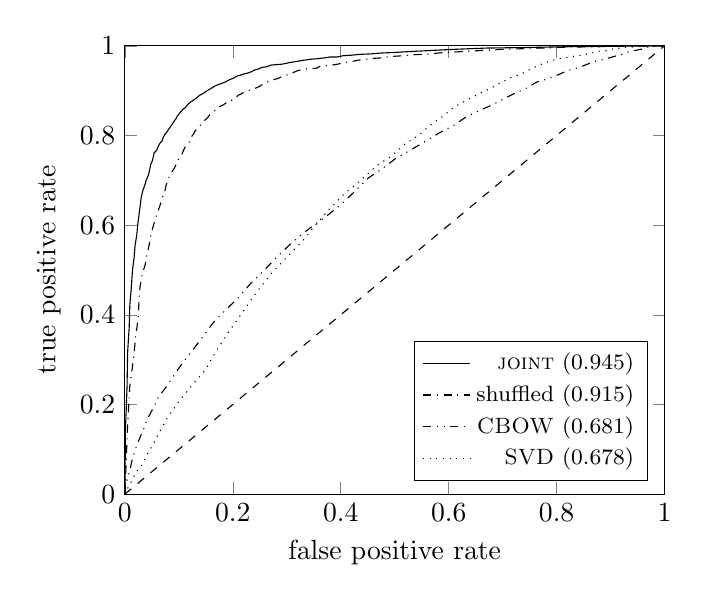
\begin{tikzpicture}
    \begin{axis}[xmin=0,xmax=1,ymin=0,ymax=1,xlabel={false positive rate},ylabel={true positive rate},legend pos=south east,legend cell align={right},legend style={font=\footnotesize}]
      \addplot [dashed,forget plot] coordinates{(0,0) (1,1)};
      \addplot [] coordinates{(0.0,0.0) (0.001,0.143) (0.004,0.240) (0.005,0.315) (0.008,0.373) (0.009,0.419) (0.012,0.463) (0.014,0.499) (0.017,0.527) (0.019,0.556) (0.022,0.578) (0.024,0.603) (0.026,0.621) (0.028,0.640) (0.030,0.660) (0.033,0.676) (0.037,0.690) (0.040,0.702) (0.044,0.713) (0.046,0.725) (0.048,0.736) (0.051,0.744) (0.053,0.754) (0.054,0.761) (0.059,0.767) (0.061,0.774) (0.065,0.783) (0.069,0.788) (0.071,0.796) (0.074,0.802) (0.078,0.808) (0.081,0.814) (0.084,0.819) (0.088,0.826) (0.092,0.833) (0.095,0.838) (0.097,0.843) (0.099,0.846) (0.102,0.851) (0.105,0.855) (0.108,0.859) (0.112,0.862) (0.116,0.868) (0.118,0.871) (0.121,0.874) (0.125,0.877) (0.128,0.880) (0.132,0.883) (0.136,0.887) (0.139,0.890) (0.144,0.893) (0.148,0.896) (0.151,0.899) (0.154,0.901) (0.157,0.903) (0.161,0.906) (0.165,0.909) (0.168,0.911) (0.174,0.914) (0.179,0.916) (0.183,0.918) (0.188,0.920) (0.190,0.922) (0.195,0.925) (0.200,0.927) (0.204,0.930) (0.209,0.933) (0.213,0.934) (0.220,0.937) (0.227,0.939) (0.234,0.942) (0.240,0.946) (0.247,0.948) (0.254,0.952) (0.262,0.953) (0.271,0.957) (0.280,0.958) (0.291,0.959) (0.299,0.961) (0.307,0.963) (0.318,0.965) (0.332,0.968) (0.345,0.970) (0.355,0.971) (0.369,0.973) (0.380,0.975) (0.393,0.975) (0.405,0.978) (0.419,0.979) (0.436,0.981) (0.456,0.982) (0.476,0.984) (0.497,0.985) (0.525,0.987) (0.558,0.989) (0.590,0.991) (0.627,0.993) (0.671,0.995) (0.732,0.996) (0.820,0.998) (1.0,1.0)}; %joint auc = 0.945
      \addplot [dash dot] coordinates{(0.0,0.0) (0.005,0.153) (0.009,0.240) (0.016,0.302) (0.020,0.352) (0.025,0.396) (0.026,0.430) (0.028,0.462) (0.032,0.489) (0.038,0.514) (0.041,0.534) (0.045,0.556) (0.048,0.576) (0.051,0.591) (0.055,0.609) (0.059,0.623) (0.063,0.637) (0.067,0.651) (0.070,0.663) (0.074,0.676) (0.076,0.687) (0.079,0.698) (0.082,0.708) (0.086,0.717) (0.090,0.724) (0.094,0.733) (0.096,0.742) (0.101,0.749) (0.106,0.759) (0.108,0.765) (0.111,0.773) (0.116,0.780) (0.119,0.785) (0.121,0.792) (0.124,0.798) (0.128,0.805) (0.130,0.810) (0.133,0.814) (0.136,0.818) (0.140,0.823) (0.144,0.828) (0.147,0.833) (0.151,0.837) (0.154,0.841) (0.157,0.846) (0.160,0.850) (0.163,0.853) (0.167,0.856) (0.169,0.860) (0.175,0.864) (0.176,0.865) (0.182,0.868) (0.188,0.873) (0.192,0.874) (0.197,0.878) (0.201,0.882) (0.204,0.884) (0.208,0.887) (0.210,0.890) (0.215,0.892) (0.218,0.895) (0.224,0.898) (0.231,0.901) (0.237,0.904) (0.243,0.906) (0.249,0.909) (0.255,0.914) (0.260,0.917) (0.265,0.920) (0.272,0.922) (0.277,0.925) (0.283,0.927) (0.291,0.931) (0.298,0.934) (0.306,0.937) (0.313,0.941) (0.321,0.945) (0.330,0.947) (0.340,0.949) (0.355,0.950) (0.361,0.954) (0.370,0.955) (0.383,0.957) (0.394,0.959) (0.408,0.963) (0.421,0.965) (0.432,0.968) (0.446,0.970) (0.460,0.972) (0.474,0.973) (0.492,0.976) (0.516,0.978) (0.535,0.980) (0.564,0.982) (0.591,0.985) (0.623,0.987) (0.653,0.989) (0.696,0.992) (0.749,0.994) (0.818,0.997) (1.0,1.0)}; %joint reshuffled auc = 0.915
      \addplot [dash dot dot] coordinates {(0.000,0.000) (0.000,0.001) (0.000,0.002) (0.001,0.006) (0.001,0.008) (0.001,0.012) (0.001,0.019) (0.002,0.025) (0.005,0.034) (0.008,0.047) (0.011,0.063) (0.014,0.079) (0.019,0.099) (0.025,0.118) (0.034,0.143) (0.041,0.166) (0.052,0.191) (0.062,0.216) (0.079,0.243) (0.092,0.267) (0.107,0.293) (0.123,0.317) (0.143,0.349) (0.164,0.383) (0.186,0.410) (0.210,0.438) (0.233,0.470) (0.257,0.498) (0.281,0.528) (0.305,0.556) (0.327,0.579) (0.355,0.604) (0.381,0.627) (0.406,0.652) (0.429,0.679) (0.451,0.705) (0.478,0.727) (0.501,0.748) (0.530,0.768) (0.557,0.787) (0.583,0.806) (0.610,0.823) (0.633,0.842) (0.656,0.855) (0.682,0.869) (0.701,0.881) (0.724,0.895) (0.745,0.906) (0.763,0.919) (0.783,0.926) (0.804,0.936) (0.821,0.945) (0.840,0.951) (0.857,0.959) (0.870,0.965) (0.885,0.969) (0.897,0.973) (0.909,0.977) (0.920,0.980) (0.929,0.985) (0.943,0.989) (0.951,0.991) (0.960,0.993) (0.966,0.996) (0.973,0.998) (0.977,0.999) (0.983,0.999) (0.987,0.999) (0.991,1.000) (0.995,1.000) (0.998,1.000) (0.999,1.000) (1.000,1.000)}; %cbow, auc = 0.681
      \addplot [dotted] coordinates{(0.000,0.000) (0.000,0.001) (0.001,0.002) (0.001,0.003) (0.002,0.004) (0.003,0.007) (0.004,0.011) (0.007,0.016) (0.009,0.022) (0.013,0.030) (0.017,0.040) (0.024,0.055) (0.033,0.067) (0.040,0.087) (0.051,0.108) (0.063,0.136) (0.079,0.171) (0.101,0.208) (0.123,0.241) (0.149,0.277) (0.169,0.319) (0.192,0.361) (0.216,0.402) (0.240,0.444) (0.269,0.489) (0.298,0.526) (0.331,0.567) (0.353,0.600) (0.378,0.635) (0.406,0.669) (0.437,0.700) (0.466,0.732) (0.496,0.756) (0.519,0.781) (0.545,0.801) (0.566,0.823) (0.587,0.841) (0.611,0.864) (0.634,0.879) (0.654,0.892) (0.676,0.904) (0.697,0.918) (0.715,0.929) (0.736,0.938) (0.753,0.949) (0.772,0.959) (0.786,0.965) (0.802,0.971) (0.818,0.974) (0.834,0.977) (0.851,0.980) (0.863,0.984) (0.878,0.988) (0.891,0.989) (0.899,0.992) (0.909,0.994) (0.920,0.995) (0.928,0.996) (0.936,0.997) (0.945,0.998) (0.950,0.999) (0.956,0.999) (0.963,0.999) (0.967,1.000) (0.972,1.000) (0.978,1.000) (0.983,1.000) (0.989,1.000) (0.994,1.000) (0.996,1.000) (0.997,1.000) (0.999,1.000) (1.000,1.000)}; %svd 2x50, auc = 0.678
      \legend{\textsc{joint} (0.945),shuffled (0.915),\textsc{CBOW} (0.681),\textsc{SVD} (0.678)} 
    \end{axis}
  \end{tikzpicture}
\caption[Receiver Operating Characterisation for Metaphor Classification]{Receiver operating characteristic plots for a selection of models, with the area under the curve for each model type indicated in the legend.}
\label{fig:metaroc}
\end{figure}

With the trade off between true and false positives in mind, Table~\ref{tab:metastats} presents precision, recall, f-score, accuracy, and Cohen's kappa scores for the same models plotted in Figure~\ref{fig:metaroc}.  The trend to notice here is that context sensitive and static models tend to favour recall over precision (and the slight preference for precision in the \textsc{joint} 400 dimensional, 5x5 word subspaces for the shuffled version of the data reported here is an anomaly, as other approaches to that data exhibit the tendency towards higher recall).  This evident enthusiasm for classifying phrases as metaphoric is a reflection of the data itself, which is slightly skewed towards metaphoric phrases, as described above and indicated in the performance of the majority class baseline, and this is reinforced by the relatively low accuracy scores for both context sensitive and static non-compositional distributional semantic models.  It is noteworthy, then, that the model described by \cite{GutierrezEA2016} actually scores better for precision than recall, suggesting it actually tends to under-predict metaphoricity.  This could perhaps be expected as a general distinction between statistical models based on unannotated data such as mine, which will arguably tend to favour a majority class, versus likewise statistical models operating on theoretically motivated mappings between representations, which have an apparent propensity for zeroing in with confidence on the properties of a compositional transformation that are indicative of metaphor---but at the expense of sometimes missing what might be considered outliers.  In the same spirit, the jumpier nature of the receiver operating characteristic plots presented by \cite{TsvetkovEA2014} is quite possibly an artefact of the decision points inherent in heuristically mapping model features from human made knowledge bases.

\begin{table}
\centering
\begin{tabular}{lrrrrr}
\hline
\ & \emph{precision} & \emph{recall} & \emph{f-score} & \emph{accuracy} & \emph{kappa} \\
\hline
\textsc{joint} & 0.879 & 0.894 & 0.886 & 0.877 & 0.753\\
shuffled & 0.873 & 0.865 & 0.862 & 0.854 & 0.678 \\
\textsc{SVD} & 0.631 & 0.794 & 0.703 & 0.641 & 0.265 \\
\textsc{CBOW} & 0.638 & 0.721 & 0.677 & 0.632 & 0.253 \\
\cite{GutierrezEA2016} & 0.842 & 0.793 & 0.817 & 0.809 & 0.618 \\
baseline & 0.535 & 1.000 & 0.697 & 0.535 & 0.000 \\
\hline
\end{tabular}
\caption[Comparative Metaphor Classification Statistics]{Full classification statistics results for the models tested here as well as the results from the original literature and the majority class (metaphor) baseline.}
\label{tab:metastats}
\end{table}

As a final point of comparison with other approaches to metaphor classification, I will return briefly to the unannotated character of my lexical representations.  One of the most powerful features of the methodology described here is its ability to build a somewhat general model of a semantic phenomenon from a sufficiently comprehensive dataset, and the strong Cohen's kappa score of the best performing subspace selection technique, which begins to approach the aforementioned inter-annotator agreement level of $\kappa = 0.80$, is a testament to this.  Following an analysis of the specific geometry of metaphor in the next section, Section~\ref{sec:genaphor} will assess the ability of my methodology to generalise even further from this data to a broader range of metaphors and to moreover move from classification to gradation based on observations of merely binary judgements of metaphoricity.  For now, I simply note that it is remarkable that data about nothing more than the way that words tend to be collocated can, with the aid of a mechanism for contextualisation, reveal so much about the nature of the semantic relationship between the lexical components of an previously unseen phrase.

\subsection{The Geometry of Metaphor}
In this section, I will explore the geometric features which prove most productive in the classification of metaphor.  As with relatedness and similarity in the previous chapter, I begin by examining the capacity of independent features to predict metaphor.  Rather than a proper logistic regression involving multiple independent variables fed into a non-linear function, this analysis amounts to choosing a cut-off point in terms of the value of each feature separating literal and metaphoric phrases in the subspaces which an analysis of their corresponding word-vectors delineate.  So the f-scores reported in Table~\ref{tab:ind-metaphor} can be understood as indicating the degree to which the values of a given geometric feature separate the dataset into distinct categories corresponding to human judgements of metaphoricity.

\begin{table}
\centering
\begin{tabular}{lr|lr|lr}
\hline
\multicolumn{2}{c}{\textsc{joint}} & \multicolumn{2}{c}{\textsc{indy}} & \multicolumn{2}{c}{\textsc{zipped}} \\
\hline
$\mu(A,B)$ & 0.787 & $C$ & 0.767 & $\mu(A,B)$ & 0.788 \\
$C$ & 0.771 & $C/M$ & 0.749 & $C$ & 0.771 \\
$\mu(A,B)/M$ & 0.764 & $\angle AMB$ & 0.747 & $\mu(A,B)/M$ & 0.769 \\
$\angle COX$ & 0.762 & $C/X$ & 0.746 & $X$ & 0.767 \\
$X$ & 0.762 & $\mu(A,B)$ & 0.734 & $\mu(A,B)/X$ & 0.759 \\
\hline
\end{tabular}
\vfill
\begin{tabular}{lr|lr}
\multicolumn{2}{c}{\textsc{adjective}} & \multicolumn{2}{c}{\textsc{noun}} \\
\hline
$\mu(A,B)/M$ & 0.745 & $\mu(A,B)$ & 0.756 \\
$\overline{AC}:\overline{BC}$ & 0.736 & $C$ & 0.747 \\
$\overline{AC}/\overline{BC}$ & 0.734 & $\mu(A,B)/X$ & 0.728 \\
$\mu(A,B)/X$ & 0.732 & $\mu(A,B)/M$ & 0.721 \\
$\angle ACB$ & 0.730 & $C/X$ & 0.721 \\
\hline
\end{tabular}
\caption[Top Independent Features for Metaphor Classification]{Independent f-scores from the metaphor classification data for top five features of each subspace type for 5x5 word co-occurrence window, 400 dimension subspaces.}
\label{tab:ind-metaphor}
\end{table}

%\begin{table}
%\centering
%\begin{tabular}{lr|lr|lr|lr|lr}
%\hline
%\multicolumn{2}{c}{\textsc{joint}} & \multicolumn{2}{c}{\textsc{indy}} & \multicolumn{2}{c}{\textsc{zipped}} & \multicolumn{2}{c}{\textsc{adjective}} & \multicolumn{2}{c}{\textsc{noun}} \\
%\hline
%$\mu(A,B)$ & 0.785 & $C$ & 0.767 & $\mu(A,B)$ & 0.788 & $\mu(A,B)/M$ & 0.744 & $\mu(A,B)$ & 0.756 \\
%$C$ & 0.768 & $\angle AMB$ & 0.749 & $\mu(A,B)/M$ & 0.771 & $\overline{AC}:\overline{BC}$ & 0.737 & $C$ & 0.745 \\
%$\mu(A,B)/M$ & 0.764 & $C/M$ & 0.748 & $X$ & 0.769 & $\mu(A,B)/C$ & 0.736 & $\mu(A,B)/X$ & 0.728 \\
%$X$ & 0.763 & $C/X$ & 0.747 & $C$ & 0.767 & $\mu(A,B)/X$ & 0.733 & $\mu(A,B)/M$ & 0.722 \\
%$\mu(A,B)/X$ & 0.759 & $\mu(A,B)$ & 0.733 & $\mu(A,B)/X$ & 0.762 & $\angle ACB$ & 0.732 & $C/X$ & 0.721 \\
%\hline
%\end{tabular}
%\caption[Top Independent Features for Metaphor Classification with Unseen Adjectives]{Independent f-scores from the metaphor classification data for top five features of each subspace type for 5x5 word co-occurrence window, 400 dimension subspaces with models tested on adjectives not observed in training.}
%\label{tab:ind-metaphor}
%\end{table}

The scores themselves reflect the trend observed in Table~\ref{tab:metaphor} and~\ref{tab:categoraphor}: the \textsc{joint} and \textsc{zipped} subspaces produce features that are particulary good at classifying metaphor, with a decrease in performance in the \textsc{indy} subspaces and then another step down in the single-word subspaces.  None of the scores themselves come close to the levels of discrimination achieved by the models learned from full feature vectors, with the difference between the performance of the best feature for the \textsc{joint} technique and that of the corresponding full featured space somehwat significant with $p = .006$.  In terms of the actual features indicated by this analysis, two in particular figure prominently in one way or another, namely, the mean of the word-vector norms $\mu(A,B)$ and the norm of the central-vector $C$.  In the first instance, the role of the relationship between word-vectors and the origin of the spaces that their salient co-occurrence dimensions delineate is once again reflective of the preliminary findings on conceptual geometry described in Chapter~\ref{sec:pof}, where norm was seen to be an effective mechanism for defining a region of conceptual constituency.  In the case of the distance of the central vector from the origin, the emergence of this feature, as well of the appearance of the norms $M$ and $X$ as components of various strongly predictive tendencies, indicate that here, as with similarity in the previous chapter, characteristics of dimensions outside of the situation of any particular word-vector along them might be in themselves indicative of metaphor: some words might simply be more likely to co-occur in the context of metaphoric language, and co-occurrence statistics should provide a handle for examining this tendency.

To further delve into the statistical geometry of metaphor, and in line with the results on relatedness and similarity described in the previous chapter, I once again search the state space of possible combinations of features to find the optimal feature vector for classifying metaphor in context sensitive subspaces.  This is again treated as a beam search problem, though the search space expanded at each level of the search tree is here limited to the top 500 combinations of features given the larger size of the data being modelled.  Table~\ref{tab:metatures} presents the optimal seven feature combinations discovered for the 5x5 word window, 400 dimensional \textsc{joint} subspaces based on both a standard ten-fold cross-validation and the version of the data shuffled in order to test on data not observed in each training phase.  The f-scores achieved by these combinations of features, reported next to the respective labels at the top of the table, indicate a marginal decrease in the overall performance as compared to the full featured models of subspaces, but the results are still strong.

\begin{table}
\centering
\begin{tabular}{llr}
\hline
& \multicolumn{1}{c}{10-fold ($f = 0.869$)} & \multicolumn{1}{c}{shuffled ($f = 0.830$)} \\
\hline
& \multicolumn{2}{c}{\textsc{distances}} \\
word-vectors& - & - \\
generic vectors & $M = -1.448$ & - \\
\hline
& \multicolumn{2}{c}{\textsc{angles}} \\
word-vectors & $\angle ACB = -0.775$ & - \\
normalised & - & - \\
generic vectors & $\angle COX = -1.618$ & $-0.271 = \angle COM$  \\
& $\angle COM = 0.974$ & $0.045 = \angle MOX$ \\
\hline
& \multicolumn{2}{c}{\textsc{means}} \\
word-vectors & $\mu(\overline{AM},\overline{BM}) = -1.124$ & $-1.007 = \mu(\overline{AC},\overline{BC})$ \\
normalised & - & - \\
\hline
& \multicolumn{2}{c}{\textsc{ratios}} \\
word-vectors & - & $0.492 = \overline{AM}:\overline{BM}$ \\
& & $-0.620 = \overline{AX}:\overline{BX}$ \\
normalised & - & $-0.168 = \overline{A'C'}:\overline{B'C'}$ \\
\hline
& \multicolumn{2}{c}{\textsc{fractions}} \\
word-vectors & $\overline{AC}/\overline{BC} = 0.325$ & - \\
generic vectors & $M/X = 1.305$ & $0.252 = A/B$ \\
\hline
\end{tabular}
\caption[Most Predictive Feature Vectors for Metaphor Classification]{The seven most predictive features for metaphor classification, compared between ten-fold and sight-unseen cross-validation of logistic regression on statistics extrapolated from 5x5 word window, 400 dimensional \textsc{joint} subspaces.}
\label{tab:metatures}
\end{table}

Angles between generic vectors, which were already evident as independently predictive features in Table~\ref{tab:ind-metaphor}, have a strong effect here, with the strong negative correlation of $\angle COX$ in the ten-fold cross-validation in particular suggesting that maximal values tend to be relatively similar across dimensions jointly selected by literal adjective-noun combinations, pulling the line of $X$ closer to the centroid described by $C$.  To put this differently, as pairs become more metaphoric, they tend to also become less consistent in the type of dimension that they co-select, as evidenced in the increasing variance in the maximum values of these dimensions.  Perhaps the most interesting thing to observe here, though, is the strong correlation between ratios of word-vector to generic vector distances in the case of the version of the data shuffled to test on unseen adjectives, but not in the case of the stratified cross-validation.  The positive correlation with the balance of the distances from the word-vectors to the mean vector $M$ means that subspaces where the word-vectors have a relatively even relationship to the weighted centre are, in fact, more metaphoric (and their relationship to the maximum vector is comparatively less balanced, with this vector in turn being less central to the space per the observations regarding $\angle COX$).  But more generally, it is noteworthy that the balance between word vectors and generic vectors is informative about metaphoricity specifically in models tested on unseen adjectives: this balance is in effect a projection into space of quotients of joint probabilities of observing words and co-occurrence terms divided by the typical or maximal probabilities of being observed with the co-occurrence terms, and from it we can infer that these quotients are generally predictive of metaphor in context, even without word-specific training data.

Figure~\ref{fig:metaspaces} presents visualisations by way of three dimensional projections of word-vectors and generic vectors from 400 dimensional \textsc{joint} subspaces selected from the 5x5 word window base space.\footnote{These projections have been rendered using the same regression technique as applied to the images for related word pairs in the previous section, but the coordinates of $X$ have been divided by 1.5 instead of 2.}  In the example of the uncontroversially literal phrase \emph{sweet watermelon}, the word-vectors are characteristically far from the origin and close to one another, corresponding to the predictivity of $\mu(A,B)$ in particular.  At the other extent of the spectrum, the highly metaphoric phrase \emph{bitter letter} is characterised by a dropping of the word-vectors and a widening of the angle between them; the generic vectors, meanwhile, are now further from the origin relative to the word-vectors that select the subspace and, at the same time, draw closer to one another in particular at the normalised layer of the subspace.  But most interestingly, at a relatively neutral point, occupied by the intriguingly ambiguous phrase \emph{warm country}, which the logistic regression trained on these subspaces assigned a score of close to 0.5, there is actually evidence of an intermediary widening out of the overall array of points even as the word-vectors remain fairly far from the origin.

\begin{figure}
\footnotesize
\begin{subfigure}{0.3\textwidth} % sour - sauce
\centering
  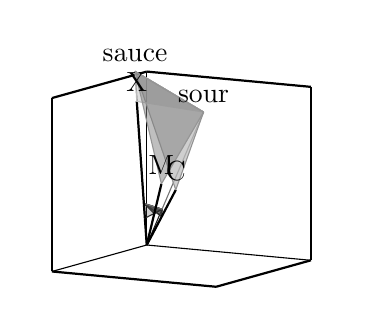
\begin{tikzpicture}
    \def\varA{(56.2720,60.1719,75.2389)};
    \def\varB{(73.7099,36.8692,94.6119)};
    \def\varC{(33.4740,33.4737,33.4739)};
    \def\varM{(36.1929,28.0423,36.1855)};
    \def\varX{(117.9619,63.2478,89.8183)};
    \def\varAN{(15.1308,16.1795,20.2308)};
    \def\varBN{(17.6235,8.8151,22.6210)};
    \def\varCN{(17.3206,17.3204,17.3205)};
    \def\varMN{(18.6056,14.4156,18.6017)};
    \def\varXN{(21.9544,11.7713,16.7165)};
    \def\nodA{56.2720,60.1719,75.2389};
    \def\nodB{73.7099,36.8692,94.6119};
    \def\nodC{33.4740,33.4737,33.4739};
    \def\nodM{36.1929,28.0423,36.1855};
    \def\nodX{117.9619,63.2478,89.8183};
    \begin{axis}[scale = 0.6,axis line style=white,view={120}{10},xmin=0,xmax=100,ymin=0,ymax=100,zmin=0,zmax=100,colormap/blackwhite,ticks=none]
      \addplot3[color=black,thick] coordinates {(0,0,80) (0,80,80)};
      \addplot3[color=black,thick] coordinates {(0,0,80) (80,0,80)};
      \addplot3[color=black,thick] coordinates {(0,80,0) (0,80,80)};
      \addplot3[color=black,thick] coordinates {(0,80,0) (80,80,0)};
      \addplot3[color=black,thick] coordinates {(80,0,0) (80,0,80)};
      \addplot3[color=black,thick] coordinates {(80,0,0) (80,80,0)};
      \addplot3[color=black] coordinates {(0,0,0) (0,0,80)};
      \addplot3[color=black] coordinates {(0,0,0) (0,80,0)};
      \addplot3[color=black] coordinates {(0,0,0) (80,0,0)};
      \addplot3[patch,patch type=triangle,color=gray,fill opacity=0.0] coordinates {(0.0,0.0,0.0) \varCN \varAN};
      \addplot3[patch,patch type=triangle,color=gray,fill opacity=0.0] coordinates {(0.0,0.0,0.0) \varCN \varBN};
      \addplot3[patch,patch type=triangle,color=darkgray,fill opacity=0.75] coordinates {\varCN \varAN \varBN};
      \addplot3[patch,patch type=triangle,color=darkgray,fill opacity=0.5] coordinates {\varMN \varAN \varBN};
      \addplot3[patch,patch type=triangle,color=darkgray,fill opacity=0.25] coordinates {\varXN \varAN \varBN};
      \addplot3 [color=black,thick] coordinates {(0,0,0) \varCN};
      \addplot3 [color=black,thick] coordinates {(0,0,0) \varXN};
      \addplot3 [color=black,thick] coordinates {(0,0,0) \varMN};
%      \addplot3[opacity = 0.1,surf,z buffer = sort,samples = 21,variable = \u,variable y = \v,domain = 0:90,y domain = 0:90,]
%    ({1*cos(u)*sin(v)}, {1*sin(u)*sin(v)}, {1*cos(v)});
      \addplot3 [patch,patch type=rectangle,color=lightgray,fill opacity=0.0] coordinates{\varAN \varA \varB \varBN
};
      \addplot3 [color=black,thick] coordinates {\varCN \varC};
      \addplot3 [color=black,thick] coordinates {\varXN \varX};
      \addplot3 [color=black,thick] coordinates {\varMN \varM};
      \addplot3 [patch,patch type=triangle,color=lightgray,fill opacity=0.75] coordinates{\varA \varC \varB};
      \addplot3 [patch,patch type=triangle,color=gray,fill opacity=0.25] coordinates{\varA \varX \varB};
      \addplot3 [patch,patch type=triangle,color=gray,fill opacity=0.5] coordinates{\varA \varM \varB};
      \node [anchor=south] at (axis cs: \nodA) {sour};
      \node [anchor=south] at (axis cs: \nodB) {sauce};
      \node [anchor=south] at (axis cs: \nodC) {C};
      \node [anchor=south] at (axis cs: \nodX) {X};
      \node [anchor=south] at (axis cs: \nodM) {M};
    \end{axis}
  \end{tikzpicture}
\caption*{\footnotesize \emph{literal: sweet watermelon}}
\end{subfigure}
\hfill
\begin{subfigure}{0.3\textwidth} % warm - country
\centering
  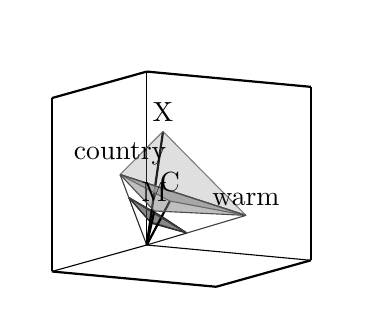
\begin{tikzpicture}
\def\varA{-8.639,51.611,50.881};
    \def\varA{(28.1002,64.5545,23.6443)};
    \def\varB{(25.5857,1.7784,36.5694)};
    \def\varC{(26.7296,26.7293,26.7296)};
    \def\varM{(33.9479,23.3011,22.9391)};
    \def\varX{(106.0249,69.1555,74.6834)};
    \def\varAN{(11.3507,26.0758,9.5508)};
    \def\varBN{(17.1844,1.1944,24.5615)};
    \def\varCN{(17.3206,17.3204,17.3206)};
    \def\varMN{(21.6073,14.8308,14.6004)};
    \def\varXN{(21.6416,14.1159,15.2442)};
    \def\nodA{28.1002,64.5545,23.6443};
    \def\nodB{25.5857,1.7784,36.5694};
    \def\nodC{26.7296,26.7293,26.7296};
    \def\nodM{33.9479,23.3011,22.9391};
    \def\nodX{106.0249,69.1555,74.6834};
    \begin{axis}[scale = 0.6,axis line style=white,view={120}{10},xmin=0,xmax=100,ymin=0,ymax=100,zmin=0,zmax=100,colormap/blackwhite,ticks=none]
      \addplot3[color=black,thick] coordinates {(0,0,80) (0,80,80)};
      \addplot3[color=black,thick] coordinates {(0,0,80) (80,0,80)};
      \addplot3[color=black,thick] coordinates {(0,80,0) (0,80,80)};
      \addplot3[color=black,thick] coordinates {(0,80,0) (80,80,0)};
      \addplot3[color=black,thick] coordinates {(80,0,0) (80,0,80)};
      \addplot3[color=black,thick] coordinates {(80,0,0) (80,80,0)};
      \addplot3[color=black] coordinates {(0,0,0) (0,0,80)};
      \addplot3[color=black] coordinates {(0,0,0) (0,80,0)};
      \addplot3[color=black] coordinates {(0,0,0) (80,0,0)};
      \addplot3[patch,patch type=triangle,color=gray,fill opacity=0.0] coordinates {(0.0,0.0,0.0) \varCN \varAN};
      \addplot3[patch,patch type=triangle,color=gray,fill opacity=0.0] coordinates {(0.0,0.0,0.0) \varCN \varBN};
      \addplot3[patch,patch type=triangle,color=darkgray,fill opacity=0.75] coordinates {\varCN \varAN \varBN};
      \addplot3[patch,patch type=triangle,color=darkgray,fill opacity=0.5] coordinates {\varMN \varAN \varBN};
      \addplot3[patch,patch type=triangle,color=darkgray,fill opacity=0.25] coordinates {\varXN \varAN \varBN};
      \addplot3 [color=black,thick] coordinates {(0,0,0) \varCN};
      \addplot3 [color=black,thick] coordinates {(0,0,0) \varXN};
      \addplot3 [color=black,thick] coordinates {(0,0,0) \varMN};
%      \addplot3[opacity = 0.1,surf,z buffer = sort,samples = 21,variable = \u,variable y = \v,domain = 0:90,y domain = 0:90,]
%    ({1*cos(u)*sin(v)}, {1*sin(u)*sin(v)}, {1*cos(v)});
      \addplot3 [patch,patch type=rectangle,color=lightgray,fill opacity=0.0] coordinates{\varAN \varA \varB \varBN
};
      \addplot3 [color=black,thick] coordinates {\varCN \varC};
      \addplot3 [color=black,thick] coordinates {\varXN \varX};
      \addplot3 [color=black,thick] coordinates {\varMN \varM};
      \addplot3 [patch,patch type=triangle,color=lightgray,fill opacity=0.75] coordinates{\varA \varC \varB};
      \addplot3 [patch,patch type=triangle,color=gray,fill opacity=0.25] coordinates{\varA \varX \varB};
      \addplot3 [patch,patch type=triangle,color=gray,fill opacity=0.5] coordinates{\varA \varM \varB};
      \node [anchor=south] at (axis cs: \nodA) {warm};
      \node [anchor=south] at (axis cs: \nodB) {country};
      \node [anchor=south] at (axis cs: \nodC) {C};
      \node [anchor=south] at (axis cs: \nodX) {X};
      \node [anchor=south] at (axis cs: \nodM) {M};
    \end{axis}
  \end{tikzpicture}
\caption*{\footnotesize \emph{neutral: warm country}}
\end{subfigure}
\hfill
\begin{subfigure}{0.3\textwidth} % bitter - letter
\centering
  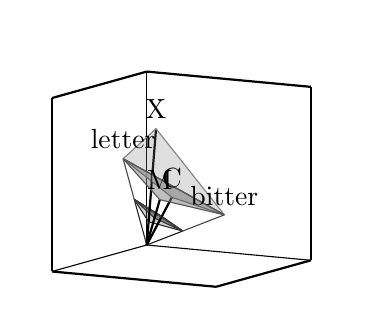
\begin{tikzpicture}
    \def\varA{(27.7652,53.8416,22.8974)};
    \def\varB{(33.0985,7.5929,45.5444)};
    \def\varC{(28.9808,28.9805,28.9808)};
    \def\varM{(33.1872,25.5252,28.2293)};
    \def\varX{(109.8650,67.9613,76.3988)};
    \def\varAN{(12.8618,24.9413,10.6069)};
    \def\varBN{(17.4783,4.0096,24.0506)};
    \def\varCN{(17.3206,17.3204,17.3206)};
    \def\varMN{(19.7168,15.1648,16.7713)};
    \def\varXN{(21.9604,13.5845,15.2710)};
    \def\nodA{27.7652,53.8416,22.8974};
    \def\nodB{33.0985,7.5929,45.5444};
    \def\nodC{28.9808,28.9805,28.9808};
    \def\nodM{33.1872,25.5252,28.2293};
    \def\nodX{109.8650,67.9613,76.3988};
    \begin{axis}[scale = 0.6,axis line style=white,view={120}{10},xmin=0,xmax=100,ymin=0,ymax=100,zmin=0,zmax=100,colormap/blackwhite,ticks=none]
      \addplot3[color=black,thick] coordinates {(0,0,80) (0,80,80)};
      \addplot3[color=black,thick] coordinates {(0,0,80) (80,0,80)};
      \addplot3[color=black,thick] coordinates {(0,80,0) (0,80,80)};
      \addplot3[color=black,thick] coordinates {(0,80,0) (80,80,0)};
      \addplot3[color=black,thick] coordinates {(80,0,0) (80,0,80)};
      \addplot3[color=black,thick] coordinates {(80,0,0) (80,80,0)};
      \addplot3[color=black] coordinates {(0,0,0) (0,0,80)};
      \addplot3[color=black] coordinates {(0,0,0) (0,80,0)};
      \addplot3[color=black] coordinates {(0,0,0) (80,0,0)};
      \addplot3[patch,patch type=triangle,color=gray,fill opacity=0.0] coordinates {(0.0,0.0,0.0) \varCN \varAN};
      \addplot3[patch,patch type=triangle,color=gray,fill opacity=0.0] coordinates {(0.0,0.0,0.0) \varCN \varBN};
      \addplot3[patch,patch type=triangle,color=darkgray,fill opacity=0.75] coordinates {\varCN \varAN \varBN};
      \addplot3[patch,patch type=triangle,color=darkgray,fill opacity=0.5] coordinates {\varMN \varAN \varBN};
      \addplot3[patch,patch type=triangle,color=darkgray,fill opacity=0.25] coordinates {\varXN \varAN \varBN};
      \addplot3 [color=black,thick] coordinates {(0,0,0) \varCN};
      \addplot3 [color=black,thick] coordinates {(0,0,0) \varXN};
      \addplot3 [color=black,thick] coordinates {(0,0,0) \varMN};
%      \addplot3[opacity = 0.1,surf,z buffer = sort,samples = 21,variable = \u,variable y = \v,domain = 0:90,y domain = 0:90,]
%    ({1*cos(u)*sin(v)}, {1*sin(u)*sin(v)}, {1*cos(v)});
      \addplot3 [patch,patch type=rectangle,color=lightgray,fill opacity=0.0] coordinates{\varAN \varA \varB \varBN
};
      \addplot3 [color=black,thick] coordinates {\varCN \varC};
      \addplot3 [color=black,thick] coordinates {\varXN \varX};
      \addplot3 [color=black,thick] coordinates {\varMN \varM};
      \addplot3 [patch,patch type=triangle,color=lightgray,fill opacity=0.75] coordinates{\varA \varC \varB};
      \addplot3 [patch,patch type=triangle,color=gray,fill opacity=0.25] coordinates{\varA \varX \varB};
      \addplot3 [patch,patch type=triangle,color=gray,fill opacity=0.5] coordinates{\varA \varM \varB};
      \node [anchor=south] at (axis cs: \nodA) {bitter};
      \node [anchor=south] at (axis cs: \nodB) {letter};
      \node [anchor=south] at (axis cs: \nodC) {C};
      \node [anchor=south] at (axis cs: \nodX) {X};
      \node [anchor=south] at (axis cs: \nodM) {M};
    \end{axis}
  \end{tikzpicture}
\caption*{\footnotesize \emph{metaphoric: bitter letter}}
\end{subfigure}
\caption[Metaphors In Space]{Three dimensional projections of word-vectors and generic vectors in subspaces for pairs at the extents and in the middle of the literal-metaphorical spectrum, taken from 5x5 word window, 400 dimensional subspaces selected using the \textsc{joint} technique.}
\label{fig:metaspaces}
\end{figure}

The exciting thing about this last observation is that it suggests that, rather than existing on a linear or even monotonic scale, metaphor may itself actually be a multi-dimensional phenomenon, with a characteristic particular to highly ambiguous word combinations that is to some extent separate from the statistical features of straightforward literalness and clear cut metaphoricity.  The broad arrangement of word-vectors in space engendered by the contextualisation of the phrase \emph{warm country}, in contrast to the relatively tight relationship of the generic vectors, can be interpreted as revealing an uncertainty regarding the semantic properties being transferred in this small composition, corresponding to a drifting of the word-vectors and a contracting of the generic vectors across the jointly selected co-occurrence profile.  Here, once again, the statistical geometry of a subspace can be productively mapped to a theoretical statement about the nature of a semantic phenomenon as characterised by a selectively contextual and quantitative representation of observations about the way that words are used, by and large outside of any strong preconditions symbolically encoded in the computational framework.

\subsection{Generalising the Model} \label{sec:genaphor}
One of the interesting things about feature-based classification is that there is typically an inherent commitment to degree of class membership, even when the training data used to build a model is simply binary.  This is true of any model which uses, for instance, a logistic regression technique for determining class, as there is a cut-off point along the spectrum of model output and a corresponding proximity to that point for any given sample, and it is especially obvious when the features of the model are actually geometrical measures.  In this section, I will apply the models learned from the the \cite{GutierrezEA2016} data to another dataset designed to assess metaphor as a matter of degree rather than simply as a binary situation, and a dataset that additionally deals with a different type of metaphor in terms of composition.  The question explored here is whether the geometric features of context specific distributional semantic analysis of word-vectors will provide binary classification models with adequate information for projecting metaphoricity along a continuous scale.

The data used for this experiment was originally reported by \cite{JankowiakEA2015}, and was used to train a model based on an earlier version of methodology as described by \cite{AgresEA2016}.  This data consists of 228 predicate-object word pairs selected to cover three degrees of metaphor, consisting of literal pairs such as \emph{announce willingness}, conventionally metaphoric pairs such as \emph{cut pollution}, and novel metaphors such as \emph{smell excuses}.  102 human participants provided metaphoricity scores on a seven point Likert scale, and the average scores were compiled into the dataset that will used to test models learned from the geometric features output by my context sensitive methodology.\footnote{Studies were also conducted to gather ratings for \emph{familiarity} and \emph{meaningfulness}, but those ratings will not be modelled in this thesis.}  Specifically, I will experiment with two different classification model techniques.  In the first instance, I will take the output of the logistic regression described above, trained on the \cite{GutierrezEA2016} data, as assigning probabilities to the metaphoricity of an input word pair, and I will in turn measure the degree to which these probabilities correlate with the degree of metaphoricity collectively assigned by human raters.  In the second instance, I'll use the binary metaphor classification data to train a support vector machine.\footnote{This is implemented using the python scikit-learn \texttt{SVC} module.}  Applying a radial basis function kernel, I analyse the correlation between distance from the discriminatory hyperplane and the human ratings.  In both cases, and in line with results reported in the previous chapter, Spearman's correlations are the unit of analysis.

\begin{table}
\centering
\begin{tabular}{lrrrrrr}
\hline
\emph{features} & 1 & 3 & 5 & 7 & 9 & full \\
\hline
& \multicolumn{6}{c}{\emph{logistic regression}} \\
\textsc{joint} & 0.368 & 0.355 & 0.033 & 0.085 & 0.279 & -0.033 \\
\textsc{adjective} & -0.377 & 0.355 & 0.044 & 0.513 & 0.511 & 0.335 \\
\hline
& \multicolumn{6}{c}{\emph{support vector machine}} \\
\textsc{joint} & 0.352 & 0.359 & 0.042 & 0.045 & 0.243 & 0.158 \\
\textsc{adjective} & -0.170 & 0.247 & -0.021 & 0.407 & 0.418 & 0.236 \\
\hline
\end{tabular}
\caption[Scoring Metaphoricity Based On Classification Data]{Spearman's correlation with human verb-noun metaphoricity scales judgements based on logistic regression and support vector machine models trained on adjective-noun classification data, taking feature vectors of various lengths as independent variables.}
\label{tab:verblearn}
\end{table}

Table~\ref{tab:verblearn} presents results for both modelling techniques, focussing on features extrapolated from 5x5 word window, 400 dimensional subspaces using the \textsc{joint} approach and through an analysis on the adjective in each word-pair from the input data.  Feature vectors of various lengths, picking the optimal geometric features for each dimensional selection technique, are used to feed input to each model.  In terms of the models trained on features from \textsc{joint} subspaces, there is a clear trend towards strong performance with one or three features, weaker performance with five or seven features, stronger performance again with nine features, and then a drop-off again in the full featured space.  The relatively low performance with the full set of features is not particularly surprising: there is clearly an encroaching incidence of generalisation error here as the models become flooded with data about various and certainly collinear statistical features of contextual geometry.  At the shallow end of the feature selection parameters, on the other hand, the single measure $\mu(A,B)$ (per Table~\ref{tab:ind-metaphor}) once again points to the efficacy of word-vector norm as a predictive characteristic of contextualised co-occurrence subspaces.

The really remarkable outcome here, though, is the very strong performance of the models learned from the top seven and nine features extracted from subspaces selected by PMI values of the adjective word-vectors alone.  This is particularly interesting given that the data being tested actually consists of a different type of grammatical relationship, namely, predicate-object pairs.  It would seem, then, that the co-occurrence dimensions most salient to either verbs or adjectives generate a geometry in which their relationship to potential arguments can play out in similar ways in terms of the metaphoricity inherent in the semantic context: the interaction between the selecting vector, the noun-vector, and the generic vectors translates from one type of composition to another in an isomorphic way.  This explantion, including the claim that the mapping of predictive features from one type of metaphor to the other is to a large extent isomorphic, is supported by the particularly strong performance of the logistic regression at seven and nine dimensions, where the logistic function takes a polynomial with coefficients learned in the training phase as direct input.  The more complex non-linearity afforded by the support vector machine appears to actually somewhat confound the mapping from verb-noun to adjective-noun phrases---though the difference between the correlations at nine dimensions is not statistically significant at $p = .104$ based on a Fisher r-to-z transformation.

The one area where a support vector machine provides a clear improvement in performance is in the full dimensional models extrapolated from \textsc{joint} subspaces.  In this case, it would seem that the radial basis function classification actually does a better job of avoiding the overfitting in a higher dimensional feature space.  But, putting questions of model choice aside, there is clear evidence here for the generality of the contextual geometry of metaphor, and also a strong case for the appropriateness of machine learning techniques for providing an appropriate mechanism for the computational manipulation of co-occurrence information to build a more nuanced model of degree of metaphor based on relatively rudimentary classification data.  Crucially, it is the context sensitivity of my methodology that facilitates the exploration of a multi-dimensional feature space in which the non-linear nuances of this particular semantic phenomenon can be discovered; a model providing a singular static relationship between lexical representations could not offer the context specific underpinning for generating a geometry replete with interpretable statistical features.  Finally, there are signs here to invite further research, and indeed some grounds for hoping that a context sensitive approach might have the scope for handling more sophisticated tasks such as metaphor interpretation and generation.

\section{An Experiment on Coercion}
In this section, I will apply my methodology to the classification of a phenomenon closely related to metaphor, namely, \emph{semantic type coercion}, by which the semantic type of a word is shifted through its interaction with another word: in the cases examined here, verbs that select for a particular semantic type will be seen to coerce nouns from one conceptual category to another by taking those nouns as arguments.  So, for instance, in phrases like \emph{denied wrongdoing} or \emph{heard footsteps}, the nouns in play are standing in for a conceptually relevant but different type of noun, and the literal versions of these phrases would go something like \emph{denied committing wrongdoing} or \emph{heard the sound of footsteps}, where the verbs select arguments of types along the lines of \textsc{activity} and \textsc{perception} respectively.  This phenomenon is often referred to as \emph{logical metonymy}, identifying it as a subspecies of the more general figurative phenomenon metonymy by which a thing is denoted by a conceptually related lexical representation.

Coercion is one of the semantic phenomena targeted by \citepos{Pustejovsky1995} theory of a \emph{generative lexicon}, by which nouns are semantically modelled as having a \emph{qualia structure} which maps out the way that a thing relates to itself, the world, and the agents interacting with it in that world on four different levels of abstraction, with the general objective of arriving at ``a model of meaning in language that captures the means by which words can assume a potentially infinite number of senses in context, while limiting the number of senses actually stored in the lexicon,'' (ibid, p. 104).  In terms of coercion, qualia provide the basis for a process of \emph{projection} by which a variety of semantic types can be extracted from a complex type (or a \emph{dot object} in Pustejovsky's lingo) in order to fulfil the typing requirements of a predicate in open ended ways.  The model that emerges here -- one built on dynamically interactive lexical semantic representations contingent on some sort of general conceptual context -- begins to look like the general linguistic stance that has motivated my own methodology.

This theoretical commitment suggests a schematic by which a symbol manipulating system might begin to get a handle on productive and context sensitive lexical representations of things in the world.  To this end, \cite{JezekEA2010} have described an ontology based on a computational analysis of co-occurrence patterns designed to facilitate the modelling of what is ultimately a sliding scale of statistically enhanced semantic representations, or ``shimmering lexical sets,'' (ibid, p. 19), as the authors put it.  Applying a similar notion that coercion is probabilistic rather than discreet, \cite{LapataEA2003} use co-occurrence statistics to try to predict the verbs which, in the role of for instance participles, successfully resolve instances of coercion.  And, under the rubric of \emph{logical metonymy}, \cite{ShutovaEA2013b} expand upon the work of \citeauthor{LapataEA2003} by extracting verb senses from WordNet to build a class based model, to some extent recapitulating the categorical distinctions that characterise many theoretical approaches to coercion.  The motivation behind this last system is the apt observation that, in the case of coercion, ``humans are capable of interpreting these phrases using their world knowledge and contextual information,'' \citep[][11:2]{ShutovaEA2013b}.

Returning to the theoretical issues regarding grammaticality raised earlier in this chapter, the analysis of coercion within the framework of the generative lexicon points to something more like a graduated typology, sliding from specific instances of processes, things, and the like to more general conceptual categories and finally to entire classes of words.  As \cite{Langacker1991} has pointed out, there is a lurking ambiguity in grammatical class distinctions, with various conceptual schema existing in any natural language for moving between classes: so, to borrow an example from Langacker, phonological and symbolic dynamics facilitate a conceptually coherent progression from \emph{sharp} to \emph{sharpen} to \emph{sharpener}, and the rules that are extrapolated as an explanatory framework for such transitions are just a way of systematising the cognitive networks that underpin this linguistic phenotype.\footnote{\citepos{Wittgenstein1953} quip regarding ``grammatical fictions,'' (ibid, \P 307) also comes to mind.}  And as \cite{BriscoeEA} point out in their probabilistic account of coercion, selectional preferences are at least to a certain extent conditioned by factors involving word frequency, suggesting that there could be grounds for a distributional mechanism for modelling semantic shifting.

With this in mind, my hypothesis is that, as with metaphor in the previous section, a syntactically neutral statistical model with a context generating capacity should be able to capture the way in which, in the case of argument type coercion, a predicate specifies some conceptual contingency of the coerced object in order to accommodate its selectional preference.  The purpose of this set of experiments (an early version of which is reported in \cite{McGregorEA2017}) is to test this broad hypothesis, and to explore the particular statistical features of co-occurrence which afford appropriate contextualisations.  This will serve, to a certain extent, to address a question raised by \cite{PustejovskyEA2008}, who illustrate some of the difficulties inherent in extracting typological structure from a distributional analysis of a large-scale corpus.  The point made there is that ``generative mechanisms in the semantics, such as coercion, modulate meanings in context and allow words to behave distributionally in unexpected ways with respect to their selectional properties,'' (ibid, p. 209).  Those authors show how a model involving a dynamic between a statistical approach such as a distributional semantic model and a theoretical structure such as the generative lexicon can accommodate some of this unexpectedness.  My goal in the following experiments is to explore the extent to which a context sensitive approach to distributional semantics can, without the structure of a symbolic formalism or pre-formulated grammatical or typological annotations, address the pertinent theoretical issues raised by the kind of analysis offered by \citeauthor{PustejovskyEA2008}.

\subsection{Methodology and Results}
The data which will be used to test my methodology in this section was originally presented by \cite{PustejovskyEA2010} as a task for the ongoing International Workshop on Semantic Evaluation series of computational semantic modelling challenges.  The data consists of 2,071 sentences (originally split into a test set of 1,039 training instances and 1,039 testing instances)\footnote{The data is available under task seven at \url{http://semeval2.fbk.eu/semeval2.php?location=data}.} each containing a marked verb and object, with the object classified as either coercive or not.  The verbs cover various conjugations of five different verb stems, each identified as selecting for a different semantic type as an argument: the verbs (and the semantic type selected) are \emph{arrive} (\textsc{location}), \emph{cancel} (\textsc{event}), \emph{deny} (\textsc{proposition}), \emph{finish} (\textsc{event}), and \emph{hear} (\textsc{sound}).  The objective, then, is to train a model to indicate that the phrase \emph{finish the party} is not coercive, in as much as we accept that \emph{party} denotes a member of the conceptual category \textsc{event}, whereas \emph{finish the food} is because what is actually being finished is the event of eating food, not the food itself.  For the purposes of the original presentation the data is split into a training set and a testing set of roughly equal size, but questions of the most meaningful partitioning of the data will be discussed below.

Two amendments are made to the data as presented.  First, of the 2,071 verb-object pairs, 78 contain multi-word objects not compatible with the vocabulary used for my model, reducing the total number of word pairs to 1,992, 591 of which are considered coercive.  Second, of these remaining computable word pairs, 903 are duplicates (they are presented in unique sentences, but for the first phase of analysis here only verb-noun pairs will be consider; sentential context will be addressed below).  This leaves a total of 1,029 word pairs, 399 of which are deemed coercive.  As with the metaphor data in the previous section, I train a logistic regression model to discriminate between regular argument selection and coercion.  I once again take the two words being analysed as input to generate a number of different context specific distributional semantic subspaces, treating the 34 geometric features outlined in Table~\ref{tab:features} plus the seven additional fractional features specific to asymmetric input terms described above in Section~\ref{sec:metameth} as the independent variables of the regression analysis.

%\begin{table}
%\centering
%\begin{tabular}{lrrrr|rrrr}
%\hline
%\emph{window} & \multicolumn{4}{c}{2x2} & \multicolumn{4}{c}{5x5} \\
%\emph{dimensions} & 20 & 50 & 200 & \multicolumn{1}{c}{400} & 20 & 50 & 200 & 400 \\
%\hline
%\textsc{joint} & 0.563 & 0.602 & 0.619 & 0.629 & 0.608 & 0.639 & 0.620 & 0.653 \\
%\textsc{indy} & 0.633 & 0.643 & 0.677 & 0.687 & 0.652 & 0.683 & 0.681 & 0.655 \\
%\textsc{zipped} & 0.537 & 0.582 & 0.564 & 0.624 & 0.605 & 0.605 & 0.630 & 0.641 \\
%\textsc{verb} & 0.624 & 0.651 & 0.680 & 0.702 & 0.620 & 0.634 & 0.678 & 0.678 \\
%\textsc{noun} & 0.601 & 0.605 & 0.669 & 0.630 & 0.507 & 0.555 & 0.630 & 0.661 \\
%\textsc{svd} & 0.533 & 0.527 & 0.550 & 0.000 & 0.551 & 0.432 & 0.549 & 0.529 \\
%\textsc{CBoW} & 0.517 & 0.527 & 0.522 & 0.347 & 0.517 & 0.545 & 0.531 & 0.396 \\
%\textsc{SG} & 0.547 & 0.561 & 0.578 & 0.509 & 0.557 & 0.563 & 0.603 & 0.545 \\
%\hline
%\end{tabular}
%\caption[Context Sensitive and Static Model F-Scores for Coercion Classification]{F-scores for coercion identification based on a ten-fold cross-validated logistic regression taking geometric features of various subspace types as input.}
%\label{tab:coercion}
%\end{table}

\begin{table}
\centering
\begin{tabular}{lrrrr|rrrr}
\hline
\emph{window} & \multicolumn{4}{c}{2x2} & \multicolumn{4}{c}{5x5} \\
\emph{dimensions} & 20 & 50 & 200 & \multicolumn{1}{c}{400} & 20 & 50 & 200 & 400 \\
\hline
\textsc{joint} & 0.604 & 0.619 & 0.630 & 0.657 & 0.634 & 0.672 & 0.673 & 0.691 \\
\textsc{indy} & 0.666 & 0.677 & 0.703 & 0.693 & 0.652 & 0.660 & 0.707 & 0.679 \\
\textsc{zipped} & 0.568 & 0.624 & 0.610 & 0.647 & 0.596 & 0.625 & 0.658 & 0.663 \\
\textsc{verb} & 0.664 & 0.675 & 0.698 & 0.704 & 0.631 & 0.652 & 0.699 & 0.700 \\
\textsc{noun} & 0.601 & 0.628 & 0.643 & 0.633 & 0.518 & 0.565 & 0.603 & 0.641 \\
\textsc{SVD} & 0.511 & 0.523 & 0.539 & 0.412 & 0.521 & 0.409 & 0.483 & 0.563 \\
\textsc{CBoW} & 0.498 & 0.508 & 0.531 & 0.493 & 0.496 & 0.544 & 0.535 & 0.496 \\
\textsc{SG} & 0.518 & 0.565 & 0.575 & 0.529 & 0.534 & 0.523 & 0.583 & 0.557 \\
\hline
\end{tabular}
\caption[Context Sensitive and Static Model F-Scores for Coercion Classification]{F-scores for coercion identification based on a ten-fold cross-validated logistic regression taking geometric features of various subspace types as input.}
\label{tab:coercion}
\end{table}

Table~\ref{tab:coercion} presents the f-scores derived from the precision and recall results of a ten-fold cross-validation of these logistic regression models.  Most obviously, these numbers are considerably lower than the comparable results for metaphor outlined in Table~\ref{tab:metaphor}, but this is to some extent mitigated by the relative scarcity of instances of coercion in the data: a minority class baseline always classifying word pairs as coercive would, based on the above data statistics, give $f = 0.306$.  The top score of $f = 0.707$ for the context sensitive models, achieved by the 5x5 word window, 200 dimensional \textsc{indy} dimension selection technique, is significantly better than the baseline with

XXX significance
XXX significance

Of the three dimensional selection techniques that use both words as input, the \textsc{indy} method achieves the overall highest scores (as opposed to the \textsc{joint} technique for metaphor), but it must be noted that these top results come at 200 dimensional subspaces selected from both 2x2 and 5x5 word window spaces, suggesting that there is a degradation in the usefulness of information included on dimensions past a certain point of saliency for a given input word.  The progression of results as dimensionality increases is evident elsewhere here as well, with the single word input dimensional selection techniques as well as with the static SVD and \texttt{word2vec} models.  The SVD models in particular perform erratically on this task, hinting that the angular relationships in a centred space of word-vectors which has proved effective on previous tasks provides only marginal information about the selectional relationships between predicates and objects.

In line with the metaphor results is the overall poor performance of the static models, which generally do somewhat worse than the baseline and substantially worse than the context sensitive models.  Of particular note is the decline of the \textsc{SVD} models and the comparative ascent of the \texttt{word2vec} skip-gram methodology: the sentential context predicting mechanism of the skip-gram approach seems to better capture the typological relationships between predicates and arguments than a principal component analysis of the dimensional variance in a base space of co-occurrence statistics.  But in fact, the results here are across the board less regular in their relationship to parameters of dimensionality and co-occurrence window size, with a more even distribution of relatively high and low scores for both 2x2 and 5x5 word co-occurrence window models, and comparatively strong outcomes occasionally popping up for 20 or 50 dimensional spaces.  The seemingly erratic output of the model gives an overall impression of an unanchoring between the statistics of co-occurrence and the semantic phenomenon being explored here.  Perhaps in the case of coercion, or at least in terms of the data sampled here, many predicate-object combinations are, regardless of the influence of the verb on the noun's conceptual situation, too conventional for type shifts to be detected in a meaningful way in terms of co-occurrence profiles.

Another telling feature of these results is the quite strong performance of the subspaces selected by an analysis of the verbs alone.  In fact, this is likely to be an artefact of the data itself: only five different verb stems are present, and some are arguably marked by their own semantic peculiarities, with, for instance, \emph{finish} coercing 152 out of the 252 arguments it takes in the data, where the rate for \emph{deny} is only 29 out of 183 instances.  In order to find out if the models being tested here are actually just learning, in one way or another, specific rules about particular inputs, I rearrange the data into five folds corresponding to the five verb types present, training a model on each combination of four different verbs and then testing the model on the classifications of word-pairs involving the fifth.  F-scores are reported in Table~\ref{tab:verb-coercion}.

\begin{table}
\centering
\begin{tabular}{lrrrr|rrrr}
\hline
\emph{window} & \multicolumn{4}{c}{2x2} & \multicolumn{4}{c}{5x5} \\
\emph{dimensions} & 20 & 50 & 200 & \multicolumn{1}{c}{400} & 20 & 50 & 200 & 400 \\
\hline
\textsc{joint} & 0.338 & 0.397 & 0.362 & 0.381 & 0.345 & 0.428 & 0.404 & 0.386 \\
\textsc{indy} & 0.454 & 0.386 & 0.436 & 0.459 & 0.369 & 0.350 & 0.411 & 0.410 \\
\textsc{zipped} & 0.256 & 0.297 & 0.363 & 0.358 & 0.324 & 0.352 & 0.377 & 0.357 \\
\textsc{verb} & 0.233 & 0.334 & 0.361 & 0.448 & 0.307 & 0.401 & 0.352 & 0.336 \\
\textsc{noun} & 0.306 & 0.398 & 0.406 & 0.401 & 0.243 & 0.293 & 0.317 & 0.340 \\
\textsc{SVD} & 0.295 & 0.252 & 0.276 & 0.126 & 0.217 & 0.173 & 0.301 & 0.288 \\
\textsc{CBoW} & 0.368 & 0.329 & 0.248 & 0.162 & 0.302 & 0.316 & 0.245 & 0.177 \\
\textsc{SG} & 0.349 & 0.333 & 0.281 & 0.194 & 0.366 & 0.351 & 0.316 & 0.229 \\
\hline
\end{tabular}
\caption[F-Scores for Coercion Classification Testing on Unseen Verbs]{F-scores for coercion identification taking each verb stem type as a separate fold of a cross-validation.}
\label{tab:verb-coercion}
\end{table}

There is indeed a notable drop-off in scores across the board here, with the difference between the top \textsc{indy} 400 dimensional, 2x2 word window score here and the corresponding score from the unstratified version of the data significant at 

XXX

On the other hand, the progression of scores as dimensionality increases remains jagged, with the static models particularly notable in their poor performance at higher dimensionalities.  So it would seem that a great deal of what is being learned here may be specific to the verbs and the types of the arguments they take, a hypothesis supported by the relatively weak showing for the verb-only dimension selection technique.  On the other hand, the verb-only, noun-only, and \textsc{indy} techniques, unlike the various other methods, do now evince a steady increase in performance as dimensinoality increases, suggesting that with this rearrangement of the data these approaches are now at least discovering much of what can be classified about coercion based on co-occurrence statistics.  In fact, it should be remarked that each \textsc{indy} subspace is composed of the first half of the dimensions selected by the verb-only technique, combined with the first half of the noun-only subspaces, so the correspondence between these approaches isn't surprising.  It is noteworthy that here subspaces built from a conjunction of dimensions associated with the two words in play are most indicative of the categorical shifting of a noun's type, rather than the subspaces formed by dimensions which are each in themselves representative of something of a conjunction in the salient co-occurrences of both words, as was the case for metaphor classification.

\begin{figure}
  \centering
  \footnotesize
  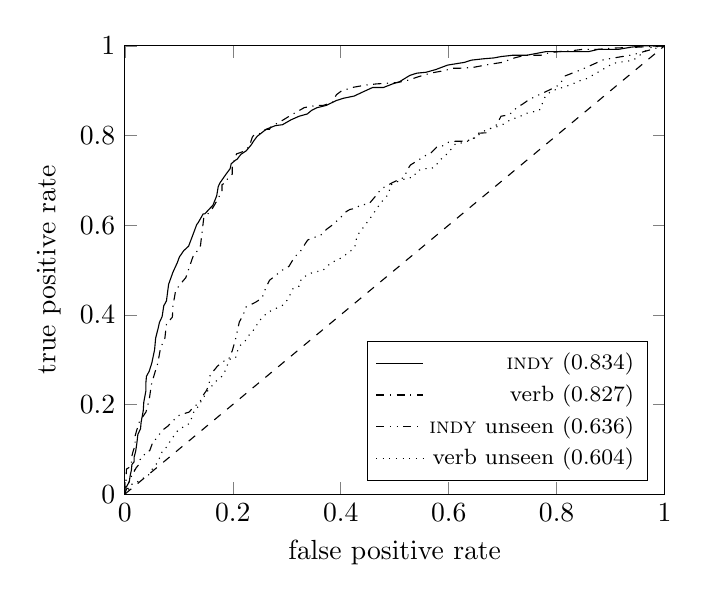
\begin{tikzpicture}
    \begin{axis}[xmin=0,xmax=1,ymin=0,ymax=1,xlabel={false positive rate},ylabel={true positive rate},legend pos=south east,legend cell align={right},legend style={font=\footnotesize}]
      \addplot [dashed,forget plot] coordinates{(0,0) (1,1)};
      \addplot [] coordinates{(0.000,0.000) (0.000,0.005) (0.000,0.016) (0.003,0.016) (0.005,0.021) (0.008,0.027) (0.010,0.043) (0.012,0.053) (0.013,0.066) (0.017,0.072) (0.017,0.082) (0.020,0.096) (0.022,0.112) (0.024,0.133) (0.029,0.146) (0.030,0.160) (0.034,0.186) (0.035,0.205) (0.037,0.218) (0.039,0.231) (0.039,0.247) (0.039,0.250) (0.040,0.263) (0.045,0.274) (0.050,0.293) (0.055,0.322) (0.057,0.348) (0.062,0.372) (0.064,0.383) (0.069,0.396) (0.072,0.420) (0.077,0.431) (0.081,0.468) (0.089,0.495) (0.097,0.516) (0.101,0.529) (0.109,0.543) (0.118,0.553) (0.124,0.572) (0.133,0.601) (0.136,0.606) (0.145,0.625) (0.148,0.625) (0.158,0.638) (0.163,0.644) (0.170,0.665) (0.173,0.686) (0.176,0.694) (0.187,0.713) (0.195,0.726) (0.197,0.737) (0.205,0.745) (0.208,0.747) (0.215,0.758) (0.225,0.766) (0.234,0.779) (0.240,0.790) (0.245,0.798) (0.262,0.814) (0.279,0.822) (0.292,0.824) (0.308,0.835) (0.323,0.843) (0.338,0.848) (0.346,0.856) (0.356,0.862) (0.373,0.867) (0.392,0.878) (0.405,0.883) (0.425,0.888) (0.439,0.896) (0.459,0.907) (0.479,0.907) (0.496,0.915) (0.509,0.920) (0.528,0.934) (0.541,0.939) (0.558,0.941) (0.576,0.947) (0.598,0.957) (0.629,0.963) (0.642,0.968) (0.664,0.971) (0.684,0.973) (0.697,0.976) (0.719,0.979) (0.745,0.979) (0.780,0.987) (0.797,0.987) (0.829,0.987) (0.859,0.987) (0.877,0.992) (0.914,0.992) (0.938,0.997) (0.961,1.000) (1.000,1.000)}; %indy auc = 0.834
      \addplot [dash dot] coordinates{(0.000,0.000) (0.000,0.005) (0.000,0.008) (0.000,0.008) (0.000,0.008) (0.000,0.011) (0.000,0.019) (0.000,0.021) (0.000,0.027) (0.002,0.029) (0.002,0.032) (0.002,0.037) (0.003,0.056) (0.010,0.061) (0.012,0.069) (0.013,0.085) (0.015,0.095) (0.019,0.109) (0.019,0.130) (0.022,0.143) (0.027,0.162) (0.039,0.183) (0.045,0.210) (0.049,0.244) (0.056,0.273) (0.061,0.292) (0.066,0.326) (0.074,0.347) (0.077,0.379) (0.088,0.395) (0.089,0.419) (0.094,0.454) (0.103,0.469) (0.113,0.483) (0.121,0.512) (0.128,0.536) (0.136,0.544) (0.140,0.554) (0.143,0.584) (0.146,0.615) (0.152,0.623) (0.158,0.631) (0.162,0.637) (0.167,0.647) (0.172,0.658) (0.180,0.676) (0.180,0.690) (0.189,0.698) (0.190,0.703) (0.199,0.714) (0.199,0.729) (0.204,0.751) (0.207,0.759) (0.219,0.764) (0.224,0.767) (0.231,0.777) (0.236,0.796) (0.239,0.801) (0.244,0.801) (0.253,0.806) (0.258,0.812) (0.264,0.814) (0.268,0.814) (0.271,0.820) (0.279,0.825) (0.291,0.833) (0.306,0.844) (0.325,0.857) (0.332,0.862) (0.354,0.867) (0.367,0.867) (0.384,0.873) (0.392,0.891) (0.401,0.899) (0.421,0.907) (0.444,0.912) (0.466,0.915) (0.505,0.918) (0.524,0.923) (0.544,0.931) (0.566,0.939) (0.589,0.944) (0.609,0.950) (0.621,0.950) (0.646,0.952) (0.672,0.958) (0.699,0.963) (0.722,0.973) (0.742,0.979) (0.771,0.979) (0.785,0.984) (0.803,0.987) (0.828,0.989) (0.848,0.992) (0.875,0.992) (0.907,0.995) (0.951,0.997) (1.000,1.000)}; %verb auc = 0.827
      \addplot [dash dot dot] coordinates {(0.000,0.000) (0.001,0.000) (0.001,0.005) (0.003,0.011) (0.004,0.013) (0.007,0.013) (0.007,0.019) (0.007,0.027) (0.011,0.039) (0.016,0.042) (0.018,0.054) (0.019,0.054) (0.021,0.059) (0.026,0.066) (0.028,0.077) (0.033,0.080) (0.038,0.093) (0.046,0.097) (0.053,0.120) (0.056,0.121) (0.065,0.135) (0.070,0.143) (0.080,0.152) (0.085,0.159) (0.099,0.175) (0.108,0.179) (0.119,0.183) (0.127,0.194) (0.139,0.205) (0.142,0.215) (0.151,0.231) (0.156,0.244) (0.158,0.267) (0.168,0.280) (0.171,0.285) (0.184,0.297) (0.192,0.300) (0.199,0.320) (0.204,0.341) (0.209,0.367) (0.212,0.384) (0.219,0.399) (0.224,0.417) (0.242,0.428) (0.254,0.437) (0.261,0.460) (0.268,0.477) (0.291,0.499) (0.304,0.508) (0.314,0.528) (0.326,0.543) (0.336,0.562) (0.339,0.567) (0.354,0.574) (0.363,0.578) (0.374,0.591) (0.383,0.599) (0.398,0.615) (0.410,0.630) (0.417,0.635) (0.429,0.638) (0.436,0.645) (0.452,0.647) (0.464,0.664) (0.475,0.681) (0.496,0.695) (0.518,0.707) (0.523,0.723) (0.529,0.734) (0.545,0.746) (0.555,0.754) (0.567,0.761) (0.578,0.774) (0.586,0.775) (0.600,0.785) (0.612,0.787) (0.623,0.787) (0.635,0.789) (0.646,0.791) (0.654,0.805) (0.670,0.806) (0.677,0.815) (0.689,0.824) (0.697,0.843) (0.712,0.846) (0.726,0.862) (0.737,0.870) (0.749,0.880) (0.759,0.886) (0.777,0.896) (0.791,0.904) (0.805,0.913) (0.816,0.933) (0.844,0.946) (0.887,0.969) (0.941,0.980) (1.000,1.000)}; %indy shuffled auc = 0.636
      \addplot [dotted] coordinates{(0.000,0.000) (0.000,0.004) (0.002,0.008) (0.006,0.009) (0.012,0.017) (0.012,0.022) (0.018,0.022) (0.026,0.030) (0.036,0.037) (0.042,0.039) (0.046,0.047) (0.052,0.058) (0.055,0.063) (0.061,0.071) (0.063,0.079) (0.067,0.084) (0.069,0.096) (0.079,0.107) (0.086,0.123) (0.091,0.130) (0.095,0.138) (0.102,0.146) (0.109,0.150) (0.120,0.158) (0.125,0.174) (0.129,0.188) (0.139,0.198) (0.142,0.211) (0.147,0.218) (0.149,0.226) (0.156,0.233) (0.166,0.249) (0.174,0.257) (0.182,0.265) (0.188,0.281) (0.192,0.296) (0.197,0.304) (0.205,0.304) (0.211,0.329) (0.222,0.340) (0.233,0.360) (0.242,0.370) (0.247,0.385) (0.258,0.396) (0.262,0.404) (0.278,0.413) (0.295,0.423) (0.303,0.437) (0.309,0.452) (0.312,0.460) (0.323,0.464) (0.327,0.481) (0.341,0.491) (0.352,0.496) (0.366,0.498) (0.382,0.516) (0.391,0.521) (0.401,0.527) (0.416,0.540) (0.426,0.551) (0.430,0.576) (0.445,0.600) (0.456,0.618) (0.465,0.634) (0.473,0.648) (0.489,0.670) (0.492,0.689) (0.499,0.694) (0.513,0.701) (0.536,0.708) (0.540,0.720) (0.552,0.726) (0.567,0.726) (0.576,0.731) (0.582,0.744) (0.589,0.750) (0.598,0.760) (0.613,0.782) (0.629,0.784) (0.642,0.791) (0.655,0.801) (0.671,0.814) (0.686,0.818) (0.701,0.825) (0.713,0.834) (0.733,0.843) (0.743,0.849) (0.757,0.853) (0.768,0.856) (0.779,0.887) (0.790,0.899) (0.816,0.909) (0.828,0.914) (0.840,0.921) (0.856,0.927) (0.875,0.940) (0.905,0.961) (0.942,0.968) (0.973,0.996) (1.000,1.000)}; %verb shuffled auc = 0.604
      \legend{\textsc{indy} (0.834),verb (0.827),\textsc{indy} unseen (0.636),verb unseen (0.604)} 
    \end{axis}
  \end{tikzpicture}
\caption[Receiver Operating Characterisation for Coercion Classification]{Receiver operating characteristic plots for a selection of models for coercion classification, with the area under the curve for each model type indicated in the legend.}
\label{fig:coerroc}
\end{figure}

Figure~\ref{fig:coerroc} presents a receiver operating characteristic plot comparing between the verb-only and \textsc{indy} techniques for both the regular and rearranged versions of the data, with areas under the curve indicated in the legend.  As expected, the verb-only and \textsc{indy} techniques are comparable for the unaltered version of the data, but the model learned from verb-only subspaces falls off once each verb stem is treated as its own fold of the data.  Of particular note is the way that the rearranged verb-only curve flattens out in the middle: the relative drop-off in true positives in the mid-range of cut-off points for classifying coercion tells us that there is a lull in the precision of the model here, with mistakes being made on the interpretation of subspaces projected by unfamiliar verbs (keeping in mind that, in the unaltered version of the data, the subspace projected by two different instances of the same verb morpheme would be identical, and so it is only the variance in the relative situation of the noun-vector in these subspaces that needs to be analysed to evaluate coercion).  The relative jumpiness of the curves as compared to the smooth trajectories observed for the metaphor data in Figure~\ref{fig:metaroc} can be attributed to the scale of the data, with the massiveness of the metaphor dataset providing a steadier progression as the criteria for positive classification are relaxed.  On the whole, though, the story here is a similar one of a fairly balanced advance of recall and a correspondingly steady decline in precision as the model becomes increasingly permissive in its classification of coercion.

\subsection{The Geometry of Coercion}
Following the procedure which has proved productive for the analysis of semantic phenomena in preceding experiments, I will now study the statistical geometry associated with the contextual classification of coercion, beginning with an analysis of individual features and moving on the a consideration of optimal combinations of features.  In Table~\ref{tab:ind-coercion}, I once again report the top five performing (in terms of f-score) features for each of the context sensitive dimension selection techniques described in the previous section.  These features have been tested on the more prohibitive version of the coercion data rearranged to avoid training and testing on the same verb stem types, and with this in mind the improvement in scores here as compared to Table~\ref{tab:verb-coercion} is remarkable.  With the exception of the \textsc{zipped} subspaces, all other techniques exhibit substantial improvements on the models learned from the full set of statistical features, with the difference in the verb-only spaces especially notable and a significant improvement at 

XXX

\begin{table}
\centering
\begin{tabular}{lr|lr|lr}
\hline
\multicolumn{2}{c}{\textsc{joint}} & \multicolumn{2}{c}{\textsc{indy}} & \multicolumn{2}{c}{\textsc{zipped}} \\
\hline
$\mu(\overline{A'X'},\overline{B'X'})$ & 0.526 & $\mu(\overline{A'X'},\overline{B'X'})$ & 0.547 & $\mu(\overline{A'C'},\overline{B'C'})$ & 0.392 \\
$\mu(\overline{A'C'},\overline{B'X'}$ & 0.496 & $\mu(\overline{A'C'},\overline{B'C'})$ & 0.544 & $\mu(A,B)/C$ & 0.349 \\
$\mu(\overline{A'M'},\overline{B'M'}$ & 0.453 & $\mu(A,B)/C$ & 0.522 & $\mu(\overline{A'X'},\overline{B'X'})$ & 0.321 \\
$\mu(A,B)/C$ & 0.442 & $\angle AOB$ & 0.517 & $\mu(\overline{A'M'},\overline{B'M'})$ & 0.237 \\
$\angle AOB$ & 0.429 & $\mu(\overline{A'M'},\overline{B'M'})$ & 0.504 & $\angle AOB$ & 0.209 \\
\hline
\end{tabular}
\vfill
\begin{tabular}{lr|lr}
\multicolumn{2}{c}{\textsc{verb}} & \multicolumn{2}{c}{\textsc{noun}} \\
\hline
$\overline{AC}/\overline{BC}$ & 0.580 & $A:B$ & 0.528 \\
$A:B$ & 0.412 & $A/B$ & 0.486 \\
$A/B$ & 0.387 & $\mu(A,B)/C$ & 0.486 \\
$\mu(\overline{A'M'},\overline{B'M'})$ & 0.384 & $\angle AMB$ & 0.427 \\
$\mu(\overline{A'X'},\overline{B'X'})$ & 0.374 & $\angle ACB$ & 0.423 \\
\hline
\end{tabular}
\caption[Top Independent Features for Coercion Classification]{Independent f-scores from the coercion classification data for top five features of each subspace type for 2x2 word co-occurrence window, 400 dimension subspaces, validated on unobserved verbs.}
\label{tab:ind-coercion}
\end{table}

Also of note is the character of the features that are most predictive for each dimensional selection technique.  For all three methods involving both words as input for subspace selection, the mean values of distances at the normalised level of subspaces feature prominently (and it should be noted that the angle $\angle AOB$, which also features here, is perfectly correlated with the distance between the normalised word-vectors $A'$ and $B'$).  This indicates that the angles formed between the word-vectors and the generic vectors are especially associated with coercion, and this as opposed to metaphor, where the distance of various vectors from the origin as well as the ratios of these distances are particular predictive.  That the averages of the angles with the generic vectors seem generally more significant than the angles between the word-vectors themselves is evidence that it is the absolute and combined situation of the word-vectors in the context of their subspaces, rather than their relationship to one another, that can be interpreted in terms of a typological semantic relationship such as coercion.

All of this is in opposition to the top features for the subspaces selected based on a single input term, where fractions and ratios are prominent.  Of particular note is the significance of the relationship between the word-vectors, and this makes sense: given that the relevance of one word-vector in a subspace selected by the other is only incidental and in no way built into the space itself, differences in the relative lengths of the word-vectors and their relative distances to generic points are particularly indicative of degrees of inclusion in the profile characteristic to the dimension-selecting term.  The implication is that, with a co-occurrence profile chosen by one word, it is simply the prominence of the other word with respect to this profile that is indicative of the typological relationship between the verb's selectional constraints and the noun's categorical expectation.  Furthermore, the resurgence of verb-only spaces here in terms of a singular feature, namely, the fraction of the verb-centre-vector distance $\overline{AC}$ to the comparable distance $\overline{BC}$ tells us that the comparative situation of the word-vectors to the absolute centre of a subspace varies between coercive and non-coercive cases of argument selection.  It's worth noting here that, in verb-selected subspaces projected from the 2x2 word window base space, co-occurrences dimensions will correspond to terms that tend to be observed in close proximity to the verbs themselves, so we can expect these dimensions to be characterised by arguments of the verbs and modifiers of those arguments: it isn't hard to imagine how, in terms of modifiers in particular, the typical characteristics of the arguments normally selected by a verb would serve as a kind of template for testing the typological fit of a new candidate argument, with relative proximity to the centre, along with the extent of the noun vector along these characteristic co-occurrence dimensions, being good metrics for determining the fit.

\begin{table}
\centering
\begin{tabular}{llr}
\hline
& \multicolumn{1}{c}{\textsc{indy} ($f = 0.681$)} & \multicolumn{1}{c}{\textsc{verb} ($f = 0.688$)} \\
\hline
& \multicolumn{2}{c}{\textsc{distances}} \\
word-vectors & - & - \\
generic vectors & - & $-0.833 = X$ \\
\hline
& \multicolumn{2}{c}{\textsc{angles}} \\
word-vectors & $\angle AMB = -0.564$ & - \\
& $\angle ACB = -0.103$ \\
normalised & - & $0.290 = \angle A'M'B'$ \\
generic & - & $1.241 = \angle COM$ \\
& & $-0.214 = \angle COX$ \\
\hline
& \multicolumn{2}{c}{\textsc{means}} \\
word-vectors & $\mu(A,B) = 1.656$ & - \\
normalised & - & $0.452 = \mu(\overline{A'X'},\overline{B'X'})$ \\
\hline
& \multicolumn{2}{c}{\textsc{ratios}} \\
word-vectors & $\overline{AM}:\overline{BM} = 0.450$ & - \\
normalised - & - \\
\hline
& \multicolumn{2}{c}{\textsc{fractions}} \\
word-vectors & - & $2.315 = \overline{AM}/\overline{BM}$ \\
normalised & $\overline{A'M'}/\overline{B'M'} = -0.259$ & - \\
& $\overline{A'X'}/\overline{B'X'} = 0.203$ & - \\
generic vectors & $C/M = -1.257$ & $-2.398 = C/M$ \\
\hline
\end{tabular}
\caption{Comparison of the seven most effective features for coercion classification in 2x2 word, 400 dimensional subspaces for \textsc{indy} versus \textsc{verb} based dimension selection.}
\label{tab:coertures}
\end{table}

These independent feature results are suggestive of the types of statistics that are associated with coercion, but not of the direction of these correlations, let alone the dynamics between different statistics.  To examine the geometry of coercion more in depth, I once again perform a beam search to discover the top seven features associated with both the \textsc{indy} and verb-only subspace selection techniques in 400 dimensional subspaces projected from 2x2 word window base spaces, training models on the rearranged version of the data and applying a vector inflation factor in order to avoid collinearity between input features.  Results are reported in Table~\ref{tab:coertures}.  Remarkably, a very different picture emerges than what was observed above regarding independent features, with neither the mean distances between the norms of the \textsc{indy} subspaces nor the angles and ratios individually observed in the verb-only subspaces making an appearance.  In fact, one of the most notable characteristics of the respective feature vectors is, on the one hand, the spread of the features across several different categories of co-occurrence statistic, but then also the balance between non-normalised features in one category for one technique versus the normalised components of the same category for the other technique.

So, for instance, the angles $\angle AMB$ and $\angle ACB$ both correlate negatively with coercion (meaning the angles are wider for more coercive word pairs) in the \textsc{indy} type subspaces, implying that the word-vectors are more likely to be found on opposite sides of these two central points in the space in the case of coercive pairings (but not necessarily on opposite sides of the lines extending from the origin through these points--they could, for instance, be above and below a point relative to the origin).  The positive correlation with the angle $\angle A'M'B'$ in the verb-only subspaces, on the other hand, indicates that the word-vectors tend to be on opposite sides of the lines extending through the mean vector.  This is interesting, since we can safely assume that the verb-vector will occupy a relatively central position in a subspace defined entirely by dimensions with which the verb has a high expectation of co-occurrence: it would seem that the noun-vector essentially pivots towards the co-occurrence dimensions that are most strongly associated with the verb, meaning that the words that are especially characteristic of the immediate syntagmatic situation of the verb tend to have a stronger association with nouns of a type not paradigmatically selected by the verb.  In the case of fractions of lengths between vectors, on the other hand, the very strong positive correlation between coercion and $\overline{AM}/\overline{BM}$ in verb-only spaces suggests that as the noun-vector (associated with $B$) retracts towards the origin relative to the verb-vector, coercion is more likely.  This makes sense in this type of subspace, since nouns of types that categorically satisfy a verb's selectional constraints will tend to have higher PMI values along the dimensions selected by that verb.  The negative value for the normalised version of the same fraction in the case of the \textsc{indy} subspaces, however, means that the respective angles between the word-vectors and the mean vector tend to be more balance in cases of coercion.

The one point of consistent comparison across the two techniques is the fraction of the length of the central vector $C$ divided by the length of the mean vector $M$.  As discussed in Chapter~\ref{sec:litpare} in the context of the comparison between relatedness and similarity, the negative correlation here for both the \textsc{indy} technique and the verb-only technique indicates an increase in the likelihood of classifying a relationship as coercive as variance across the mean values of features delineating a subspace increases.  If high variance were only associated with coercion through the \textsc{indy} technique, it could be argued that coercion simply correlates with subspaces patched together from two different independently selected co-occurrence profiles with a tendency towards have very different mean values: for instance, one word might select co-occurrence terms that occur more frequently and therefore have lower mean values than the other.  Given that this effect is even stronger for the verb-only subspaces, however, where the co-occurrence profile of just one term is in play, the prominence of this feature actually indicates that, as with similarity, there are some words (and, in particular, verbs) which just tend to be more coercive than others.  Moreover, these words tend to have a particular statistical characteristic by which the terms with which they co-occur tend to have more varied mean values.  In the end, this can be reduced to an observation that might not seem particularly surprising, even if it also wasn't immediately obvious prior to this geometric analysis: words that tend to be involved in coercive relationships also tend to co-occur with a range of other words that are more varied in terms of their own essential characteristics such as frequency.  This interpretation is further supported by the negative correlation between the length of the maximum vector $X$ and coercion in verb-only subspaces.  This generally indicates that there are some basic differences between the types of verbs, and the corresponding dimensional profiles, that tend to coerce their arguments, and specifically implies that coercive verbs tend to be observed in close proximity to at least some higher frequency words.

%verb joint shuffled f = 0.654

\begin{figure}
\footnotesize
\begin{subfigure}{0.3\textwidth} % heard noises
\centering
  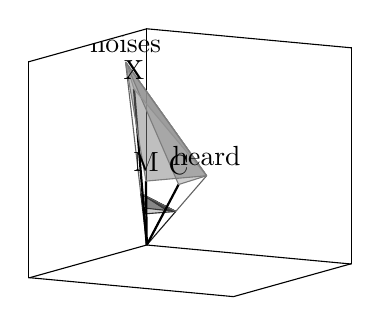
\begin{tikzpicture}
    \def\varA{(31.2371,41.3708,33.9778)};
    \def\varB{(64.4215,28.9478,79.8863)};
    \def\varC{(29.3997,29.3994,29.3996)};
    \def\varM{(36.4675,20.7482,30.9819)};
    \def\varX{(112.3873,59.9255,80.0081)};
    \def\varAN{(15.1191,20.0239,16.4456)};
    \def\varBN{(18.1248,8.1444,22.4758)};
    \def\varCN{(17.3206,17.3204,17.3205)};
    \def\varMN{(20.9761,11.9343,17.8207)};
    \def\varXN{(22.4161,11.9524,15.9580)};
    \def\nodA{31.2371,41.3708,33.9778};
    \def\nodB{64.4215,28.9478,79.8863};
    \def\nodC{29.3997,29.3994,29.3996};
    \def\nodM{36.4675,20.7482,30.9819};
    \def\nodX{112.3873,59.9255,80.0081};
    \begin{axis}[scale = 0.6,axis line style=white,view={120}{10},xmin=0,xmax=80,ymin=0,ymax=80,zmin=0,zmax=80,colormap/blackwhite,ticks=none]
      \addplot3[color=black,thick] coordinates {(0,0,80) (0,80,80)};
      \addplot3[color=black,thick] coordinates {(0,0,80) (80,0,80)};
      \addplot3[color=black,thick] coordinates {(0,80,0) (0,80,80)};
      \addplot3[color=black,thick] coordinates {(0,80,0) (80,80,0)};
      \addplot3[color=black,thick] coordinates {(80,0,0) (80,0,80)};
      \addplot3[color=black,thick] coordinates {(80,0,0) (80,80,0)};
      \addplot3[color=black] coordinates {(0,0,0) (0,0,80)};
      \addplot3[color=black] coordinates {(0,0,0) (0,80,0)};
      \addplot3[color=black] coordinates {(0,0,0) (80,0,0)};
      \addplot3[patch,patch type=triangle,color=gray,fill opacity=0.0] coordinates {(0.0,0.0,0.0) \varCN \varAN};
      \addplot3[patch,patch type=triangle,color=gray,fill opacity=0.0] coordinates {(0.0,0.0,0.0) \varCN \varBN};
      \addplot3[patch,patch type=triangle,color=darkgray,fill opacity=0.75] coordinates {\varCN \varAN \varBN};
      \addplot3[patch,patch type=triangle,color=darkgray,fill opacity=0.5] coordinates {\varMN \varAN \varBN};
      \addplot3[patch,patch type=triangle,color=darkgray,fill opacity=0.25] coordinates {\varXN \varAN \varBN};
      \addplot3 [color=black,thick] coordinates {(0,0,0) \varCN};
      \addplot3 [color=black,thick] coordinates {(0,0,0) \varXN};
      \addplot3 [color=black,thick] coordinates {(0,0,0) \varMN};
%      \addplot3[opacity = 0.1,surf,z buffer = sort,samples = 21,variable = \u,variable y = \v,domain = 0:90,y domain = 0:90,]
%    ({1*cos(u)*sin(v)}, {1*sin(u)*sin(v)}, {1*cos(v)});
      \addplot3 [patch,patch type=rectangle,color=lightgray,fill opacity=0.0] coordinates{\varAN \varA \varB \varBN
};
      \addplot3 [color=black,thick] coordinates {\varCN \varC};
      \addplot3 [color=black,thick] coordinates {\varXN \varX};
      \addplot3 [color=black,thick] coordinates {\varMN \varM};
      \addplot3 [patch,patch type=triangle,color=lightgray,fill opacity=0.75] coordinates{\varA \varC \varB};
      \addplot3 [patch,patch type=triangle,color=gray,fill opacity=0.25] coordinates{\varA \varX \varB};
      \addplot3 [patch,patch type=triangle,color=gray,fill opacity=0.5] coordinates{\varA \varM \varB};
      \node [anchor=south] at (axis cs: \nodA) {heard};
      \node [anchor=south] at (axis cs: \nodB) {noises};
      \node [anchor=south] at (axis cs: \nodC) {C};
      \node [anchor=south] at (axis cs: \nodX) {X};
      \node [anchor=south] at (axis cs: \nodM) {M};
    \end{axis}
  \end{tikzpicture}
\caption*{\footnotesize \emph{non-coercive: heard noises}}
\end{subfigure}
\hfill
\begin{subfigure}{0.3\textwidth} % hear click
\centering
  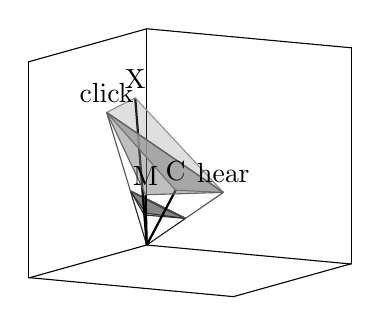
\begin{tikzpicture}
    \def\varA{(26.6923,45.2717,27.4741)};
    \def\varB{(45.5472,10.6624,56.8395)};
    \def\varC{(26.6298,26.6294,26.6297)};
    \def\varM{(34.7432,19.5859,25.5589)};
    \def\varX{(110.7493,59.4545,76.4383)};
    \def\varAN{(13.5030,22.9019,13.8985)};
    \def\varBN{(18.5620,4.3453,23.1640)};
    \def\varCN{(17.3206,17.3204,17.3205)};
    \def\varMN{(22.0031,12.4039,16.1866)};
    \def\varXN{(22.5841,12.1240,15.5874)};
    \def\nodA{26.6923,45.2717,27.4741};
    \def\nodB{45.5472,10.6624,56.8395};
    \def\nodC{26.6298,26.6294,26.6297};
    \def\nodM{34.7432,19.5859,25.5589};
    \def\nodX{110.7493,59.4545,76.4383};
    \begin{axis}[scale = 0.6,axis line style=white,view={120}{10},xmin=0,xmax=80,ymin=0,ymax=80,zmin=0,zmax=80,colormap/blackwhite,ticks=none]
      \addplot3[color=black,thick] coordinates {(0,0,80) (0,80,80)};
      \addplot3[color=black,thick] coordinates {(0,0,80) (80,0,80)};
      \addplot3[color=black,thick] coordinates {(0,80,0) (0,80,80)};
      \addplot3[color=black,thick] coordinates {(0,80,0) (80,80,0)};
      \addplot3[color=black,thick] coordinates {(80,0,0) (80,0,80)};
      \addplot3[color=black,thick] coordinates {(80,0,0) (80,80,0)};
      \addplot3[color=black] coordinates {(0,0,0) (0,0,80)};
      \addplot3[color=black] coordinates {(0,0,0) (0,80,0)};
      \addplot3[color=black] coordinates {(0,0,0) (80,0,0)};
      \addplot3[patch,patch type=triangle,color=gray,fill opacity=0.0] coordinates {(0.0,0.0,0.0) \varCN \varAN};
      \addplot3[patch,patch type=triangle,color=gray,fill opacity=0.0] coordinates {(0.0,0.0,0.0) \varCN \varBN};
      \addplot3[patch,patch type=triangle,color=darkgray,fill opacity=0.75] coordinates {\varCN \varAN \varBN};
      \addplot3[patch,patch type=triangle,color=darkgray,fill opacity=0.5] coordinates {\varMN \varAN \varBN};
      \addplot3[patch,patch type=triangle,color=darkgray,fill opacity=0.25] coordinates {\varXN \varAN \varBN};
      \addplot3 [color=black,thick] coordinates {(0,0,0) \varCN};
      \addplot3 [color=black,thick] coordinates {(0,0,0) \varXN};
      \addplot3 [color=black,thick] coordinates {(0,0,0) \varMN};
%      \addplot3[opacity = 0.1,surf,z buffer = sort,samples = 21,variable = \u,variable y = \v,domain = 0:90,y domain = 0:90,]
%    ({1*cos(u)*sin(v)}, {1*sin(u)*sin(v)}, {1*cos(v)});
      \addplot3 [patch,patch type=rectangle,color=lightgray,fill opacity=0.0] coordinates{\varAN \varA \varB \varBN
};
      \addplot3 [color=black,thick] coordinates {\varCN \varC};
      \addplot3 [color=black,thick] coordinates {\varXN \varX};
      \addplot3 [color=black,thick] coordinates {\varMN \varM};
      \addplot3 [patch,patch type=triangle,color=lightgray,fill opacity=0.75] coordinates{\varA \varC \varB};
      \addplot3 [patch,patch type=triangle,color=gray,fill opacity=0.25] coordinates{\varA \varX \varB};
      \addplot3 [patch,patch type=triangle,color=gray,fill opacity=0.5] coordinates{\varA \varM \varB};
      \node [anchor=south] at (axis cs: \nodA) {hear};
      \node [anchor=south] at (axis cs: \nodB) {click};
      \node [anchor=south] at (axis cs: \nodC) {C};
      \node [anchor=south] at (axis cs: \nodX) {X};
      \node [anchor=south] at (axis cs: \nodM) {M};
    \end{axis}
  \end{tikzpicture}
\caption*{\footnotesize \emph{neutral: hear click}}
\end{subfigure}
\hfill
\begin{subfigure}{0.3\textwidth} % hear motor
\centering
  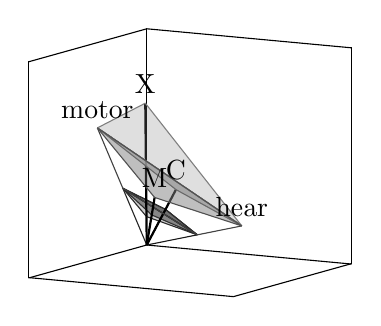
\begin{tikzpicture}
    \def\varA{(22.0152,49.7517,14.7908)};
    \def\varB{(37.5202,2.4240,49.1531)};
    \def\varC{(26.9425,26.9422,26.9425)};
    \def\varM{(33.6557,22.5056,24.6651)};
    \def\varX{(112.2882,64.2694,75.1433)};
    \def\varAN{(11.7145,26.4732,7.8703)};
    \def\varBN{(18.1889,1.1751,23.8282)};
    \def\varCN{(17.3206,17.3204,17.3206)};
    \def\varMN{(21.2972,14.2415,15.6080)};
    \def\varXN{(22.5149,12.8867,15.0670)};
    \def\nodA{22.0152,49.7517,14.7908};
    \def\nodB{37.5202,2.4240,49.1531};
    \def\nodC{26.9425,26.9422,26.9425};
    \def\nodM{33.6557,22.5056,24.6651};
    \def\nodX{112.2882,64.2694,75.1433};
    \begin{axis}[scale = 0.6,axis line style=white,view={120}{10},xmin=0,xmax=80,ymin=0,ymax=80,zmin=0,zmax=80,colormap/blackwhite,ticks=none]
      \addplot3[color=black,thick] coordinates {(0,0,80) (0,80,80)};
      \addplot3[color=black,thick] coordinates {(0,0,80) (80,0,80)};
      \addplot3[color=black,thick] coordinates {(0,80,0) (0,80,80)};
      \addplot3[color=black,thick] coordinates {(0,80,0) (80,80,0)};
      \addplot3[color=black,thick] coordinates {(80,0,0) (80,0,80)};
      \addplot3[color=black,thick] coordinates {(80,0,0) (80,80,0)};
      \addplot3[color=black] coordinates {(0,0,0) (0,0,80)};
      \addplot3[color=black] coordinates {(0,0,0) (0,80,0)};
      \addplot3[color=black] coordinates {(0,0,0) (80,0,0)};
      \addplot3[patch,patch type=triangle,color=gray,fill opacity=0.0] coordinates {(0.0,0.0,0.0) \varCN \varAN};
      \addplot3[patch,patch type=triangle,color=gray,fill opacity=0.0] coordinates {(0.0,0.0,0.0) \varCN \varBN};
      \addplot3[patch,patch type=triangle,color=darkgray,fill opacity=0.75] coordinates {\varCN \varAN \varBN};
      \addplot3[patch,patch type=triangle,color=darkgray,fill opacity=0.5] coordinates {\varMN \varAN \varBN};
      \addplot3[patch,patch type=triangle,color=darkgray,fill opacity=0.25] coordinates {\varXN \varAN \varBN};
      \addplot3 [color=black,thick] coordinates {(0,0,0) \varCN};
      \addplot3 [color=black,thick] coordinates {(0,0,0) \varXN};
      \addplot3 [color=black,thick] coordinates {(0,0,0) \varMN};
%      \addplot3[opacity = 0.1,surf,z buffer = sort,samples = 21,variable = \u,variable y = \v,domain = 0:90,y domain = 0:90,]
%    ({1*cos(u)*sin(v)}, {1*sin(u)*sin(v)}, {1*cos(v)});
      \addplot3 [patch,patch type=rectangle,color=lightgray,fill opacity=0.0] coordinates{\varAN \varA \varB \varBN
};
      \addplot3 [color=black,thick] coordinates {\varCN \varC};
      \addplot3 [color=black,thick] coordinates {\varXN \varX};
      \addplot3 [color=black,thick] coordinates {\varMN \varM};
      \addplot3 [patch,patch type=triangle,color=lightgray,fill opacity=0.75] coordinates{\varA \varC \varB};
      \addplot3 [patch,patch type=triangle,color=gray,fill opacity=0.25] coordinates{\varA \varX \varB};
      \addplot3 [patch,patch type=triangle,color=gray,fill opacity=0.5] coordinates{\varA \varM \varB};
      \node [anchor=south] at (axis cs: \nodA) {hear};
      \node [anchor=south] at (axis cs: \nodB) {motor};
      \node [anchor=south] at (axis cs: \nodC) {C};
      \node [anchor=south] at (axis cs: \nodX) {X};
      \node [anchor=south] at (axis cs: \nodM) {M};
    \end{axis}
  \end{tikzpicture}
\caption*{\footnotesize \emph{coercive: hear motor}}
\end{subfigure}
\caption[Coercion in Space]{Three dimensional projections of word-vectors and generic vectors in \textsc{indy} subspaces for pairs at the extents and in the middle of the spectrum of coercion.}
\label{fig:coerspaces}
\end{figure}

Figure~\ref{fig:coerspaces} illustrates word-vectors and generic vectors projected into exemplary instances of subspaces at three different phases of coercion.  Similarly to the literal stage of metaphor illustrated in Figure~\ref{fig:metaspaces}, the least coercive instance is characterised by a relatively tight space, with the noun-vector particularly prominent and acute angles at the vertexes of the generic points.  The next two stages of coercion go through something of the reverse of the process observed with metaphor, however, beginning with a contraction and a bit of an widening in the somewhat neutral case of \emph{hear click}, and then opening up into a more disparate arrangement across the subspace for the unambiguously coercive \emph{hear motor}.  The angles at the vertices of the generic point in particular, as well as the balance between the distances between the word-vectors and these points, follow the trend indicated by the coefficient weightings reported for \textsc{indy} subspaces in Table~\ref{tab:coertures}.  The shift in the overall balance of the word-vectors is interesting to note, as well: while the ratio $A:B$ wasn't indicated in the feature-wise analysis of the space, the prominence of the vector for \emph{noise} in the projection on the left suggests that there could be some nouns which are less likely to be susceptible to coercion, and indeed it is tricky to imagine the context in which the fairly abstract word \emph{noise} could be adapted to a conceptual category other than \textsc{noise}.

A more general implication of this geometric analysis is the idea that coercion is a graduated rather than a binary phenomenon.  This runs counter to what has been the conventional approach to this semantic phenomenon in the field, which considers coercion to be effectively an activation of a rule based process of constraint satisfaction: \cite{Pustejovsky} surveys the typical approach to coercion, and indeed to lexical ambiguity in general, as a process of contextualised \emph{selectional restriction} over a set of discreet word senses \citep[though see][for computational applications of a probabilistic, corpus based model]{LapataEA2003,ShutovaEA2013b}.  It seems apparent, though, that some instances of predicate type coercion are less obvious than others.  \emph{Hear click} illustrates this point nicely, as we are are forced to pause while we consider whether \emph{click} categorically denotes \textsc{noise} or something more like \emph{process} or even \emph{event}.  Furthermore, to borrow an instance from \emph{BriscoeEA1995}, among others, phrases such as \emph{enjoy a book} are clearly coercive and moreover open to interpretation as to the exact mechanism of type shifting: is the book being read or written?

The prodigious use of terms such as \emph{book} in the literature suggests that the axis of concretion and abstraction may be involved in these determinations.  To the extent that concrete terms might be understood as relatively low level nodes in a conceptual taxonomy working its way up to the more abstract types, the distance of a word like \emph{motor} from a paradigmatic denotation such as \textsc{entity} could therefore facilitate its coercion into the class \textsc{noise}.  Rather than modelling this semantic phenomenon as a consequence of a symbolic system of typed representations, however, I have sought to explore the extent to which co-occurrence features can prefigure subsequent high-level decisions about coercion.  To the degree that the output of my methodology can be considered a positive result, the finding might be summarised like this: there is evidence here for a lexical semantic model grounded in statistical, interactive, contextually adjustable representations, with categorical commitments regarding the conceptual indices of semantic units emerging from the dynamics of the representation in the course of language use.

\subsection{Adding Sentential Context}
To revisit \citepos{Pustejovsky2008} hypothesis regarding the mechanisms of semantic type coercion, the explication of type shifts arises fundamentally in a conceptual and, accordingly, linguistic context.  While I have, as discussed in Chapter~\ref{sec:sensitivity}, endeavoured to treat context as a more generally cognitive rather than strictly textual phenomenon, one of the appealing things about the data provided by \cite{PustejovskyEA2010} is that the word pairs classified in terms of coercion are embedded in sentences, and these sentences do naturally offer the basis for some sort of conceptual handle on the interaction between predicate and object.  In this section, I will perform a final experiment on semantic type coercion in which the content of each sentence is provided to my models as an additional input for projecting co-occurrence subspaces in which the relationship between word-vectors and generic vectors can be analysed.

To begin with, I take each sentence and, using the Stanford Parser \cite{ToutanovaEA2000},\footnote{As provided by the \texttt{nltk} package for python.} extract a part-of-speech tag for each word in each sentence in the data.  (Note that, now that I'm using the full sentences which provide unique data for every word-pair, I can use full data set of 1,992 sentences.)  For each sentence, I group together all the words other than the target verb and object that satisfy one of four grammatical class descriptions: nouns, verbs, adjectives, and adverbs.  I then run four different experiments, one treating the words for each of these grammatical classes as the input for dimension selection and then analyse the situation of the word-vectors in the projected subspaces in terms of the now familiar catalogue of geometric statistical features.  I treat the output for each grammatical class as the data for a logistic regression, first applying standard mean normalisation and then, setting values for sentences where no words of a particular grammatical class are available to zero, train a model to learn to classify each word pair as coercive or not coercive.  Results for each grammatical class, with various dimensional and co-occurrence window parameters, using the \textsc{joint} and \textsc{indy} dimension selection techniques, are reported in Table~\ref{tab:poses}.

\begin{table}
\centering
\begin{tabular}{llrrrr|rrrr}
\hline
\multicolumn{2}{l}{\emph{window}} & \multicolumn{4}{c}{2x2} & \multicolumn{4}{c}{5x5} \\
\multicolumn{2}{l}{\emph{dimensions}} & 20 & 50 & 200 & \multicolumn{1}{c}{400} & 20 & 50 & 200 & 400 \\
\hline
\parbox[t]{2mm}{\multirow{4}{*}{\rotatebox[origin=c]{90}{\textsc{joint}}}} & nouns & 0.157 & 0.174 & 0.244 & 0.283 & 0.193 & 0.244 & 0.257 & 0.271 \\
& verbs & 0.121 & 0.155 & 0.190 & 0.237 & 0.117 & 0.163 & 0.215 & 0.229 \\
& adjectives & 0.083 & 0.113 & 0.179 & 0.187 & 0.119 & 0.131 & 0.183 & 0.207 \\
& adverbs & 0.042 & 0.091 & 0.155 & 0.154 & 0.101 & 0.128 & 0.171 & 0.174 \\
\hline
\parbox[t]{2mm}{\multirow{4}{*}{\rotatebox[origin=c]{90}{\textsc{indy}}}} & nouns & 0.092 & 0.133 & 0.147 & 0.157 & 0.158 & 0.170 & 0.148 & 0.168 \\
& verbs & 0.117 & 0.126 & 0.173 & 0.165 & 0.147 & 0.209 & 0.174 & 0.201 \\
& adjectives & 0.123 & 0.114 & 0.162 & 0.172 & 0.173 & 0.161 & 0.151 & 0.184 \\
& adverbs & 0.115 & 0.137 & 0.139 & 0.120 & 0.167 & 0.146 & 0.121 & 0.111 \\
\hline
\end{tabular}
\caption[Correlations for Part-of-Speech Based Subspaces]{F-scores for coercion detection in full featured subspaces based on \textsc{joint} and \textsc{indy} analyses of parts of speech found in each sentence containing a verb-noun pair.}
\label{tab:poses}
\end{table}

The scores here are, clearly, low, with the top score of $f = 0.283$ for nouns in the 2x2 word window, 400 dimensional \textsc{joint} subspaces not significantly better than the minority class baseline of $f = 0.229$

XXX SIGNIFICANCE

Beyond that, it is notable that the 

We might reasonably speculate that building word-vectors based on dependency relationships -- for instance, treating the distance between words in a parse tree rather than absolute distance in a string as the boundary condition for co-occurrence window size, as \cite{WHO} have proposed -- might significantly enhance a model's ability to classify coercion.  But this would come at the expense of building a model that doesn't have some degree of syntactic commitment already built into it, and it is likewise easy to imagine how such an approach would open itself up to accusations of tautology: if coercion as a binary case is a grammatical abstraction, then such a model would be to some extent recapitulating the 

\begin{table}
\centering
\begin{tabular}{lrrrr|rrrr}
\hline
\emph{window} & \multicolumn{4}{c}{2x2} & \multicolumn{4}{c}{5x5} \\
\emph{dimensions} & 20 & 50 & 200 & \multicolumn{1}{c}{400} & 20 & 50 & 200 & 400 \\
\hline
\textsc{joint} & 0.348 & 0.369 & 0.352 & 0.371 & 0.369 & 0.392 & 0.362 & 0.383 \\
\textsc{indy} & 0.411 & 0.406 & 0.467 & 0.494 & 0.402 & 0.358 & 0.421 & 0.438 \\
\hline
\end{tabular}
\caption[F-Scores for Coercion Classification Using Full Sentences]{F-scores for coercion identification using sentential context to generate additional subspaces and corresponding feature vectors.}
\label{tab:full-coercion}
\end{table}

\section{Interpretation and Composition in Context}
One of the tricky things about figurative language is its ephemerality: if we stare at it for long enough through a theoretical lens, it seems to vanish, as is evident in the deflationary case made by \cite{WilsonEA}.  But on the other hand, if we ask someone in street whether the phase \emph{buy a story} is more metaphoric than \emph{buy a book}, we can reasonably expect the answer will almost always be ``yes'', and it would be a mistake to dismiss the evidence that in a colloquial sense some compositions are clearly metaphoric, and others are clearly not.  This raises a challenging point with regard to the comparison between metaphor and coercion, the two instances of figurative language explored in this chapter: is metaphor perhaps to some extent a more overt case of coercion, or maybe a specific case that is in some way or another a little more subtle?  Part of the problem here is that the distinctions between these phenomena begin to exceed the capacity for what can reliably be quantified about language in a clinical setting, with evaluative criteria that will depend on the opinion of an expert which comes pre-packaged with inevitable biases.

The experiments presented in this chapter have focused on the classification of non-literal language: the simple task of determining whether the way that a set of words are used pertains to some encyclopaedic sense of their lexical semantic role, without regard to the explication of any sort of interpretation of how semantics are subverted or what the metaphor communicates.  But \cite{Shutova2010} has made the case that, in a cognitively plausible sense, metaphor classification should be seen precisely as metaphor interpretation, and this theoretical stance has been backed up by a data-driven computational model that involves classification of metaphor by way of a round-trip paraphrasing technique.  This in turn invites a consideration of the entanglement between the interpretation and composition of figurative language: metaphor and metonymy are things that, in some particular conceptual context, are done by one lexical entity to another, as the apt term \emph{coercion} would itself suggest.  If composition happens in some cognitive context, then interpretation presumably involves the identification or simulation of that context, as the relevance theoretical account of metaphor survey in Chapter~\ref{sec:words} \cite{SperberEA2012}.  This is likewise in line with \citepos{Carston2010} description of how metaphor involves the generation of an \emph{ad hoc} concept pertaining to the semantics of the shifted lexeme in the specific context of a particular linguistic encounter.

In fact, it is tempting to go so far as to say that figurative language is identified precisely as those instances of language where recourse to a conceptual context is necessary to interpret a lexical composition, and furthermore that the degree of figurativeness correlates with the extent of context construction involved in an interpretation.  If this postulate holds water, it means that metaphoricity is as much about perception 

If this postulate is accepted, then my context sensitive methodology would seem to offer a good framework for identifying metaphor, because the models produced by the methodology are indicative of the extent to which contextualisation is required in any given instance to get from a generic semantic representation to a 


This hypothesis is supported by the evidence from the metaphor experiments in Section~\ref{sec:metsperiment}, where strong results for both metaphor classification and the translation of metaphor classification models to the task of rating metaphoricity on a continuous scale indicate that the relationship between lexical semantic concepts in context sensitive spaces does tell us something about the degree to which ad hoc concepts are being extrapolated in the course of composing the input terms.  The lower numbers associated with the coercion results described in Section~\ref{sec:coersperiment} are to some extent a natural product of the nature of the data, given that 



This, then, raises a valid question: is the role of figurative language exclusively, or even for that matter primarily, to port attributes from one conceptual domain to another?  Or is what metaphor does, as \cite{Davidson1978} has famously suggested, really about something more fundamentally phenomenological than just the efficient transmission of propositions?  So, where, for instance, \cite{Sweetser1990} sees polysemy as an intermediate stage bridging the progress from literal to metaphoric usage, my methodology leaves itself open to the possibility that all usage is, in fact, first and foremost pragmatic, and only secondarily lexicalised.  By this interpretation, words have semantic affordances in terms of their potential to convey cognitive content intersubjectively, and they are picked up and used in much the same way that a cognitive agent might adapt an object designed or just perceived as being for one purpose as an implement in another activity---using a shoe as a hammer, for example, or a chair to fend off a lion.  The cognitive foregrounding of this nascent theory can be found in the ecological psychology of \cite{Gibson1979} and \cite{Bateson1972}, and the linguistic correlary seems to be in line with what psycholinguists inspired by biosemiotics such as \cite{RaczasekLeonardiEA2015} are saying about the way that language is primarily about affording cognitive value to interlocutors, including but hardly limited to truth values.

This theoretical speculation is a potential extrapolation of my methodology rather than a precondition for it, and is offered primarily as an example of how this statistical approach might become a component of productive line of philosophical enquiry.  The point, though, is that with a geometric methodology, relationships between lexical semantic representations can be recast as Gibsonian affordances: there is a mechanism for the direct perception of opportunities for meaning making in the actual layout of the statistical environment.  Meaning is, then, something which is directly perceived and acted upon, in the sense that a geometric mode of representation allows us, in an abstract sense, to imagine how an agent might participate in symbolically grounded semantic activity without resorting to the computation of the conceptual transpositions involved in the analysis of figurative language.  By situating semantic representations in a space in which the 

where metaphor is first and foremost identifiable inasmuch as there is a call to contxtualisation, measurable in terms of the various probabilistic contingencies of the space in which 

  It would be a mistake to go any further than this in terms of arguing for the cognitive plausibility of a model that is fundamentally statistical and computational, but, inasmuch as it it a desirable thing to consider the possibility that the prolific use of metaphor in the course of ordinary linguistic communication 

%\chapter{Evaluation}
This section for now very broadly outlines some of the evaluative objectives of this project.

but the crucial

considered here is the necessity of resorting to some real world mechanisms for assessing the model's performance, both through formal studies with human subjects and through a less structured but more public testing of the system 

\section{Taxonomy and Analogy}
One problem inherent in the use of datasets, be they test sets specifically designed to examine features of computational language models or general and highly public frameworks such as WordNet or DBpedia, is the necessarily biased and incomplete process of assigning conceptual relationships to senses of words.  As such, in addition to the straightforward analysis of results over test sets and reporting of precision, recall, and related statistics for ontology recapitulation, it will probably be necessary to resort to asking human subjects about the efficacy of the model's conceptual mappings.

\section{Metaphor}
Even more than with the only moderately controversial tasks of determining whether conceptual and analogical relationships are appropriately captured by the models output, the problem of assessing the creative value of metaphoric artefacts generated by the model is fraught with the 

In the end, the criteria of usefulness and novelty generally taken as the basic standard for computationally creative output can serve as a good guide for the model's target, but not as much more than this.  Simply asking humans whether they consider the model to be performing along these lines must be a hopelessly subjective enterprise

%\chapter{Conclusion}


\bibliographystyle{apalike}
\bibliography{Mega.bib}

% Start the appendix (inc. author's publications)
\begin{appendix}
%\chapter{Author's publications}

% publications goes here

\subsection*{Journal papers}
\begin{enumerate}
  \item \textbf{Y. Gao}, X. Chen, Z. Ying and C. G. Parini, ``Design and Performance
Investigation of a Dual-element PIFA Array at 2.5 GHz for MIMO Terminals," \emph{IEEE Trans. on
Antennas and Propagation}. (Revising)

\end{enumerate}


\subsection*{Conference papers}


\begin{enumerate}
  \item \textbf{Y. Gao}, X. Chen, Z. Ying and C. G. Parini , ``Further Investigation of a
Dual-Element Diversity PIFA for MIMO Applications at 2.5 GHz Band," \emph{IEEE International
Symposium on Antennas and Propagation (AP-S)} , Honolulu, Hawaii, USA  June, 2007. (Accepted)
    
\end{enumerate}

\subsection*{Project report}
\begin{enumerate}
  \item X. Chen and \textbf{Y. Gao}, ``Final Report on Modelling of Difficult Environments,"
  Galileo Advance Concept project final report (GAC/EUT/DT/219), 9th June - 31 October 2007.
  
\end{enumerate}



\renewcommand{\thefigure}{B.\arabic{figure}}
\chapter{Solutions for the Examples in Chapter 2}
\label{examples_solutions}
\section{Example 1: Antenna Spacing Effect}

\textbf{Step 1:} Get the $H_{norm}H_{norm}^\dagger$, set $2{\pi}R/\lambda={\omega}_1$ and
$2{\pi}(\overline{R})/\lambda={\omega}_2$ ($\lambda$ is the wavelength), so
\begin{equation}
H_{norm} = \frac{1}{\sqrt 2 }\left( {{\begin{array}{*{20}c}
 {e^{ - j\omega _1 }} \hfill & {e^{ - j\omega _2 }} \hfill \\
 {e^{ - j\omega _2 }} \hfill & {e^{ - j\omega _1 }} \hfill \\
\end{array} }} \right)
\end{equation}
Note: $H_{norm}^\dagger=(\overline{H_{norm}})^T$ and $e^{j\theta}=cos\theta +jsin\theta$
\begin{equation}
\begin{array}{l}
 H_{norm}H_{norm}^\dagger = \frac{1}{2}\left( {{\begin{array}{*{20}c}
 {e^{ - j\omega _1 }} \hfill & {e^{ - j\omega _2 }} \hfill \\
 {e^{ - j\omega _2 }} \hfill & {e^{ - j\omega _1 }} \hfill \\
\end{array} }} \right)\left( {{\begin{array}{*{20}c}
 {e^{j\omega _1 }} \hfill & {e^{j\omega _2 }} \hfill \\
 {e^{j\omega _2 }} \hfill & {e^{j\omega _1 }} \hfill \\
\end{array} }} \right) \\
 = \frac{1}{2}\left( {{\begin{array}{*{20}c}
 {1 + 1} \hfill & {e^{ - j(\omega _1 - \omega _2 )} + e^{ - j(\omega _1 -
\omega _2 )}} \hfill \\
 {e^{ - j(\omega _1 - \omega _2 )} + e^{ - j(\omega _1 - \omega _2 )}}
\hfill & {1 + 1} \hfill \\
\end{array} }} \right) \\
 = \left( {{\begin{array}{*{20}c}
 1 \hfill & {\cos (\omega _1 - \omega _2 )} \hfill \\
 {\cos (\omega _1 - \omega _2 )} \hfill & 1 \hfill \\
\end{array} }} \right) \\
 \end{array}
\end{equation}
\textbf{Step 2:} Get the eigenvalue of $H_{norm}H_{norm}^\dagger$, here set $\lambda$ as
eigenvalue, then,
\begin{equation}
\left( {{\begin{array}{*{20}c}
 {1 - \lambda } \hfill & {\cos (\omega _1 - \omega _2 )} \hfill \\
 {\cos (\omega _1 - \omega _2 )} \hfill & {1 - \lambda } \hfill \\
\end{array} }} \right) = 0
\end{equation}
and $\omega_1-\omega_2=2{\pi}R/\lambda-2{\pi}(\overline{R})/\lambda=-54^o$, so
$\lambda=1{\pm}cos(\omega_1-\omega_2){\approx}1{\pm}0.59$. Hence, $\lambda_1=1.59$ and
$\lambda_2=0.41$.





\end{appendix}

\end{document}
% That's all of it!
